% TIPOLOGIA DI DOCUMENTO
\documentclass{report}

% PACCHETTI INSERITI 
\usepackage{graphicx} % Per le immagini
\usepackage{amsmath} % Simboli matematici
\usepackage[hidelinks]{hyperref} % Collegamenti ipertestuali
\usepackage{amssymb} % Simboli matematici 2
\usepackage{array}
\usepackage[table]{xcolor}
\usepackage{tikz}
\usepackage{multicol}
\usepackage{fancyvrb}
\usepackage{cancel}

\usepackage{geometry}
\geometry{
 a4paper,
 total={160mm,260mm},
 left=30mm,
 top=18mm,
}
% RIDENOMINAZIONI
\renewcommand{\chaptername}{Capitolo}
\renewcommand{\contentsname}{Indice}
\renewcommand{\figurename}{Immagine}
\renewcommand{\tablename}{Tabella}
% TITOLO, INDICE
\title{\textbf{\Huge Reti di Calcolatori}\\ {\Large \textbf{\textit{Appunti del corso}}}}
\author{ \textit{Damiano Trovato}}
\date{Secondo semestre, anno 2024/25}

\begin{document}
\maketitle
\newpage
\tableofcontents
\newpage

% APPUNTI VERI E PROPRI

\chapter{Introduzione alle reti di calcolatori}

\section{L'importanza delle interconnessioni}
Tutto il mondo è connesso tramite le reti: Internet è la più grande rete di interconnessione esistente,\\ e il suo utilizzo ha stravolto il mondo per com'era conosciuto. 
Le reti velocizzano il trasferimento di dati: ciò avviene tramite un canale fisico, che permette il trasferimento di informazioni secondo dei protocolli stabiliti. Partecipano a queste interconnessioni non solo calcolatori, ma dispositivi (\textit{devices}) di qualsiasi tipo: server, data-center, dispositivi IoT e altro ancora. Data l'importanza delle reti al giorno d'oggi, diventa altrettanto importante \textbf{creare un'infrastruttura solida}, e un \textbf{insieme di protocolli} che assicurino la stabilità del sistema.

\subsection{Cos'è una rete informatica}
È un'infrastruttura che permette di collegare più dispositivi (\textit{devices}), e metterli in comunicazione.\\
Individuiamo due tipi di interconnessioni:
\begin{itemize}
    \item \textbf{Connessione fisica.}\\
    Si riferisce al mezzo fisico (cavo, sistemi wireless).
    \item \textbf{Struttura logica.}\\
    Si riferisce ai protocolli che garantiscono il funzionamento della rete.
\end{itemize}

\newpage

\section{Cos'è un protocollo}\label{1.2.1}
I \textbf{protocolli di rete} sono delle \textbf{regole} che definiscono il \textbf{formato}, e l'\textbf{ordine}, la \textbf{semantica} e la \textbf{sintassi} dei \textbf{messaggi} mandati e ricevuti tra entità interconnesse tramite la rete, nonché le azioni da effettuare per \textbf{garantire un determinato servizio}. Garantire che i \textbf{protocolli} vengano usati dai \textbf{devices} appartenenti a una \textbf{rete} è condizione necessaria per permetterne la \textbf{mutua comunicazione}.

\subsection{Stack di protocolli}
I protocolli di rete differiscono tra loro non solo per le loro caratteristiche, ma anche per il \textbf{livello} di appartenenza negli stack dei protocolli (ISO/OSI, TCP/IP).\\
Ogni protocollo è infatti associato (più o meno rigidamente) ad un livello di uno stack, un'astrazione che ordina insiemi di protocolli dall'alto verso il basso, dipendentemente dal loro ruolo. In \textbf{alto} abbiamo i protocolli più astratti e vicini all'\textbf{utente}, in \textbf{basso} quelli più vicini al \textbf{sistema fisico}. Un messaggio che sfrutta un protocollo del livello più alto, "passa"\footnote{Un esempio? Una richiesta HTTP (protocollo del layer applicativo) sfrutta il protocollo TCP (del layer di trasporto), che sfrutta IP (del layer di rete). Un protocollo del livello $n$-esimo sfrutterà protocolli di tutti i livelli inferiori} attraverso protocolli dei layer inferiori.
Ogni layer aggiunge un \textbf{header} al \textit{payload}, fornendo informazioni specifiche, per permettere la consegna del messaggio e la sua corretta interpretazione.
Il ricevente, infatti, sfrutterà gli header relativi ai vari protocolli (dal basso verso l'alto) per \textbf{interpretare} l'informazione. 

\begin{figure}[htp]
    \centering
    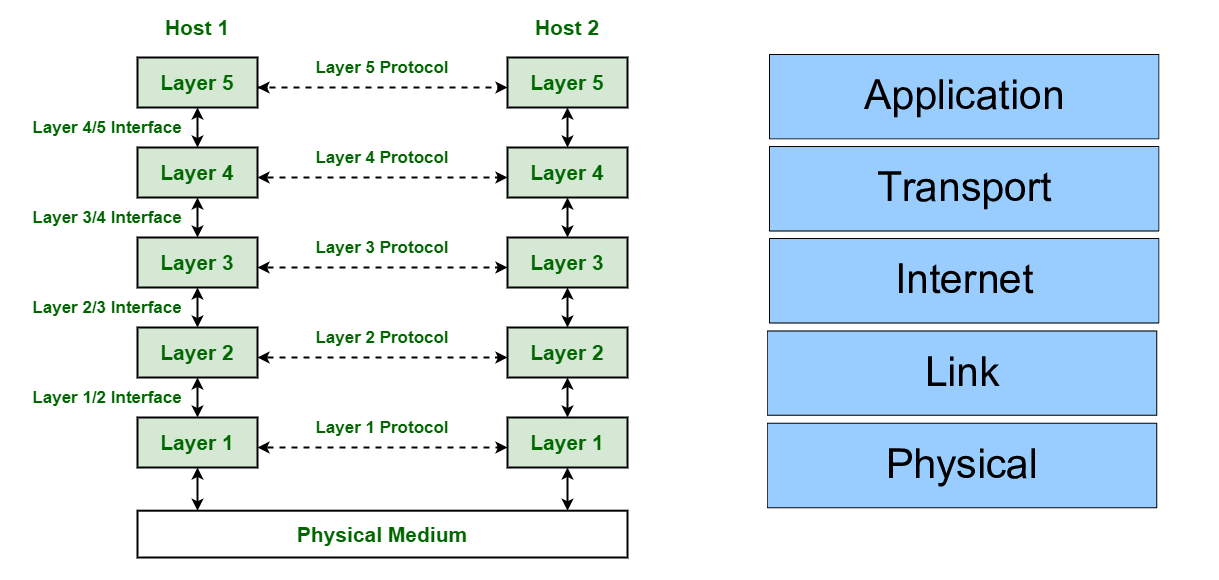
\includegraphics[width=0.9\linewidth]{./images/introduzione.png}
    \caption{Lo stack di nostro riferimento.}
\end{figure}

\subsection{Header}
Un \textbf{header} è un insieme di dati, sotto forma di bitstream, che offrono dati relativi al protocollo di appartenenza. Ogni protocollo, di un dato livello, inserirà un header con dei dati fondamentali per la trasmissione e l'interpretazione del messaggio. 

\subsection{Il mezzo fisico}
È fondamentale che il canale fisico sia gestito in maniera opportuna: il segnale che viene mandato è soggetto alla \textbf{resistenza} del mezzo fisico e alle imperfezioni della rete con conseguenti \textbf{distorsioni}. \\
All'interno del mezzo fisico, ciò che viene trasferito sono informazioni \textbf{logiche} codificate in livelli di tensione \textbf{fisici}: il sistema (solitamente) interpreta un segnale che supera i 2 volt come 1 (True), sotto i 0.8 volt 0 (False). Incluso tra 0.8 e 2 è indeterminato. 

\subsection{Obiettivo}
L'obiettivo, nel costruire l'architettura fisica e la struttura logica di una rete, è quello di ottenere un sistema affidabile (\textit{reliable}) e libero da errori. Nel corso dello studio delle reti, andremo a conoscere molteplici protocolli e meccanismi per aumentare la \textit{reliability} della rete.

\newpage

\section{Tipi di comunicazione}
Un servizio di comunicazione tra host può essere di due tipologie. 
\begin{itemize}
    \item \textbf{Connectionless system.}\\
    Non ha un meccanismo che permette di verificare se l'informazione è arrivata al ricevente (parzialmente o totalmente), e se la connessione è stata stabilita con successo. Il sistema non prevede segnali di ACK (\textit{acknowledgement signal}).
    \item \textbf{Connection oriented.}\\
    Un po' come la doppia spunta blu di WhatsApp, \textbf{un segnale di ACK} ci permette di dare informazioni relative alla ricezione del messaggio da parte del ricevente.
\end{itemize}

\subsection{Connection oriented e le sue criticità}
I sistemi connection oriented offrono informazioni relative alla ricezione del messaggio, ma non sono sempre affidabili. Il segnale di ACK potrebbe essere bloccato (a causa di anomalie e guasti nelle infrastrutture), potrebbe arrivare in ritardo, perdersi o essere mal interpretato.\\
Non è sempre affidabile. La \textit{reliability} è una criticità, la cui gravità aumenta se teniamo presente quanto segue: una rete è usata per collegare dispositivi, e quindi utenti, lontani. Le informazioni sono inviate e ricevute "alla cieca".\\ 
Analogia simpatica: è l'equivalente del "ricevuto" nelle comunicazioni tramite walkie-talkie.

\subsection{Temporizzazione come soluzione}
Se entro un determinato lasso di tempo non si è ricevuto il segnale di ACK relativo alla ricezione di un'informazione, l'informazione viene rimandata.\\
Questo meccanismo permette di \textbf{risolvere le criticità} relative alla comunicazione connection oriented.


\subsection{Topologie di rete}
Esistono due tipi principali di connessione.
\begin{itemize}
    \item \textbf{Point to Point.}\\
    Connessione tramite un canale fisico condiviso esclusivamente tra due dispositivi.
    \item \textbf{Broadcast.}\\
    Connessione tramite un canale fisico condiviso tra più dispositivi. Potrebbe causare collisioni dei pacchetti con conseguenti problemi di distorsione dei dati e impossibile interpretazione dei dati ricevuti.
\end{itemize}

Le reti possono assumere varie topologie:
\begin{itemize}
    \item Reti ad anello.
    \item Reti a stella.
    \item Reti a bus.
\end{itemize}

\subsection{PAN, LAN, MAN, WAN}
Le reti distribuite si differenziano tra loro per l'ampiezza della distribuzione:
\begin{itemize}
    \item \textbf{PAN.}\\
    Personal Area Network, pochi metri di range.
    \item \textbf{LAN.}\\
    Local Area Network, 10 metri, 100 metri o 1 km.
    \item \textbf{MAN.}\\
    Reti che coprono aree metropolitane di raggio dai 10 ai 100km.
    \item \textbf{WAN.}\\
    Ricoprono un'intera nazione, si parla di un raggio che va dai 1000 ai 5000km.
\end{itemize}
Internet è considerabile una WAN (di WAN).

\chapter{Application Layer}

\section{Introduzione al livello di applicazione}
È il livello \textbf{più alto} nello stack dei protocolli, ed è quello \textbf{più vicino all'utente}. È infatti il livello delle \textbf{applicazioni di rete}: la vastità delle funzionalità offerte dalle reti, è \textbf{alla base del successo di Internet}. \textbf{Trasferire e-mail o file}? \textbf{VoiP}? Comandare via \textbf{remoto} un altro computer? Questa è solo la punta dell'iceberg di ciò che le applicazioni di rete del livello applicativo ci permettono di fare. Come abbiamo già detto, il layer application sfrutta i layer inferiori: primo tra tutti, il livello di trasporto, di cui parleremo dopo. Ogni applicazione di rete si può basare su uno tra due paradigmi (o architetture). Il paradigma \textbf{Client-Server}, e il paradigma \textbf{Peer-to-Peer}.

\subsection{Paradigma Client-Server}
In questa architettura evidenziamo due attori principali: il \textbf{server}, un host sempre attivo che risponde alle richieste, e i \textbf{client}, host che mandano richieste al server. HTTP, IMAP, FTP sono alcuni tra i protocolli che sfruttano questo paradigma.

\begin{itemize}
    \item \textbf{Server.}\\
    (Se tutto va bene, solitamente) sempre attivo, ha un indirizzo IP\footnote{Un indirizzo IP permette di identificare univocamente un dispositivo su una rete.} statico che facilita l'accesso al server. Il server può essere un dispositivo o una struttura di più dispositivi (come in un data center). \textbf{Riceve richieste} e fornisce risposte.
    \item \textbf{Client.}\\
    \textbf{Manda richieste} al server. Può disconnettersi e (solitamente) ha un IP dinamico. In questa architettura, i client \textbf{non comunicano direttamente} tra loro. Ad esempio, i browser di due utenti (e quindi due client differenti) non comunicano mai direttamente tra loro. 
\end{itemize}


\subsection{Paradigma peer-to-peer}
In un'infrastruttura di rete potrebbe esserci la necessità di far comunicare \textbf{più client tra loro senza passare attraverso un server}: la comunicazione \textbf{peer-to-peer} permette ciò. I client sono \textbf{di pari livello}, ogni host (detto anche peer) può essere sia server che client.
È un'architettura scalabile, aggiungere un altro peer (nodo, partecipante alla comunicazione) è un processo immediato.\\
I peer non devono essere sempre accesi, e i loro indirizzi IP possono cambiare.\\
La comunicazione peer-to-peer ha come svantaggio la \textbf{complessità} in termini \textbf{di gestione} (lo scambio di pacchetti deve essere gestito in maniera consona per evitare errori) e il \textbf{forte impatto sulla banda} dei peer coinvolti. BitTorrent segue questo paradigma.

\subsection{Socket}
Un socket è un'interfaccia software che permette ad un processo di mandare dati verso la rete. Non sarebbe sbagliato immaginarli come delle porte, che possono essere aperte proprio tramite software: nello specifico, sono aperte tramite delle \textbf{primitive del sistema operativo}, il quale si occuperà della loro gestione indipendentemente dall'applicazione. I socket sono quindi a cavallo tra il livello applicativo e quello di trasporto, il quale non sarà oggetto di interesse (perlomeno, approfondito) da parte di un ipotetico sviluppatore di applicazioni di rete. Ogni connessione coinvolge sempre due socket, uno per lato.

\newpage

\subsection{Indirizzi IP e porte.}
Un host esegue $n$ processi. Un indirizzo IP (IPv4 o IPv6) identifica un host,\underline{ ma non il processo coinvolto}\\ \underline{nella connessione}: ne consegue che l'IP è identificativo (logico) per gli host, ma non per i processi degli host.
L'identificazione del processo di una macchina con IP noto, avviene tramite il numero di porta. 
\begin{verbatim}
    IP address: 128.119.245.12
    Port number: 80
\end{verbatim}

In questo esempio, la porta 80 è quella dedicata al protocollo HTTP, e sarà la porta di destinazione per le richieste ad un web server.

\subsubsection{In merito alle porte}
Un numero di porta è un intero a 16 bit, e si hanno quindi $2^{16}-1 = 65536$ porte possibili. I numeri di porta sono divisi in tre gruppi:
\begin{itemize}
    \item \textbf{Well Known Ports.}\\
    (0 - 1023) per servizi di sistema.
    \item \textbf{Registered Ports.}\\
    (1024 - 49151) sono assegnati dall'ICANN (Internet Corporation for Assigned Names and Numbers) per usi e servizi specifici.
    \item \textbf{Dynamic and/or Private Ports.}\\
    (49152-65535)
\end{itemize}

\subsubsection{Le porte dei protocolli studiati nel corso}
\begin{verbatim}
20 FTP - Data Port
21 FTP - Command Port
22 SSH 
23 Telnet
25 SMTP
53 DNS
80 HTTP
110 POP3
161 SNMP (Agent)
162 SNMP (Manager)
443 HTTPS
465 SMTP
994 POP3
\end{verbatim}

\subsection{Comunicazione inter-process e non}
Un processo è definito come un programma eseguito da un host.
\begin{itemize}
    \item I processi di uno stesso host possono comunicare tra loro tramite regole di \textbf{IPC}, definite dal sistema operativo.
    \item Due processi di due host differenti comunicano scambiando pacchetti, sfruttando i procolli del transport layer e quelli inferiori.
\end{itemize}

\newpage

\section{Definizione di un protocollo applicativo}
Un protocollo del livello applicativo è caratterizzato dalle seguenti caratteristiche
\begin{itemize}
    \item \textbf{Tipo di messaggi.}\\
    Come messaggi di richiesta e di risposta.
    \item \textbf{Sintassi dei messaggi.}\\
    I campi dei messaggi. Nei protocollo HTTP e SMTP, ad esempio, sono definiti dei campi ben precisi (alcuni di loro obbligatori).
    \item \textbf{Semantica dei messaggi.}\\
    Il significato delle informazioni all'interno dei campi e come interpretarli.
    \item \textbf{Regole} sul come e quando mandare e rispondere ai \\messaggi.
\end{itemize}
 Sono spiegati in \textbf{documenti tecnici RFC} (Request for Comments) pubblicati dall'IETF (Internet Engineering Task Force) e dall'Internet Society (ISOC). \textbf{Definiscono standard}, protocolli e best-practices per il funzionamento di Internet e delle reti di comunicazione.\\
 I protocolli possono essere \textbf{aperti} (come HTTP o SMTP) o \textbf{proprietari} (come quello di Skype).


\newpage

\section{Trasferimento dati - TCP e UDP}
Per offrire una spiegazione completa dell'application layer, diamo una breve introduzione a quelli che sono i protocolli del livello di trasporto maggiormente usati (quali TCP e UDP) per garantire il trasferimento delle informazioni. Ogni protocollo di trasporto ha le proprie specifiche, ed è scelto in maniera \textbf{opportuna} per l'applicazione che lo sfrutta:
\begin{itemize}
    \item \textbf{Integrità dei dati.}\\
    Posso permettermi di perdere dei dati? O necessito di un trasferimento totalmente lossless?
    \item \textbf{Throughput.}\\
    Quantità di dati trasferiti in un'unità di tempo. Larghezza di banda e distanza tra gli host influenzano questo valore.
    \item \textbf{Timing.}\\
    Posso avere della latenza o devo offrire un servizio quanto più responsivo e istantaneo possibile?
    \item \textbf{Sicurezza.}\\
    I dati possono essere trasmessi in chiaro? o richiedono una forma di crittografia?
\end{itemize}
Ad esempio, audio o video in \textbf{streaming} perdonano un \textbf{throughput variabile}, più basso e anche la \textbf{perdita di pacchetti}, a discapito della qualità. Una perdita di pacchetti è inaccettabile per il trasferimento di file e l'alta latenza non è ottimale per video conferenze o gaming.

TCP e UDP sono ad oggi protocolli del layer di trasporto più importanti. Introduciamoli in breve 

\subsection{TCP - Transmission Control Protocol}
Offre le seguenti specifiche:
\begin{itemize}
    \item \textbf{Trasporto affidabile}.\\ 
    (\textit{Reliable transport}) tra mittente e destinatario, tramite meccanismi di \textit{ACKnowledgment} dei pacchetti.
    \item \textbf{Controllo del flusso} (\textit{flow control}).\\
    Il mittente cercherà di \textbf{non sovraccaricare} il \textbf{ricevente}, per minimizzare la perdita di pacchetti.
    \item \textbf{Controllo della congestione} (\textit{congestion control}).\\
    La banda viene limitata quando la \textbf{rete è sovraccaricata}.
    \item \textbf{Connection oriented}.\\
    È richiesto un setup tra client e server per effettuare la connessione. Usa un three-way handshake per stabilire una connessione.
    \item \textbf{Non fornisce garanzie} sulla latenza, tantomeno sul minimo throughput e sulla sicurezza
\end{itemize}


\begin{figure}[htp]
    \centering
    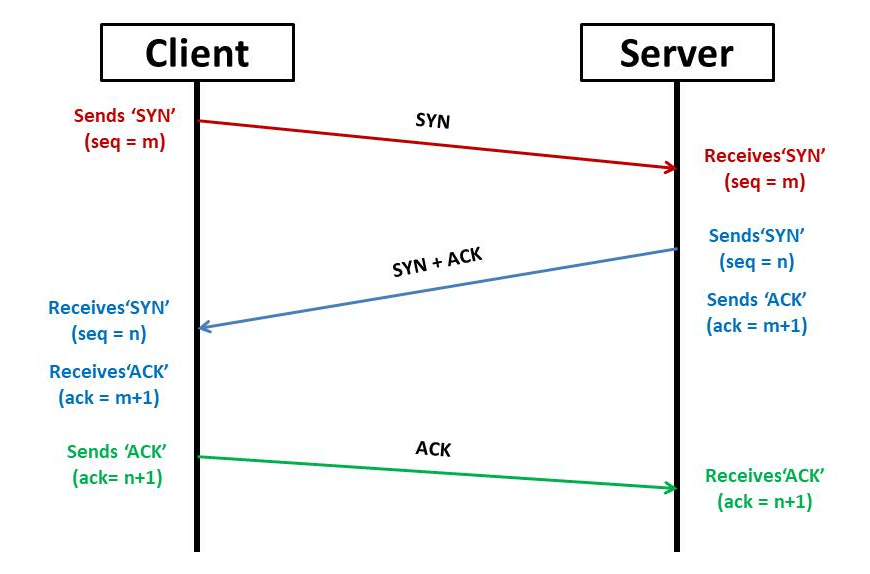
\includegraphics[width=0.75\linewidth]{./images/3wayhs.png}
    \caption{Three-way handshake}
\end{figure}

\newpage

\subsection{UDP - User Datagram Protocol}
È un protocollo minimal, scarno e \textit{unreliable}.

\begin{itemize}
    \item \textbf{Connectionless.}\\
    Non ha alcun tipo di handshake che stabilisca la connessione tra i due host.
    \item \textbf{Unreliable.}\\
    Nessuno scambio di ACK.
    \item \textbf{Nessun controllo del flusso.}\\
    UDP non gestisce il proprio throughput in funzione della congestione della rete, o del sovraccarico del receiver.
    \item \textbf{Nessuna garanzia sul throughput minimo.}    
\end{itemize}

UDP non è un protocollo sicuro: scopriremo però come il suo essere "ridotto all'osso", \textit{barebones}, sia il suo più grande punto di forza. È usato nei protocolli applicativi VoiP, streaming audio-video e gaming.


\newpage

\section{Telnet}
\textbf{Telnet} (da TErminaL NETwork) è un protocollo applicativo che permette di controllare il \textbf{terminale} di un altro host \textbf{da remoto}. 
\begin{figure}[htp]
    \centering
    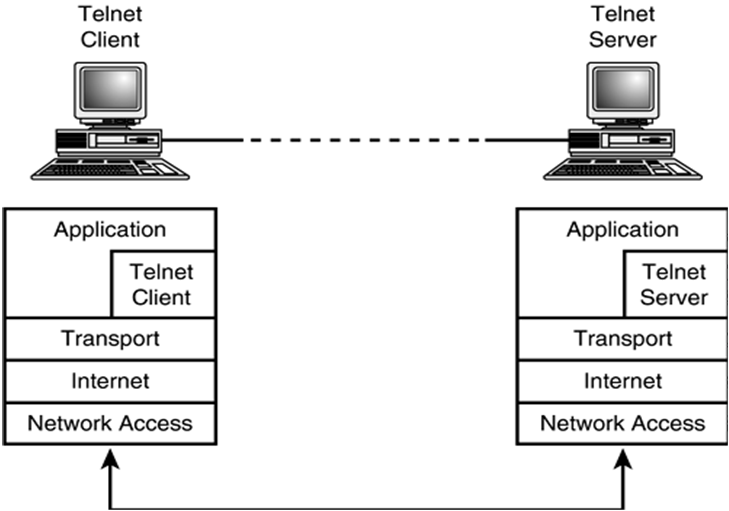
\includegraphics[width=0.5\linewidth]{./images/Requisiti di Telnet.png}
\end{figure}

È basato sul paradigma client-server (dove il pc remoto è il server), usa \textbf{TCP} la \textbf{porta 23} come porta destinataria (verso il server). 
Non è un protocollo sicuro: Telnet trasmette i dati (anche di autenticazione) in chiaro, l'autenticazione non è sempre obbligatoria, ed è vulnerabile a sniffing e man-in-the-middle. \textbf{SSH} (\textit{Secure Shell Protocol}) è simile al protocollo Telnet, ma sicuro, non trasmettendo i dati in chiaro. SSH usa la porta 22.

\subsection{Funzionamento di Telnet}
Basato sul protocollo di trasferimento TCP, Telnet sfrutta il three-way handshake per stabilire la connessione.
\begin{figure}[htp]
    \centering
    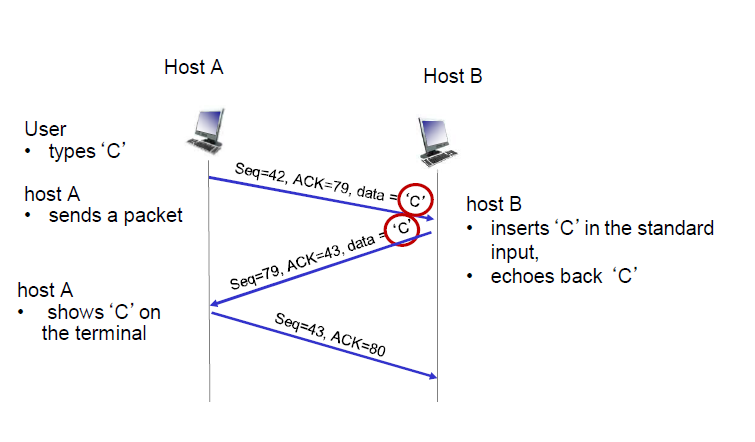
\includegraphics[width=0.75\linewidth]{./images/telnetscenario.png}
    \caption{Esempio di Telnet}
\end{figure}

Un fatto interessante è che Telnet può essere usato come strumento di debug per Server HTTP o Mail Server, inserendo come porta destinazione, una porta diversa dalla 23.


\subsection{Remote Desktop Protocol}
È un protocollo con presupposti simili a quelli di Telnet, ma che permette la trasmissione dell'intera interfaccia del dispositivo remoto.

\subsubsection{Telnet in breve}
Terminale remoto, TCP porta 23. Architettura client-server. Autenticazione trasmessa in chiaro, quindi non sicuro, sconsigliato e deprecato grazie ad SSH. SSH sfrutta la porta 22. 

\newpage

\section{FTP - File Transfer Protocol}
È un protocollo utilizzato per lo \textbf{scambio di file tra due host}. Basato sul paradigma \textbf{client-server}, sfrutta \textbf{TCP}. Offre inoltre un \textbf{meccanismo di autenticazione} (che avviene dopo lo stabilimento della connessione, ma precedentemente a qualsiasi scambio dati).

\subsection{Client-Server}
Col protocollo FTP, il client carica o scarica file verso o dal server. Il server ospita i file e gestisce le richieste.
La porta di controllo è la porta 21, su cui il server riceve le richieste. La porta del client usata per lo scambio dei dati è casuale, e trasmessa tramite il comando \verb|PORT|. La porta del server per lo scambio dati è la porta 20.

\begin{figure}[htp]
    \centering
    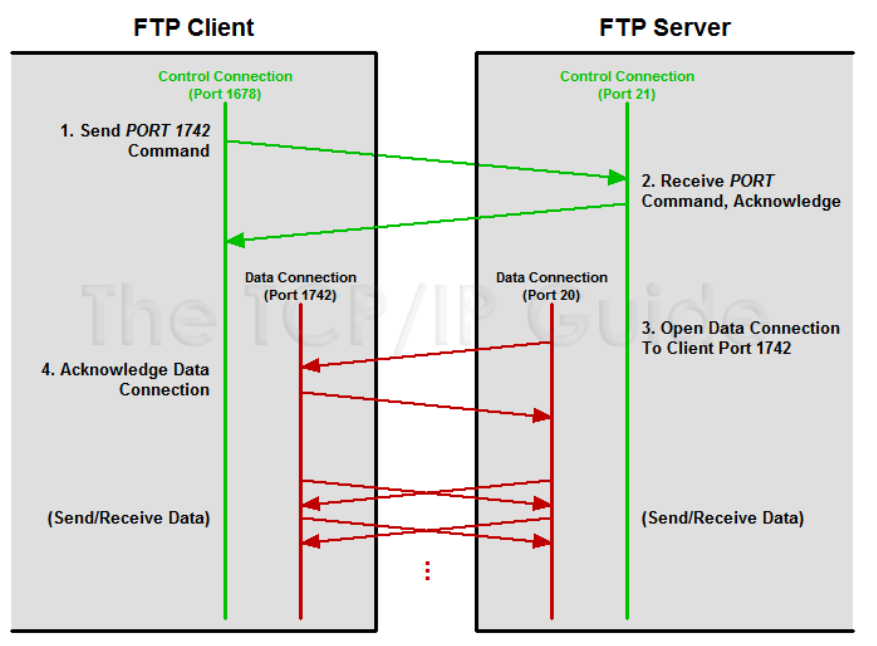
\includegraphics[width=0.75\linewidth]{./images/FTP.png}
    \caption{FTP}
\end{figure}

\subsection{Vulnerabilità del protocollo FTP}
\begin{itemize}
    \item Abilitare l'accesso all'intero file system tramite FTP è una mossa rischiosa: bisogna regolare quali porzioni rendere accessibili.
    \item Le credenziali di accesso e i dati (di default) sono trasmessi in chiaro, rendendo FTP vulnerabile ad attacchi man-in-the-middle e allo sniffing. Il protocollo \textbf{SFTP} risolve il problema implementando l'encryption di SSH. Usa la stessa porta di SSH, la porta 22.
\end{itemize}

\subsubsection{FTP in breve}
Upload e download di file su host remoto, TCP porta 21 (porta di controllo) e TCP porta 20 (porta dati) del server. Architettura client-server. Autenticazione e dati trasmessi in chiaro, quindi non sicuro, sconsigliato e deprecato grazie ad SFTP. SFTP sfrutta la porta di SSH, la porta 22. 

\newpage

\section{HTTP - HyperText Transfer Protocol}
\textbf{HTTP} permette ad un host di richiedere delle risorse, chiamate oggetti, ad un Web Server. Questi oggetti possono essere pagine HTML, file multimediali di vario tipo (e, col modello DHTML, affiancate alle pagine HTML, abbiamo anche fogli di stile CSS e file Javascript). Per accedere a queste risorse usiamo un URL (\textit{Uniform Resource Locator}). È quindi il protocollo alla base delle pagine Web, e segue (banalmente) l'architettura Client-Server.
La porta dedicata al protocollo, lato server, è la porta 80, ed è la porta da cui il server riceverà le richieste. Ricordiamo che la porta sorgente del client è stabilita (casualmente) dall'OS.

\begin{figure}[htp]
    \centering
    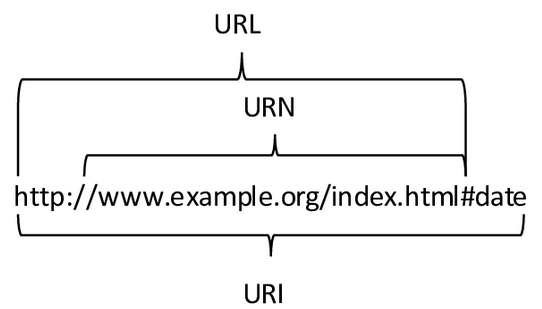
\includegraphics[width=0.6\linewidth]{./images/URL.png}
\end{figure}

\subsection{In cosa consiste la connessione HTTP}
HTTP utilizza TCP e il suo Three-Way Handshake.
\begin{enumerate}
    \item Il client \textbf{richiede la connessione TCP sulla porta 80} del server.
    \item Il \textbf{server accetta} la connessione TCP da parte del client.
    \item \textbf{Messaggi HTTP vengono scambiati} tra il browser (del client) e il web server (del server).
    \item \textbf{Si chiude la connessione} TCP.
\end{enumerate}

Questi passi avvengono in un tempo chiamato \textit{Round Trip Time (RTT)}.

\subsection{Versioni di HTTP}
Il vasto utilizzo di HTTP, ha portato alla creazione di molteplici versioni nel corso degli anni.
\begin{itemize}
    \item \textbf{HTTP/1.0}\\
    Ogni trasferimento di oggetto implica un'apertura e chiusura di una connessione TCP. \textbf{Per ogni oggetto, una connessione TCP dedicata}. Overhead per ogni oggetto.
    \item \textbf{HTTP/1.1}\\
    Usa una \textbf{connessione TCP persistente}. La connessione viene \textbf{aperta all'inizio del trasferimento} di tutti gli oggetti, e \textbf{chiusa alla fine}. Meno overhead, ma ogni download avviene in maniera sequenziale.
    \item \textbf{HTTP/2}\\
    Comprime gli header e effettua i download in parallelo. Riduce ulteriormente le tempistiche.
    \item \textbf{HTTP/3}\\
    Il più recente, introduce numerose innovazioni, tra cui l'uso del protocollo di trasferimento QUIC (creato su UDP!).
\end{itemize}

\subsubsection{HOL Blocking}
L'\textbf{Head-of-Line blocking} è un fenomeno che avviene quando più richieste di risorse HTTP sono in coda. In HTTP/1.1, se $O_1$, una richiesta di un oggetto molto grande, viene inserita prima della richiesta di 3 oggetti molto piccoli $O_2,O_3,O_4$, la priorità verrà data all'oggetto $O_1$, in quanto quest'ultimo è situato in testa.
In HTTP/2, un insieme di algoritmi di \textbf{valutazione della priorità} e \textbf{slicing} degli oggetti in porzioni più piccole, risolve l'HOL blocking minimizzando i tempi di attesa per ogni oggetto, migliorando la \textit{User Experience}.

\newpage

\subsection{Struttura di una richiesta HTTP}

\begin{itemize}
    
    \item \textbf{Request Line.}
    \begin{itemize}
    \item \textbf{Metodo.}\\
    Indica il tipo di richiesta effettuata dal client.
    \item \textbf{URL.}\\
    Esplicita la risorsa desiderata.
    \item \textbf{Versione.}
    Esplicita la versione del protocollo HTTP.
    \end{itemize}

    
    \item \textbf{Header lines.}\\
    Più righe contenenti coppie \verb|Nome campo: Valore|, una per riga.
    \item \textbf{Body.}\\
    Che permette di specificare ulteriori parametri.
\end{itemize}

\begin{figure}[htp]
    \centering
    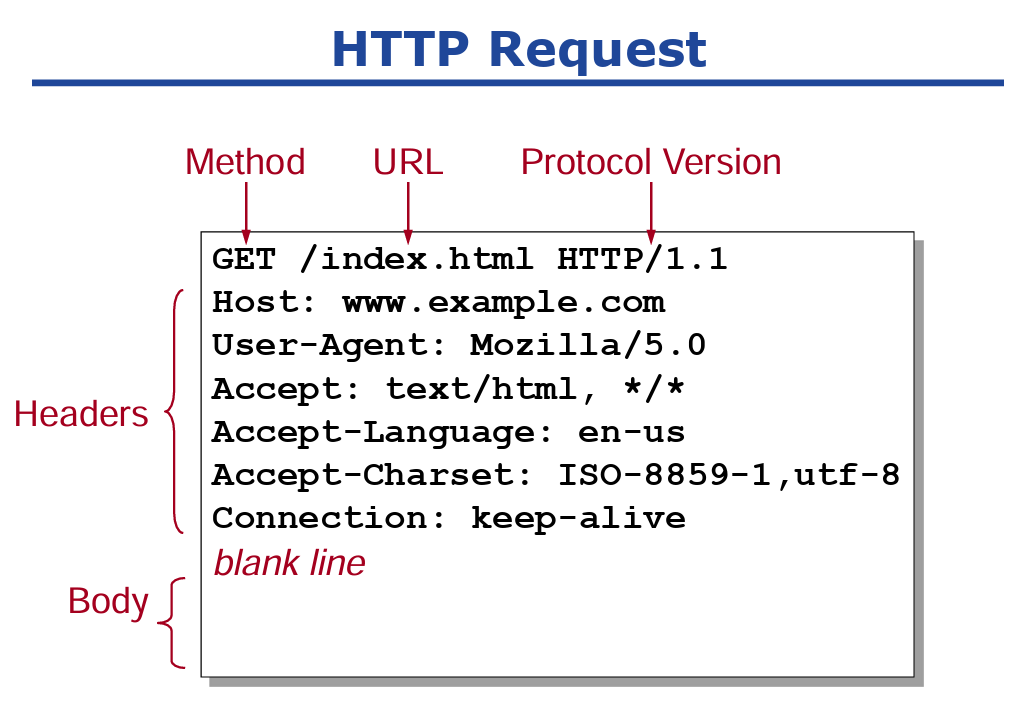
\includegraphics[width=0.75\linewidth]{./images/richiestahttp.png}
    \caption{Esempio di richiesta HTTP}
\end{figure}

\subsubsection{Alcuni metodi richieste HTTP}

\begin{itemize}
    \item \verb|GET|.\\
    Richiede dei dati dal server.
    \item \verb|POST|.\\
    Usato per mandare dei dati d'input da un client.
    \item \verb|HEAD|.\\
    Richiede esclusivamente l'header che sarebbe mandato da una richiesta HTTP \verb|GET| ad un determinato URL.
    \item \verb|PUT|.\\
    Usato per effettuare l'upload dei dati. Effettua un rimpiazzamento totale di un file che esiste a un determinato URL.
\end{itemize}

\newpage

\subsection{Struttura di una risposta HTTP}

\begin{itemize}
    
    \item \textbf{Status Line.}
    \begin{itemize}
    \item \textbf{Versione.}\\
    Ribadisce la versione del protocollo HTTP in uso.
    \item \textbf{Codice di stato.}\\
    Fornisce dettagli sulla corretta (o meno) elaborazione di una richiesta HTTP.
    \item \textbf{Messaggio di stato.}
    Esprime in linguaggio naturale il significato dello Status Code.
    \end{itemize}

    \item \textbf{Header lines.}\\
    Più righe contenenti coppie \verb|Nome campo: Valore|, una per riga.
    \item \textbf{Body.}\\
    Contiene i dati richiesti dal client nella rispettiva HTTP Request.
\end{itemize}

\begin{figure}[htp]
    \centering
    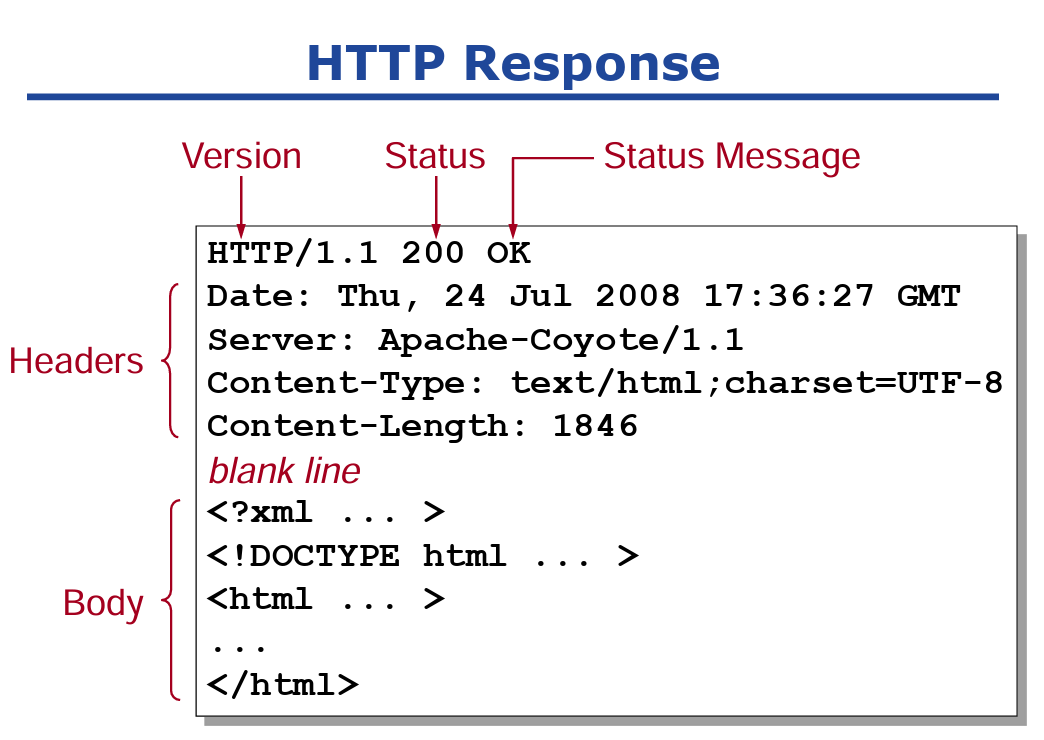
\includegraphics[width=0.75\linewidth]{./images/rispostahttp.png}
    \caption{Esempio di risposta HTTP}
\end{figure}


\subsubsection{Alcuni codici di risposta HTTP}
\begin{verbatim}
Information codes.
   100 Continue
   Success codes.
   200 OK
   203 Non-Authorative Information
   204 No Content
   
Redirection Codes.
   305 Use Proxy
   
Client Error Codes.
   400 Bad Request
   403 Forbidden
   404 Not Found
   405 Method Not Allowed
   
Server Error Codes.
   500 Internal Server Error
   505 HTTP Version Not Supported
\end{verbatim}

\newpage

\subsection{Parentesi Stateless, Stateful e Cookies}
Il protocollo HTTP è di default, un protocollo di tipo \textbf{stateless}. Tuttavia, con l'introduzione dei \textbf{cookies}, HTTP può memorizzare degli stati, diventando \textbf{stateful}\footnote{Un protocollo stateless può comunque avere un log delle azioni relative alle sessioni precedenti, ma ciò non cambierà il suo comportamento. Un web-server PHP hostato con Apache non diventa magicamente stateful se aggiungiamo un log. Rettifica importante, soprattutto in sede d'esame.}.

\begin{itemize}
    \item \textbf{Stateless.}\\
    Il comportamento di un protocollo stateless \textbf{non cambia in funzione} di \textbf{stati intermedi} della \textbf{attuale sessione} e delle \textbf{sessioni precedenti}. 
    \item \textbf{Stateful.}\\
    Un protocollo stateful \textbf{salva informazioni} relative a stati intermedi e richieste precedenti, \textbf{costruendo uno storico degli stati}, e il suo comportamento varia. Un crash del server potrebbe portare a storici di attività e stati inconsistenti. In tal caso, bisognerà ricostruire lo storico. Tra i due tipi di protocolli, questo è il più complesso da gestire.
\end{itemize}

\subsection{I cookies}
Permettono ad un server associato al Web Server di memorizzare alcuni dei dati relativi alle sessioni dell'utente che li accetta.
Una volta che un utente accetta i cookies su una piattaforma, viene creato un record (con chiave primaria uguale al cookie id) in un database back-end relativo al sito, che può essere quello del sito stesso o meno. I cookies permettono di implementare \textbf{carrelli online} e \textbf{accesso semplificato} all'interno di pagine web. Nel pratico, i cookies sono dei veri e propri file gestiti dal proprio web browser.

\begin{figure}[htp]
    \centering
    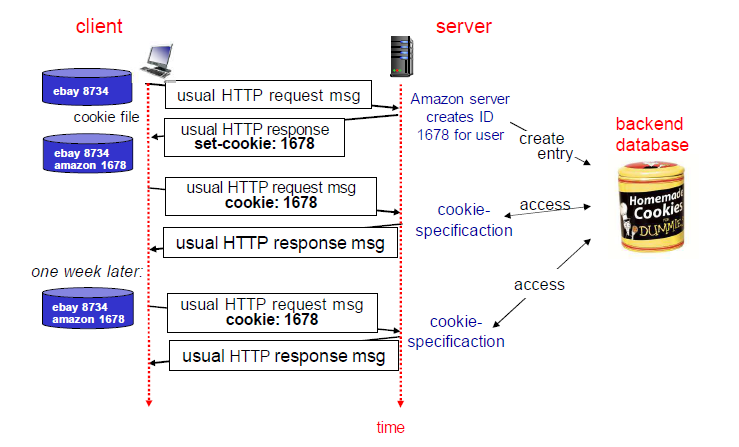
\includegraphics[width=0.75\linewidth]{./images/biscotti.png}
\end{figure}

\subsubsection{I cookies - rappresentano un rischio per la privacy degli utenti?}
Seppur apparentemente convenienti, i cookies sono in tutto e per tutto \textbf{un rischio per la privacy} degli utenti che li accettano. In particolare, se i \textbf{cookie di prima parte} tracciano azioni dell'utente solo sul sito da esso visitato, i tanto sentiti \textbf{cookie di terze parti} permettono di tracciare le azioni degli utenti anche a siti \textbf{non visitati in maniera diretta}, ma semplicemente in quanto embedded in altri siti.

\begin{enumerate}
    \item \verb|GET| da parte del client ad un sito $A$: cookie di terze parti vengono accettati.
    \item Le informazioni prese dal cookie del sito $A$ vengono prelevate anche da siti di terze parti (integrati nella pagina, embedded), e quindi finiscono anche nel database back-end di un sito $B$.
    \item Supponiamo il sito esterno sia embedded in un altro sito $C$. Se lo stesso client è che ha visitato il sito $A$, visiterà anche il sito $C$, il sito $B$ otterrà entrambe le informazioni, potendo effettivamente costruire uno storico dell'attività dell'utente.
\end{enumerate}

Gli utenti e le loro attività online, possono essere tracciate, soprattutto se ai cookies associamo meccanismi di identificazione univoci! Il \textbf{Regolamento Generale sulla Protezione dei Dati} stabilisce e regolamenta l'integrazione dei cookies nei siti web, garantendo che i cookies \textit{analytics} e non essenziali (non-tecnici) possano essere bloccati.

\begin{figure}[htp]
    \centering
    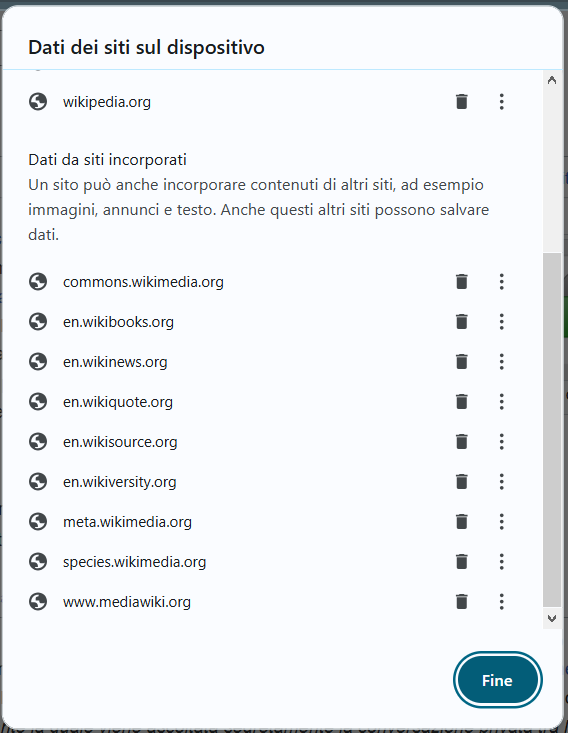
\includegraphics[width=0.5\linewidth]{./images/embeddedcookies.png}
    \caption{Cookies di pagine embedded a wikipedia.org}
\end{figure}
\subsection{DHTML}
È possibile anche costruire una pagina web dinamica col Dynamic HTML: è un insieme di tecnologie che permettono di costruire pagine web con rendering dinamico in funzione dell'utente. Queste tecnologie includono JavaScript e fogli di stile CSS.

\subsubsection{HTTP in breve}
HyperText Transfer Protocol permette agli host di richiedere oggetti (pagine HTML, media e altro) ad un Web Server, e al Web server di rispondere, tramite opportune richieste e risposte HTTP. Usa TCP (sfruttato in maniera differente tra le varie versioni di HTTP), sulla porta 80 del server. Architettura client-server. È stateless, ma possono essere annesse funzionalità stateful tramite l'ausilio di cookies, con i pro e contro del caso. 


\section{Server proxy}
È un server intermedio che permette di \textbf{controllare}, \textbf{filtrare} e \textbf{mascherare il traffico} da parte di uno o più client. Nello specifico:
\begin{enumerate}
    \item I client mandano le richieste al proxy.
    \item Il proxy le invia al server destinazione.
    \item Il server riceve la richiesta del proxy.
    \item Il server invia la risposta al proxy.
    \item Il proxy invia la risposta del server al client originale.
\end{enumerate}

I proxy server si prestano alla perfezione per mascherare IP e monitorare le richieste da parte degli host che li usano.
\newpage

\section{SMTP}
Il \textbf{Simple Mail Transfer Protocol} è un protocollo di invio di e-mail. Si occupa del trasferimento dei messaggi dal mail server del mittente a quello del destinatario.
Usa il protocollo \textbf{TCP} e sulla \textbf{porta 25}.

\begin{itemize}
    \item \textbf{User Agent}.\\
    Software che permette agli utenti di leggere, rispondere, inoltrare, salvare e comporre messaggi. Sono i comuni Microsoft Outlook, Apple Mail, Google Gmail. Permettono di inserire o leggere messaggi sul mail server.
    \item \textbf{Mail Server}.\\
    È il server di posta da cui vengono recuperati, prelevati e inviati i messaggi. Se i due client non sono connessi allo stesso mail server, allora avviene un trasferimento tra i due mail server.
\end{itemize}

\subsection{Le tre fasi di SMTP}
\begin{enumerate}
    \item \textbf{Handshaking.}\\
    Connessione alla \textbf{porta 25} del mail server, il client si identifica tramite il comando \verb|HELO|, il server invia un messaggio di benvenuto.
    
    \item \textbf{Transfer of messages.}\\
    \verb|> MAIL FROM: <indirizzo@email.com>| per specificare email del mittente. \\
    \verb|> RCPT TO: <destinatario@email.it>| per specificare i destinatari. \\
    \verb|> DATA| per iniziare a scrivere la propria mail. Si può andare a capo, una mail si chiude con una riga con esclusivamente il carattere "\verb|.|".
    Si può ripetere questo passaggio per scrivere più mail: queste verranno mandate tutte assieme con la \textbf{stessa sessione TCP} persistente.
    
    \item \textbf{Closure.}\\
    \verb|> QUIT|. Viene chiusa la connessione.
\end{enumerate}


\begin{table}[htp]
    \centering
    \begin{tabular}{|c|p{9cm}|}
        \hline
        \textbf{Header} & \textbf{Significato}\\
        \hline
        \cellcolor{blue!25}To: & Indirizzi e-mail dei destinatari primari\\
        \hline
        Cc: & Indirizzi e-mail dei destinatari secondari\\
        \hline
        Bcc: & Come Cc: ma gli indirizzi e-mail non sono visibili\\
        \hline
        \cellcolor{blue!25}From: & Indirizzo e-mail di chi ha scritto il messaggio\\
        \hline
        Sender: & Indirizzo e-mail dell'effettivo mittente\\
        \hline
        Received: & Ogni server attraverso cui passa la mail lascia
        una traccia in questo campo\\
        \hline
        Return Path: & Può identificare un cammino a ritroso verso il mittente\\
        \hline
        Date: & Data e ora di invio\\
        \hline
        Reply-to: & Indirizzo e-mail a cui le risposte dovrebbero essere inviate\\
        \hline
        Message-id: & Id univoco del messaggio\\
        \hline
        In-Reply-To:& Id del messaggio a cui si è risposto\\
        \hline
        References: & Altri id di messaggi\\
        \hline
        Keywords: & Parole chiave scelte dall'utente\\
        \hline
        \cellcolor{blue!25} Subject: & Breve riepilogo del contenuto del messaggio\\
        \hline
    \end{tabular}
    \caption{Tutti gli header dell'SMTP. In blu, i campi obbligatori}
\end{table}

\subsubsection{Sugli allegati}
Gli \textbf{allegati} delle e-mail sono trasferiti tramite il protocollo \textbf{MIME} (Multipurpose Internet Mail Extension).

\newpage

\subsection{Protocolli del mail server - POP3 e IMAP}
Erroneamente, si potrebbe pensare che il Mail Server giri localmente all'interno della macchina dell'utente. Tuttavia, questo obbligherebbe ogni utente a tenere il proprio dispositivo sempre acceso e in ascolto sulla rete, per assicurare che non venga persa alcuna mail: il server non sarebbe sempre attivo, caratteristica che nel paradigma client-server è fondamentale. Deleghiamo quindi la gestione del \textit{pull} delle e-mail dal Mail Server a dei protocolli, riservando il \textit{push} al protocollo SMTP.

\begin{itemize}
    \item \textbf{IMAP.}\\
    Internet Message Access Protocol. Memorizza le e-mail sul mail server. Questo permette l'accesso alle stesse e-mail da più dispositivi, e grava meno sulla memoria. Usa TCP sulla porta 143 (non crittografata) e 993 (crittografata).
    \item \textbf{POP3.}\\
    Post Office Protocol. Memorizza le e-mail in locale sulla macchina dell'utente, rimuovendole dal Mail Server, non supportando la sincronizzazione delle e-mail su più dispositivi. Usa TCP sulla porta 110 (non crittografata) e 995 (crittografata).
\end{itemize}

\begin{figure}[htp]
    \centering
    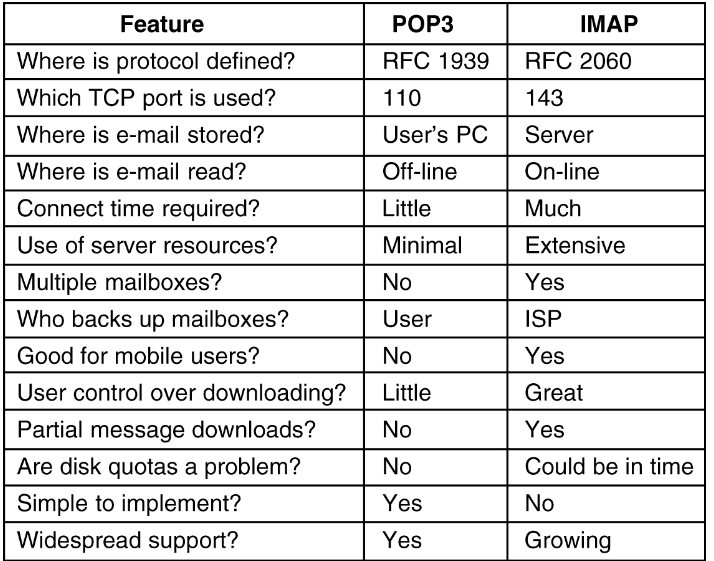
\includegraphics[width=0.75\linewidth]{./images/pop3imap.png}
    \caption{Protocolli POP3 e IMAP a confronto}
\end{figure}

\subsubsection{SMTP, POP3 e IMAP in breve}
\begin{itemize}
    \item \textbf{Simple Mail Transfer Protocol} offre modo al client di mandare, \textit{pushare}, email ad un Mail Server. Usa TCP sulla porta 25 del mail server.
    \item \textbf{Postal Office Protocol} (POP3) permette al client di scaricare, \textit{pullare}, in locale le proprie e-mail, ma solo su un dispositivo. Nel mail server non rimarrà traccia di email che sono state prelevate con questo protocollo. Usa TCP sulla porta 110 del mail server.
    \item \textbf{Internet Message Access Protocol} (IMAP) permette al client di accedere alle e-mail presenti nella propria casella postale del mail server. Non grava sulla memoria del dispositivo, e permette l'accesso da più dispositivi. Usa TCP sulla porta 143 del mail server.
\end{itemize}
\newpage

\section{DNS - Domain Name System}
Gli indirizzi \textbf{IP} \textbf{identificano in maniera univoca gli host in rete} e la loro locazione: la struttura di un indirizzo IP, fornisce infatti informazioni sulla struttura della (sotto)rete e la \textbf{posizione dell'host} all'interno di essa. 
Gli IP \textbf{non sono facili da ricordare}, per un umano, in quanto costituiti esclusivamente da \textbf{caratteri numerici}. Gli \textit{hostname} nascono con lo scopo di associare \textbf{un nome a un IP}: diventa però necessario introdurre un meccanismo che permetta la traduzione degli hostname in indirizzi IP. Nasce così il DNS.
\begin{verbatim}
        151.97.240.12   <-   www.dmi.unict.it
        151.97.240.4    <-   www.unict.it
        151.97.6.236    <-   www.ing.unict.it
        151.97.252.132  <-   galileo.dmi.unict.it
\end{verbatim}

Il protocollo DNS supporta inoltre:
\begin{itemize}
    \item \textbf{Alias names} sugli hostname canonici. 
    \item Gestione dei reindirizzamenti nel caso di cambio di indirizzo IP del sito.
    \item Distribuzione del carico su più server (tra server DNS primari e secondari).
\end{itemize}

\subsection{DNS - Transport Layer}
Le richieste \textbf{sono mandate} alla \textbf{porta 53} dei server DNS. Il protocollo usa \textbf{sia UDP}, che \textbf{TCP}. Per le banali query del servizio, si predilige UDP, e TCP è riservato per risolvere circostanze particolari, come informazioni troncate.
TCP è sempre usato durante gli \textbf{zone transfer}, ossia quando un DNS primario vuole effettuare una copia dei suoi record ad uno o più server DNS secondari.

\subsection{Struttura del DNS}
È un \textbf{database distribuito}, con una \textbf{struttura gerarchica} ad albero che \textbf{velocizza la ricerca dell'IP}.\\
Individuiamo le classi di DNS della gerarchia:

\begin{itemize}
    \item \textbf{Root server.}\\
    Contengono gli indirizzi IP del TLD server. I root server sono 13, gestiti da 12 aziende, e nel complesso si hanno più di 1000 copie di questi record.
    \item \textbf{Top-Level Domain Server.}\\
    Si occupano degli indirizzi IP dei server autoritativi, e sono organizzati per domini di primo (\verb|.com .gov .org .net .edu|) e di secondo livello (\verb|.it .uk .us|).

    \item \textbf{Authoritative Domain Name Server.}\\
    Effettuano l'ultima associazione indirizzo IP - hostname.
\end{itemize}

Su questa struttura gerarchica, aggiungiamo anche una \textbf{distribuzione del carico di lavoro} tra più server (\textbf{primari} e \textbf{secondari}), \textbf{meccanismi di caching} vari e \textbf{distribuzione di questi server a scala mondiale}: questi fattori rendono il DNS uno dei servizi più \textbf{robusti} (gestione non centralizzata), \textbf{affidabili} e \textbf{veloci} della rete.

\begin{figure}[htp]
    \centering
    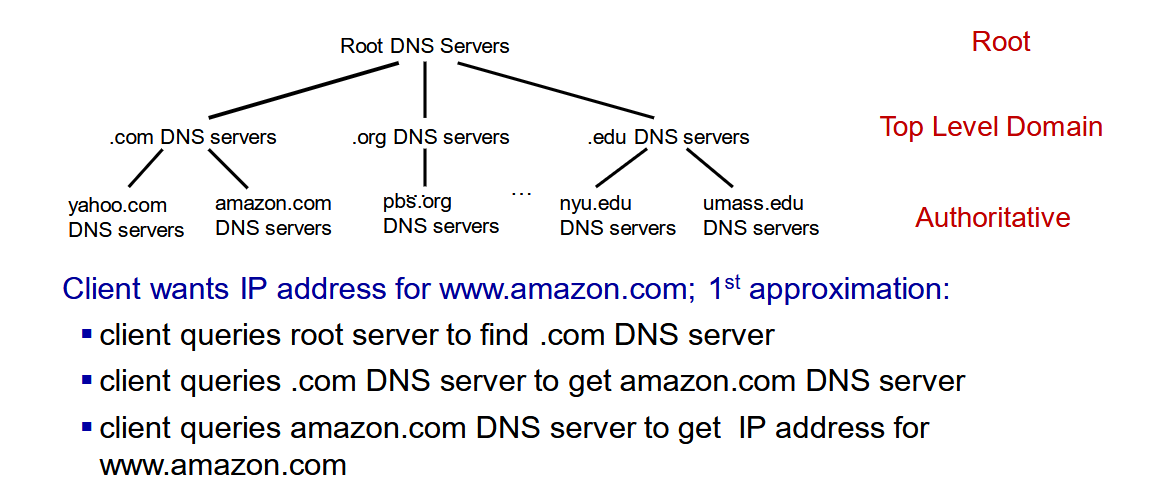
\includegraphics[width=0.75\linewidth]{./images/gerarchiadns.png}
\end{figure}

\subsection{Primary e secondary DNS}
A causa dell'\textbf{alto numero di richieste} ai server DNS, \textbf{a ogni DNS primario}, contenente le copie originali dei record in modalità lettura e scrittura, \textbf{coincidono molteplici DNS secondari}, contenenti \textbf{copie di sola lettura}. Lo scopo è quello di \textbf{bilanciare il carico} di lavoro tra i DNS.



\subsection{Name resolution - Modo iterativo}
\begin{figure}[htp]
    \centering
    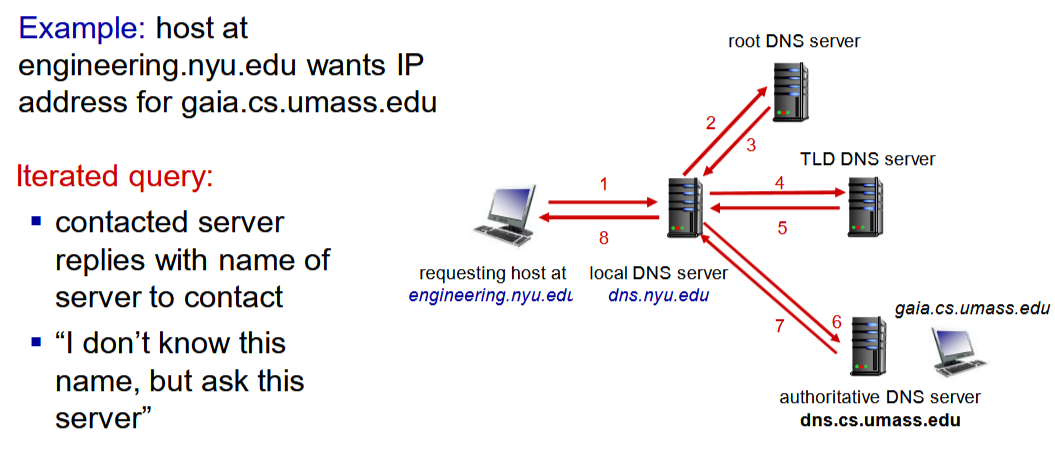
\includegraphics[width=0.75\linewidth]{./images/iterative.png}
\end{figure}

Le query iterative offrono una strategia di controllo che \textbf{distribuisce bene il carico} sui vari server. Tuttavia, il client dovrà gestire molte più richieste, una per DNS coinvolto. (N.B. la prima query dell'immagine è ricorsiva!)

\subsection{Name resolution - Modo ricorsivo}
\begin{figure}[htp]
    \centering
    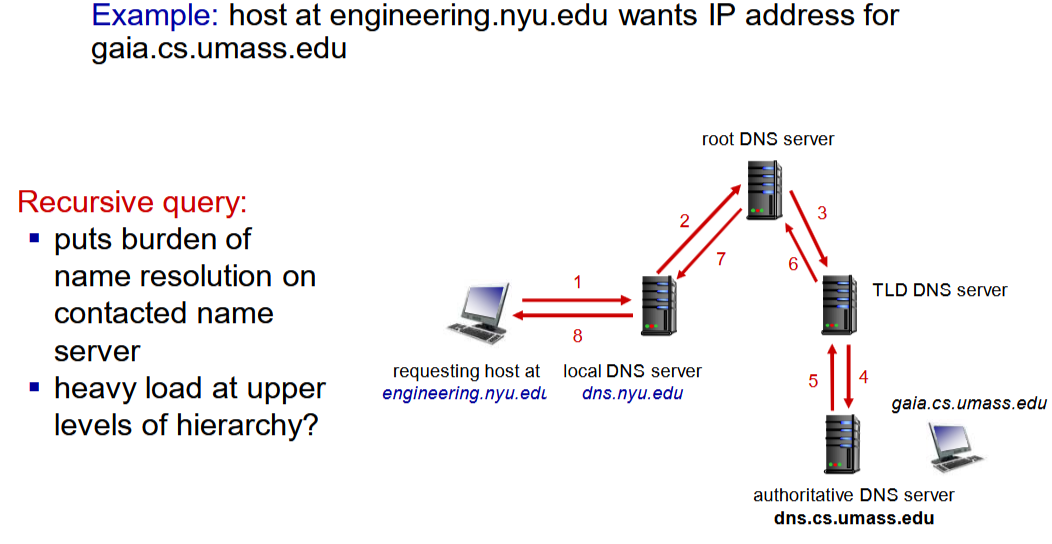
\includegraphics[width=0.75\linewidth]{./images/recur.png}
\end{figure}

Le query ricorsive offrono una \textbf{risposta diretta} al client \textbf{senza ulteriori richieste} da mandare. Ogni server comunicherà con quello successivo e quello precedente (\textbf{favorendo il caching}, i server DNS si scambieranno le loro risposte), con una logica molto più semplice di quella iterativa. Tuttavia, a causa della ricorsione, si avrà \textbf{maggiore latenza} (soprattutto quando non avvengono cache hit), e \textbf{maggior carico di lavoro} sulla parte alta della gerarchia dei server DNS. 

\subsection{Caching e Updating DNS}
Ogni volta che un qualunque DNS Server (name server) riceve una risposta e “impara” come mappare una determinata informazione, la \textbf{memorizza nella propria cache} per evitare future richieste nella gerarchia di risoluzione. Ciò permette di ridurre il carico sui server e migliorare le prestazioni. Tipicamente, i TLD server vengono memorizzati nella cache dei DNS locali per ridurre le query ai root. Le entry delle cache (anche quelle locali) devono essere \textbf{aggiornate periodicamente} dopo un tempo identificato dal \textbf{TTL} (Time To Live): esso è un valore associato ai record DNS che indica per quanto tempo un resolver DNS \textbf{può mantenere nella cache una risposta prima di doverla aggiornare}. Il caching velocizza significativamente il funzionamento dei DNS. Un cache hit eviterà la richieste a tutti DNS server dei livelli inferiori della gerarchia: per questo la cache di ciascun DNS è il \textbf{primo elemento che viene consultato per qualsiasi richiesta}. Una cache hit è sempre un grande vantaggio in termini di velocità.

\newpage

\subsection{Forma di un record di un DNS}
\begin{verbatim}
RR format: (name, value, type, ttl)
\end{verbatim}
\begin{itemize}
    \item type=A:\\
    \verb|name| è l'hostname, \verb|value| è l'IP address
    
    \item type=NS:\\
    \verb|name| è il dominio, \verb|value| è l'hostname del server autoritativo su questo dominio.
    
    \item type=CNAME\\
    Canonical Name. \verb|name| è un alias per il nome canonico \verb|value|.

    \item type=MX\\
    \verb|value| è il nome del mail server associato all'hostname \verb|name|.
\end{itemize}

\subsection{Forma di un messaggio DNS}
Formato uguale tra query e risposte.
\begin{figure}[htp]
    \centering
    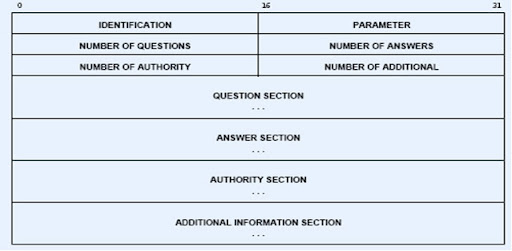
\includegraphics[width=1\linewidth]{./images/dnsmex.png}
\end{figure}

\begin{itemize}
    \item \textbf{Sezione di intestazione.}\\
    Sono i primi 12 byte, e contiene vari campi.
    \begin{itemize}
        \item Identificazione, 16 bit. Permette di associare risposte a richieste.
        \item Flag, 16 bit. Tra questi, un bit che specifica \verb|query/reply|.
        \item Numero di domande, numero record di risposta, numero record autoritativi, numero record addizionali.
        Specificano il numero di record e domande delle prossime sezioni. Ognuno è un numero a 16 bit.
    \end{itemize}

    \item \textbf{Sezione delle domande.}\\
    Include informazioni relative alle richieste che stanno per essere effettuate, un campo con il nome richiesto e uno con il tipo di domanda sul nome richiesto.

    \item \textbf{Sezione delle risposte.}\\
    Presente nei messaggi di risposta. I record contengono al loro interno le informazioni specificate nel paragrafo precedente. Una risposta può tornare più indirizzi.

    \item \textbf{Sezione autoritativa.}\\
    Contiene record di altri server autoritativi.

    \item \textbf{Sezione aggiuntiva.}\\
    Contiene altri record utili correlati alla richiesta.
\end{itemize}

\newpage

\subsection{nslookup}
Questo programma permette di effettuare richieste DNS a un determinato dominio.
\begin{verbatim}
> nslookup
Server predefinito:  vodafone.station
Address:  **indirizzo mac**

> wikipedia.com
Server:  vodafone.station
Address:  **indirizzo mac**

Risposta da un server non autorevole:
Nome:    wikipedia.com
Addresses:  2a02:ec80:600:ed1a::3           //IPv6
          185.15.58.226                     //IPv4

> overleaf.com
Server:  vodafone.station
Address:  **indirizzo mac**

Risposta da un server non autorevole:
Nome:    overleaf.com
Address:  34.120.52.64                  

> overleaf.it
Server:  vodafone.station
Address:  **indirizzo mac**

*** vodafone.station non è in grado di trovare overleaf.it: Non-existent domain
\end{verbatim}

\subsection{Problemi di sicurezza e criticità dei DNS}
\begin{itemize}
    \item \textbf{DDoS attacks su Root Server}.\\
    Consiste nel sovraccaricamento di un DNS root tramite richieste spazzatura. Il traffic filtering può essere una soluzione per filtrare il traffico osservando la semantica degli URL. Questo approccio potrebbe rifiutare richieste da utenti reali. Al giorno d'oggi, a questo scopo, vengono sfruttate alcune tecniche d'intelligenza artificiale.
    Un'altra soluzione può essere mantenere una lista di IP di TLD server notoriamente non malevoli.
    
    \item \textbf{Man-in-the-middle}.\\
    Un attacco che consiste nell'intercettare le richieste tra i DNS.
    
    \item \textbf{DNS poisoning/DNS spoofing}.\\
    Consiste nel sostituire risposte DNS effettive con risposte fittizie, ottenendo un \textbf{reindirizzamento errato}. I danni da DNS poisoning si propagano \textbf{a lungo termine}, a causa del \textbf{caching}.
\end{itemize}

\subsubsection{DNS in breve}
Risoluzione degli hostname in indirizzi IP. UDP (ma anche TCP), porta 53 del server ricevente. Architettura client-server. Sfrutta un sistema di server distribuiti, e organizzati in maniera gerarchica, per facilitare la ricerca. Meccanismi di caching, distribuzione del carico su server primari e secondari, e in generale l'alto numero di server nel mondo, offrondo un sistema solido e veloce.

\newpage

\section{SNMP}
Il \textbf{Simple Network Management Protocol} è un protocollo di rete \textbf{connectionless} che permette la \textbf{gestione di una rete} e il \textbf{monitoraggio dei dispositivi} ad essa collegati. Gli \textbf{amministratori} possono raccogliere informazioni sulle prestazioni e lo stato dei dispositivi.

\subsection{Attori del SNMP}
\begin{itemize}
    \item \textbf{Manager SNMP.}\\
    Applicazione che comunica con i dispositivi della rete, per raccogliere informazioni. Può inviare richieste agli agenti SNMP.
    
    \item \textbf{Agente SNMP.}\\
    È un software presente in ogni dispositivo della rete da monitorare. Raccoglie informazioni relativi al dispositivo (quali stato, configurazione, prestazioni, etc.) e risponde alle richieste del manager con queste informazioni.
    
    \item \textbf{MIB (Management Information Base).}\\
    È un database, presente in ogni agente SNMP, che definisce le informazioni che possono essere raccolte o modificare tramite SNMP.
    
    \item \textbf{Protocollo SNMP.}\\
    È il protocollo vero e proprio utilizzato nella comunicazione tra agenti e manager. È basato sul paradigma client-server. Il manager è il client, l'agente fa da server.
\end{itemize}
Usa il protocollo \textbf{UDP} e la\textbf{porta 161} degli agenti per mandare messaggi, e la \textbf{porta 162} del manager per ricevere le \textbf{notifiche} (\textit{traps}).\\
Le \textbf{traps} sono generate successivamente a \textbf{malfunzionamenti, eventi e anomalie}.

\subsection{Messaggi SNMP}
\subsubsection{Da manager a agente}
\begin{itemize}
    \item \verb|GetRequest|.\\
    Richiesta di recupero del valore di una variabile.
    \item \verb|SetRequest|.\\
    Richiesta di cambiamento del valore di una variabile.
    \item \verb|GetNextRequest|.\\
    Richiesta di recupero di possibili variabili e dei loro valori.
\end{itemize}

\subsubsection{Da agente a manager}
\begin{itemize}
    \item \verb|GetResponse|.\\
    Restituisce il valore di una o più variabili.
    \item \verb|Trap|.\\
    Notifica in maniera asincrona e senza richiesta del manager situazioni anomale o eventi significativi della rete.
\end{itemize}

\subsection{Versioni di SNMP}
La prima versione di SNMP presentava numerose criticità in termini di sicurezza e performance migliorabili. La seconda e la terza versione migliorano la sicurezza del protocollo, le performance. In particolare con la terza versione, viene introdotta la crittografia per i dati e un sistema di autenticazione.

\subsubsection{SNMP in breve}
\textbf{Simple Network Management Protocol} offre un servizio per la gestione. UDP, \textbf{porta 161 degli agenti}, \textbf{porta 162 del manager}. Architettura client-server: i server sono gli agenti. Ogni dispositivo agente ha una base di dati contenente oggetti per gestire i dispositivi di rete e i loro attributi. I dispositivi possono segnalare anomalie al manager tramite delle traps. È un protocollo \textbf{connectionless} con \textbf{comunicazioni asincrone}.


\chapter{Transport Layer}

\section{Introduzione al Transport Layer}
Il transport layer è situato tra l'application e il network layer. I protocolli di questo livello, permettono all'application layer di usufruire di una \textbf{connessione logica tra processi}, e quindi di una comunicazione \textbf{end-to-end}. 

\subsection{Connessione logico, connessione reale}
Introducendo il concetto di \textbf{protocollo}, abbiamo capito che questi forniscono delle specifiche di "incapsulamento" e delle specifiche di "interpretazione" dei dati. Inoltre, abbiamo capito che in termini esclusivamente \textbf{logici}.,  l'$i$-esimo layer di un host $A$, comunica direttamente con l'$i$-esimo layer dell'host $B$. $A$ incapsula i dati con header opportuni, $B$ interpreta in maniera opportuna seguendo le indicazioni del protocollo e degli header.\\
Ogni layer ha un ruolo specifico, in particolare:
\begin{itemize}
	\item Il \textbf{livello di trasporto} crea una \textbf{connessione logica tra processi}.
	\item Il \textbf{livello di rete}, crea una \textbf{connessione logica tra host}.
	\item Il \textbf{livello di collegamento} (Data Link) si occupa della \textbf{comunicazione fisica} tra due host (fisicamente) collegati.
\end{itemize}

\begin{figure}[htp]
	\centering
	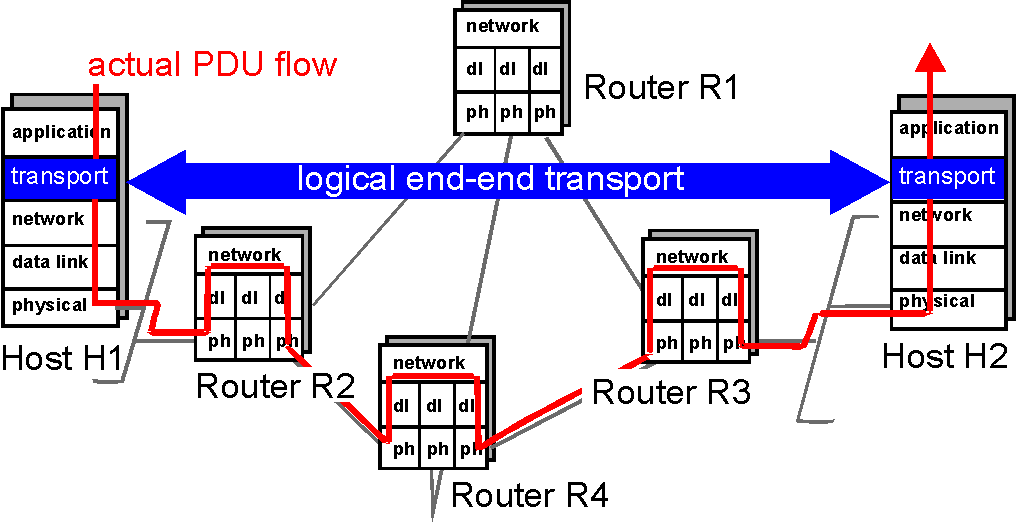
\includegraphics[width=0.75\linewidth]{./images/connessione.png}
	\caption{Trasferimento logico vs effettivo}
\end{figure}

\newpage

Nonostante la comunicazione \textbf{end-to-end logica} tra il transport layer degli host coinvolti esista, nella pratica la questione è ben più complessa: ogni protocollo di un dato livello, sfrutta infatti i protocolli dei livelli inferiori (come da disegno) per trasmettere con successo. Segue un esempio:

\begin{enumerate}
	\item Un host desidera mandare una richiesta HTTP. Crea il messaggio HTTP secondo il protocollo dell'application layer.
	\item Passa il messaggio HTTP al livello di trasporto, che lo incapsula in un segmento TCP.
	\item Il livello di trasporto, passa il segmento al livello di rete, che lo incapsula in un pacchetto (o datagramma) IP.
	\item Infine, il livello Data Link, si occupa di incapsulare in un frame il pacchetto fornito dal livello di rete.
	\item Avviene la trasmissione.
\end{enumerate}

Al sender, corrisponderà una sequenza di passaggi simili, ma dal basso verso l'alto, con un decapsulamento guidato dalle informazioni degli header, che permetteranno ad ogni layer di interpretare correttamente i dati ricevuti. Per ora, non approfondiamo nemmeno quanto l'inoltro da un router all'altro complichi la sitauzione! 


\section{Multiplexing e Demultiplexing}
Sono le tecniche utilizzate dal livello di trasporto, per garantire che \textbf{il trasporto da host a host}, fornito dal livello di rete, diventi una comunicazione \textbf{da processo a processo}.

\subsection{Multiplexing}
Il \textbf{multiplexing avviene al mittente}, è il processo con cui un host incapsula i frammenti di dati provenienti da uno o più sockets in \textbf{segmenti del transport layer} con opportuni header, che verranno poi usati in fase di demultiplexing dal receiver.

\subsection{Demultiplexing}
\textbf{Il demultiplexing vviene al destinatario}. Consiste nella \textbf{consegna dei segmenti al socket corretto}, e quindi al processo corretto, sfruttando le specifiche degli header, tra cui, chiaramente, la porta.

\begin{figure}[htp]
	\centering
	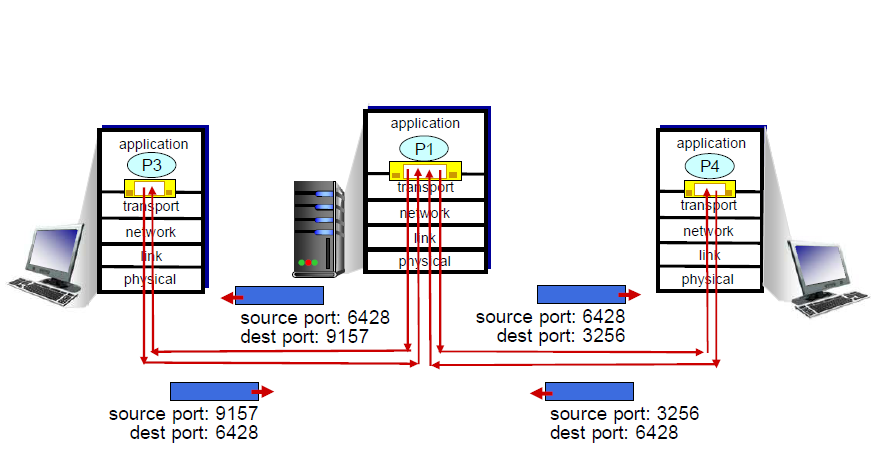
\includegraphics[width=0.75\linewidth]{./images/demultiplexing.png}
	\caption{Esempio di demultiplexing connectionless}
\end{figure}
\begin{figure}[htp]
	\centering
	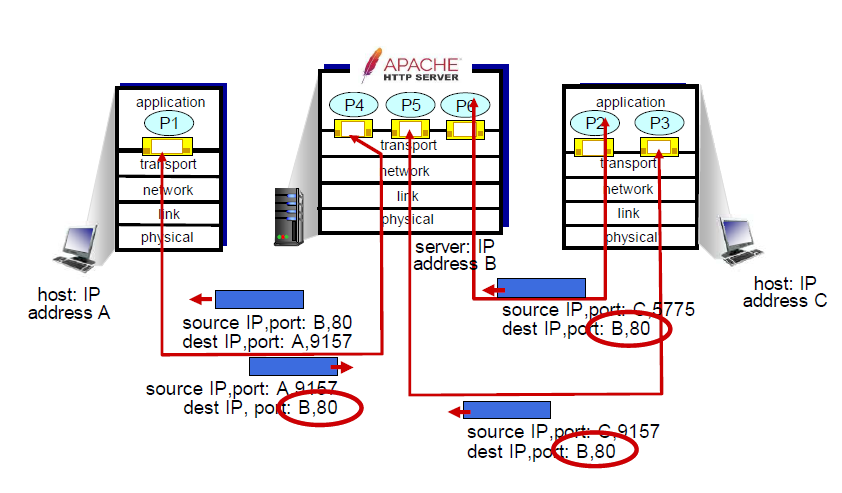
\includegraphics[width=0.75\linewidth]{./images/demultiplexingconnection.png}
	\caption{Esempio di demultiplexing connection-oriented}
\end{figure}

\newpage

\section{UDP - User Datagram Protocol}
TCP e UDP sono indubbiamente i \textbf{protocolli di trasporto dati} più popolari. Se il TCP è noto per la sua affidabilità (tramite i meccanismi di ACK da esso implementati), lo stesso non si può dire di UDP. Nonostante ciò, le funzionalità ridotte di UDP garantiscono un protocollo \textit{bare bones}, ridotto all'osso, \textbf{molto più veloce} e con meno \textit{overhead}.

\subsection{Caratteristiche di UDP}

\begin{itemize}
	\item È un protocollo di trasporto \textbf{bare-bones}, leggero, ma unreliable.\\ 
	Nessun handshake avviene tra il mittente e il destinatario. Ogni segmento UDP è gestito in maniera indipendente dagli altri, e non esistono vere e proprie "sessioni UDP". Per questo, è definito come un protocollo \textbf{connectionless}.
	
	\item L'header del protocollo UDP occupa 8 byte. 2 byte per la porta del mittente, 2 per la porta del destinatario, 2 per la lunghezza del messaggio (header UDP + dati) e 2 per il checksum. L'header  del protocollo TCP occupa dai 20 ai 60 byte: ben di più rispetto a UDP!
	
	\item È usato da applicazioni di streaming multimediale, comunicazione VoiP e DNS.  Si presta ad applicazioni che riescono a lavorare anche con \textbf{perdite di pacchetti}.
\end{itemize}

\subsection{Checksum (per UDP, ma anche TCP)}
È un meccanismo che consente di \textbf{rilevare errori di trasmissione}. Questi errori spesso consistono in \textbf{bit-flip}, che possono stravolgere del tutto i l significato dei dati trasmessi. Detto ciò, la verifica consiste nel calcolo di un \textbf{checksum}, in italiano \textbf{somma di controllo}, sia al mittente (che la inserirà nel frame) che al destinatario. La somma è calcolata in virtù dei dati contenuti nel frame. Se le due somme non dovessero coincidere, il pacchetto sarà da considerarsi fallato, e verrà scartato. 

\newpage

\section{Reliable Data Transfer - Trasferimento affidabile}
Data una rete di dispositivi comunicanti, quello che spesso si potrebbe pensare, è che la comunicazione sia sempre, a priori, affidabile. - \textit{Ogni pacchetto inviato arriva al mittente!} - E invece no. \textbf{Il canale di comunicazione è da considerarsi inaffidabile}, per una serie di motivi legati alla natura fisica del canale, ma anche a causa della "consapevolezza" limitata degli host: due host non conoscono reciprocamente i loro stati, se non comunicando. E se dei pacchetti si perdono? Nonostante ciò, tramite software, è possibile garantire un \textbf{trasporto affidabile} che rende più \textbf{robusta} la comunicazione. \textit{Creare un canale di comunicazione affidabile partendo da un canale fisico inaffidabile} è l'obiettivo posto dal topic \textbf{Reliable Data Transfer}.


\subsection{RDT - Introduzione}
Reliable Data Transfer è un meccanismo, descritto tramite \textbf{macchine a stati finiti}, che offre, nelle sue versioni, delle soluzioni software (per sender e receiver) per creare da canali fisici inaffidabili, connessioni affidabili. I meccanismi descritti da RDT, sono gli stessi seguiti da alcuni dei protocolli del livello di trasporto (banalmente, TCP).
\begin{figure}[htp]
	\centering
	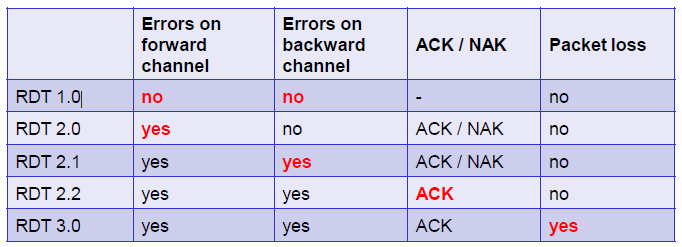
\includegraphics[width=0.5\linewidth]{./images/rdtversions.png}
	\caption{Versioni di RDT}
\end{figure}

Osserviamo in breve le caratteristiche dei vari RDT prima di studiarne le FSM al dettaglio:
\begin{itemize}
	\item 1.0. Non include nessun meccanismo effettivo, ma fa da base per le versioni successive.
	\item 2.0. Gestisce i pacchetti corrotti tramite segnali di ACK/NAK, ma non gestisce ACK e NAK corrotti.
	\item 2.1. Gestisce gli errori sul backward channel\footnote{Il backward channel è canale per l'invio dei segnali di ACK/NAK durante una connessione.}.
	\item 2.2. Si elimina il simbolo dedicato NAK, utilizzando in maniera differente gli ACK.
	\item 3.0. Tutte le precedenti versioni gestiscono solo pacchetti corrotti. Con questa versione, si verifica anche la perdita dei pacchetti, introducendo il meccanismo di time-out.
\end{itemize}


\subsection{RDT 1.0 - Canale perfetto, zero errori, zero perdite}
Presuppone un \textbf{canale perfetto} senza errori di bit e perdita di pacchetti. Sarà la base per le successive versioni di RDT.
Gli automi rimangono in attesa di un certo evento. La verifica dell'evento avviene tramite il cosiddetto "polling" o interrogazione.\\
Il \textbf{polling rate} stabilisce ogni quanto interrogare la condizione. Il polling rate DEVE essere stabilito, in quanto, altrimenti la verifica avverrebbe un numero di volte pari alla frequenza della CPU,  e si avrebbero comportamenti anomali.
\begin{figure}[htp]
	\centering
	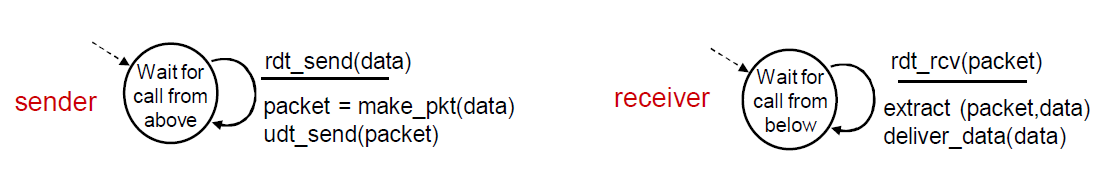
\includegraphics[width=1\linewidth]{./images/fsmrdt1.png}
\end{figure}
La FSM del sender si attiva quando riceve una richiesta per mandare dei dati. Quella del receiver, quando riceve dei pacchetti. \verb|deliver_data(data)| si riferisce a socket. 

\newpage

\subsection{RDT 2.0 - Canale imperfetto, errori sul forward}
Introduce \textbf{un checksum} e un \textbf{meccanismo di ACK} (senza checksum). Il sender manda un pacchetto e aspetta un feedback. \\ Si ipotizza che non si perdano pacchetti e che il backward sia perfetto. 

\begin{figure}[htp]
	\centering
	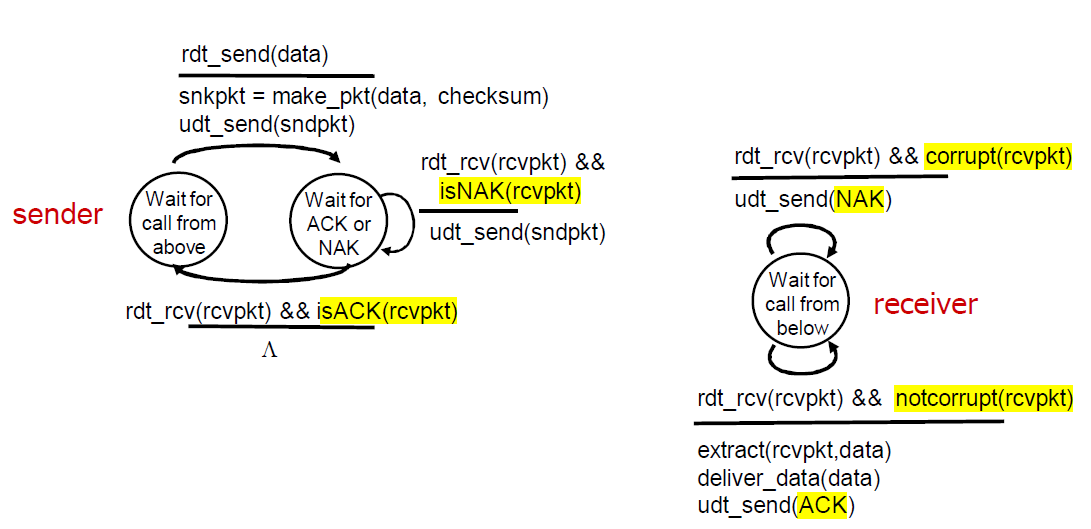
\includegraphics[width=1\linewidth]{./images/fsmrdt2.png}
\end{figure}


\begin{itemize}
	\item Il sender che ha appena mandato il pacchetto attende un ACK o un NAK.
	\item Il receiver verifica se il pacchetto è corrotto o meno, e in caso, manda un NAK o un ACK.
	\item Se il sender riceve ACK, ritorna allo stato iniziale ($\Lambda$), altrimenti rimanda il pacchetto arrivato corrotto.
\end{itemize}

Ipotizzare che il backward sia perfetto, è che ACK e NAK arrivino sempre integri, è azzardato: un ACK potrebbe corrompersi, diventare un NAK o non arrivare mai. Un hacker potrebbe sfruttare questa debolezza sostituendo tutti i pacchetti ACK con un NAK o un pacchetto differente, secondo l'approccio \textbf{Man-In-The-Middle}.

\newpage
\subsection{RDT 2.1 - Errori sul forward e sul backward}
L'RDT 2.1 nasce dall'esigenza di gestire un backward channel imperfetto, integrando un \textbf{checksum sugli ACK/NAK}. A ogni pacchetto viene annesso un \textbf{bit sequenza}, per disambiguare i pacchetti e gli ACK. A ogni pacchetto mandato, il sender integra un bit che si alterna tra 0 e 1. Quando il sender riceve un ACK/NAK corrotto, rimanda il pacchetto. Se il receiver riceve due volte lo stesso pacchetto con lo stesso bit sequenza, sa di dover \textbf{rimandare l'ACK}.

\subsubsection{Sender}
\begin{figure}[htp]
	\centering
	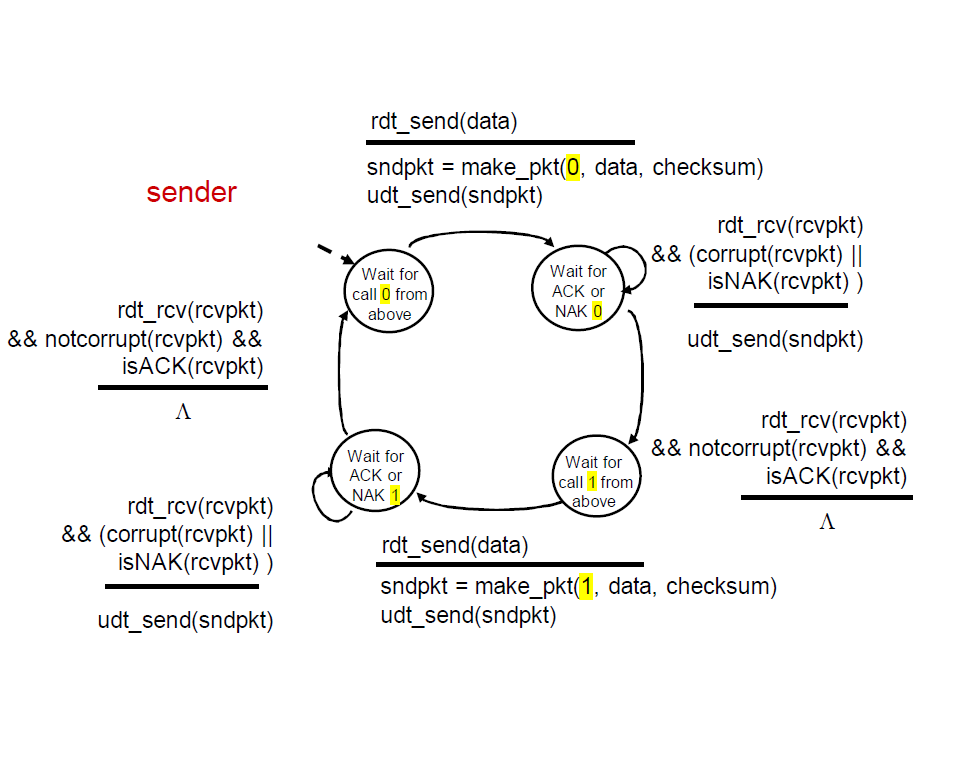
\includegraphics[width=0.8\linewidth]{./images/fsmrdt2.2sender.png}
\end{figure}

\subsubsection{Receiver}
\begin{figure}[htp]
	\centering
	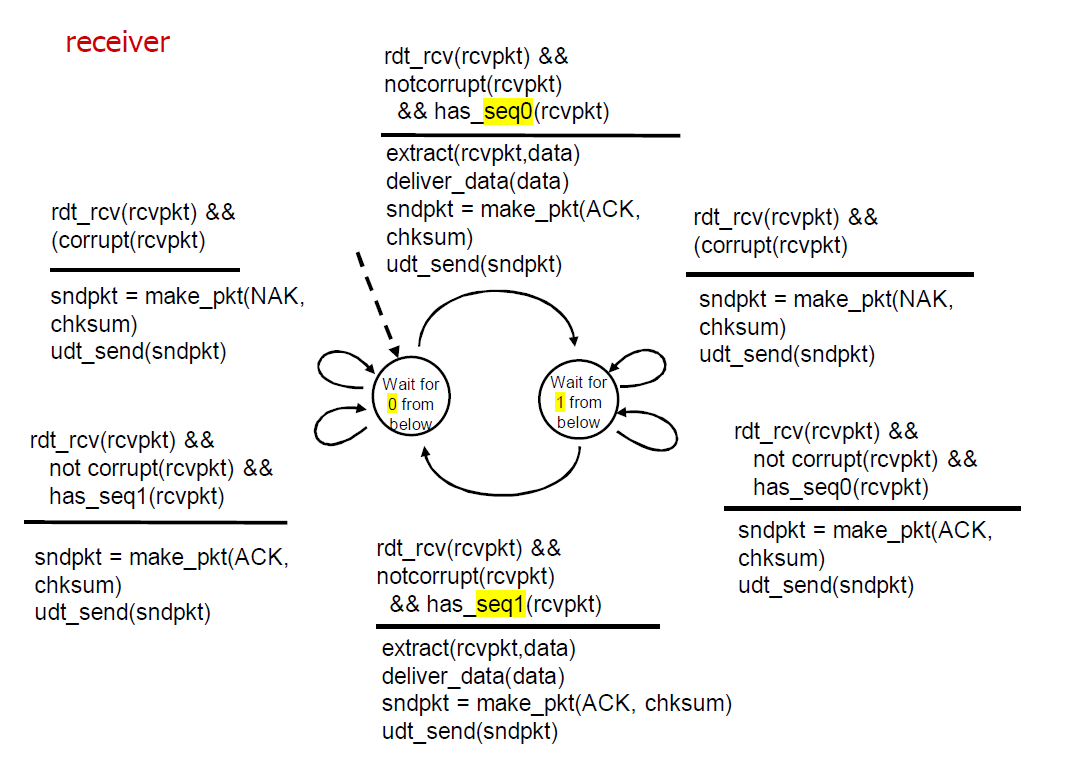
\includegraphics[width=0.8\linewidth]{./images/fsmdrt2.2receiver.png}
\end{figure}

\newpage

\subsection{RDT 2.2 - Eliminiamo il NAK!}
Rimuove il segnale NAK, cambiando leggermente il funzionamento dell'ACK:
\begin{itemize}
	\item Se il \textbf{pacchetto è stato consegnato correttamente}, viene mandato il segnale di \\ACK \underline{relativo al pacchetto}.
	\item Se il pacchetto \textbf{non è stato consegnato correttamente}, viene mandato il segnale di ACK \underline{dell'ultimo pacchetto ricevuto correttamente}.
\end{itemize}

\begin{figure}[htp]
	\centering
	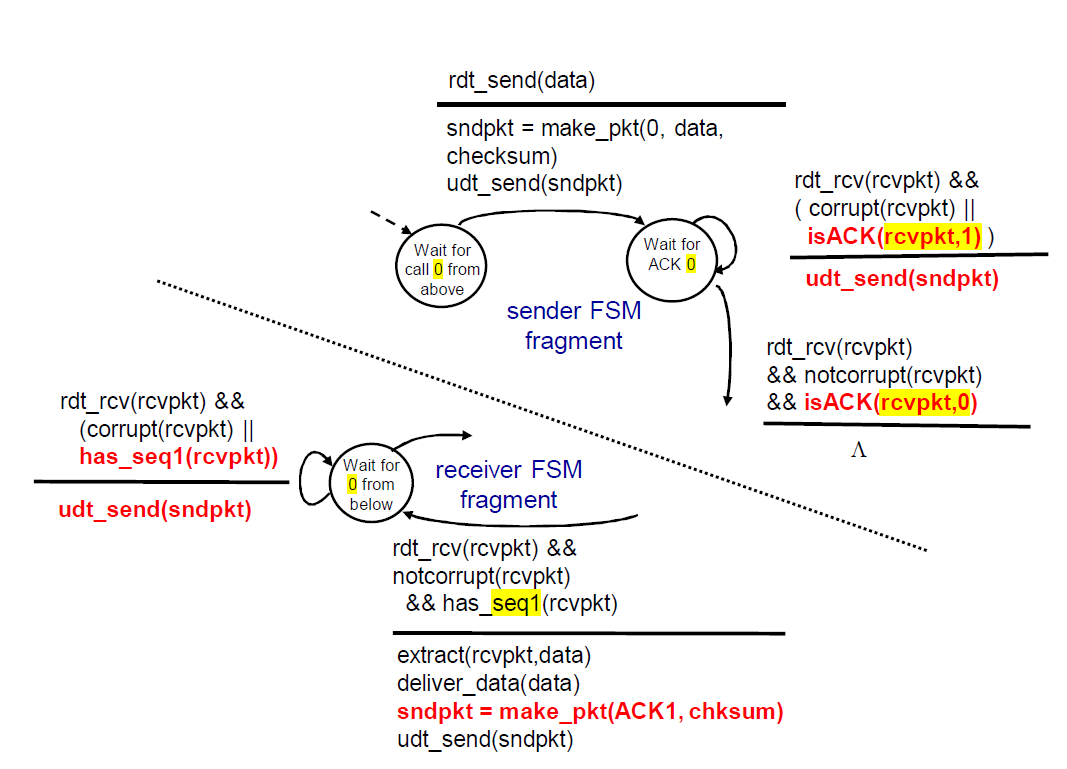
\includegraphics[width=1\linewidth]{./images/fsmdrt2.2.png}
\end{figure}
Nelle versioni precedenti, il NAK e l'ACK sono due segnali differenti. Un segnale che non è né ACK né NAK, a causa di una distorsione del segnale o un bit-flip, porta a dei segnali che il sistema non sa come gestire. \textbf{Rimuovere la classe dei segnali NAK ci permette di non cadere in} queste \textbf{ambiguità}.\\
Tuttavia, non contempliamo ancora la perdita di pacchetti.
\newpage

\subsection{RDT 3.0 - Errori e perdite}
Assumiamo (finalmente) che il canale possa perdere pacchetti (sia dati, che ACKs).\\ Gestiamo il tutto con la \textbf{temporizzazione}.

\subsubsection{Sender}
\begin{figure}[htp]
	\centering
	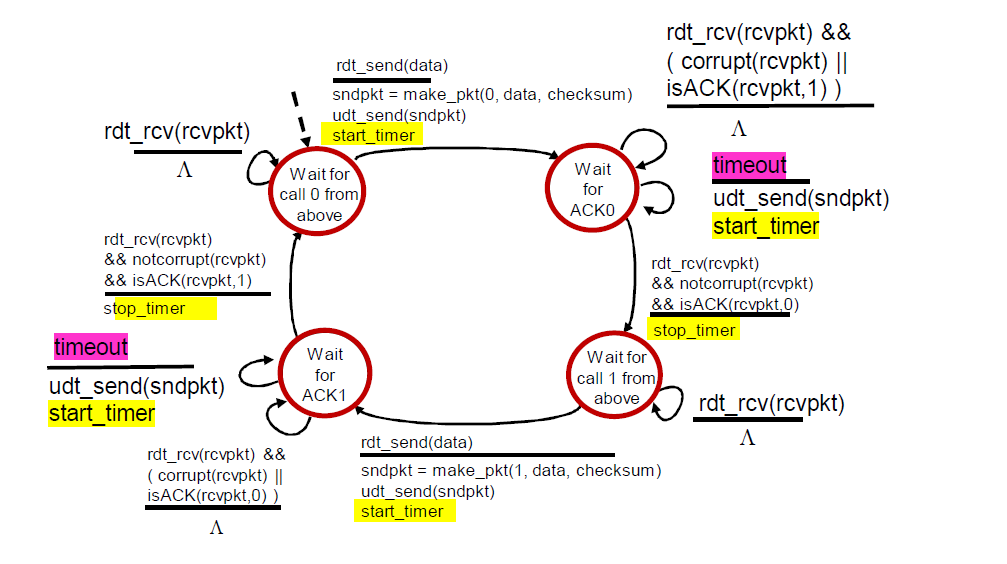
\includegraphics[width=1\linewidth]{./images/fsmrdtsender.png}
\end{figure}

\subsubsection{Receiver}
Macchina a stati finiti analoga a quella di RDT 2.2. La temporizzazione è gestita esclusivamente al sender.

\newpage

\section{Calcolo del Throughput}
Il \textbf{throughput} è un'indice della capacità di trasmissione di un canale di comunicazione. 

$$
\text{Throughput} = \frac{\text{Numero di bit (o byte) trasmessi con successo}}{\text{Tempo impiegato}}
$$

\subsection{Throughput teorico}
Consideriamo un canale con \textbf{Bandwidth} $BW = 10 \text{ Mbps}$ (Megabit per secondo).
Questo vuol dire in un secondo possono essere trasmessi $10^7$ bit. Un bit viene 
trasmesso in $\frac{1}{10^7} = 0.1 \mu s$ (microsecondo).

\subsubsection{Tempo di trasmissione di un frame}
Consideriamo ora di voler trasmettere un frame di 1500 byte, ovvero $1500 \cdot 8 = 12000$ bit.\\
Per trasmettere un frame, impieghiamo il seguente tempo:
$$
T_\text{frame} = \frac{\text{Dimensione del frame (in bit)}}{\text{Bandwidth (in bit/s)}} = \frac{12000 \ bit}{10^7 \ bit/s} = 0.0012s  = 1200 \mu s  
$$

\subsubsection{Tempo di propagazione}
Nella trasmissione dobbiamo anche considerare il tempo di propagazione, che è il tempo richiesto al segnale per arrivare fisicamente da host $A$ a $B$: supponiamo che lo spazio di trasmissione sia pari ad $1km$. 
Supponiamo che la velocità di trasmissione, che dipende dal mezzo che usiamo e dalle sue condizioni, sia  $v \approx 200.000km/s$, e che sia un valore costante.
Il tempo di propagazione è dato dal rapporto spazio/velocità.

$$
T_\text{propagazione} = \frac{\text{Spazio di trasmissione}}{\text{Velocità di trasmissione}} = \frac{1km}{200000 km/s} = \frac{1}{200000} s = 5\cdot 10^{-6} s =  5 \mu s
$$

Con questa informazione possiamo anche andare a calcolare il numero di bit che possono occupare il canale contemporaneamente, ovvero
$$
\text{Bandwidth (in bit/s)}\cdot T_\text{propagazione}\text{(in s)} = 10^7\text{ bit/s} \cdot 5 \cdot 10^{-6}\text{ s} = 50 \text{ bit}
$$

\subsubsection{Tempo di trasferimento}
Ora abbiamo tutte le informazioni necessarie per calcolare il tempo di trasferimento complessivo.\\
Esso indica il tempo che il frame necessita per essere trasferito (ipotizzando che non ci siano da considerare variabili relative ai tempi di connessione, ACK, etc.).

$$
T_\text{trasferimento} = T_\text{frame} + T_\text{propagazione} = 1200 \mu s + 5 \mu s = 1205 \mu s
$$

\begin{figure}[htp]
	\centering
	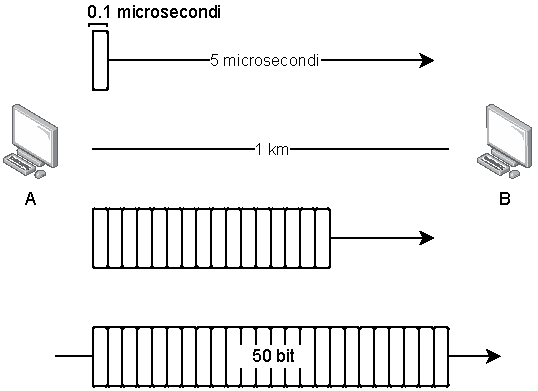
\includegraphics[width=0.65\linewidth]{./images/throughput.pdf}
\end{figure}

\newpage

\subsection{Throughput effettivo}
Quello appena calcolato, è da definirsi un \textbf{througput teorico}. Il \textbf{throughput effettivo} è influenzato anche da altri elementi di attesa, quali \textit{Round Trip Time}, tempi di elaborazione e di trasferimento relativi agli \textbf{ACK}.

\subsubsection{RTT - Round Trip Time}
Il Round Trip Time può essere stimato, e dedicheremo una sezione proprio alle metodologie di stima. È definito come il tempo che intercorre tra l'inizio dell'invio di un messaggio, e la ricezione della sua conferma.

\subsubsection{Tempo di trasmissione ACK}
Il segnale di ACK ha solitamente dimensione pari a $64 \ byte = 64 \cdot 8 \ bit = 512 \ bit$. Ne consegue che:
$$
T_{ACK} = \frac{\text{Dimensione dell'ACK (in bit)}}{\text{Bandwidth (in bit/s)}} = \frac{512}{10^7} = 0.0000512 s = 51.2  \mu s 
$$

\subsubsection{Tempo di trasferimento effettivo}

Stimiamo un tempo di elaborazione dell'ACK di $3 \mu s$ e un RTT di $10 \mu s$ ($5\mu s \cdot 2$, ovvero il $T_{propagazione}$, ma in andata e ritorno).
Otteniamo quindi un tempo complessivo pari a:

$$
T_\text{effettivo} = T_{frame} + T_{ACK} + RTT + \text{Elaborazione ACK} = 1200 + 51.2 + 10  + 3 =  1264.2 \mu s
$$

\subsubsection{Calcolo del Throughput effettivo}
Calcoliamo ora il throughput effettivo, mettendo a rapporto il numero di bit per frame da trasmettere con il tempo di trasferimento totale

$$
\frac{\text{Dimensione del frame (in bit)}}{\text{Tempo totale di trasmissione (in s)}} = \frac{12000}{1264.2 \cdot 10^{-6}} = 9.492 \text{ Mbps}
$$

Osserviamo con piacere che otteniamo un valore molto simile alla larghezza di banda. I fattori esterni non hanno creato particolari \textbf{colli di bottiglia} alla nostra capacità di trasmissione! Il mezzo è ben sfruttato.

\subsubsection{Conclusioni sul throughput reale}
Il throughput reale è fortemente influenzato dal tempo di elaborazione dei segnali di ACK e dall'RTT. Nel caso appena studiato, la \textbf{bandwidth è ben sfruttata}, ma quando l'RTT sarà dell'ordine dei millisecondi\footnote{Recap sui prefissi: milli- = $10^{-3}$, micro- = $10^{-6}$, nano- = $10^{-9}$, kilo- = $10^{3}$, mega- = $10^{6}$, giga- = $10^{9}$;}, e non dei microsecondi, otterremo dei cali di performance non da poco. 




\subsection{Considerazioni}
Il \textbf{tempo di propagazione} è il tempo richiesto ad un segnale per trasmettersi da un punto all'altro. Precedentemente, abbiamo stimato l'$RTT$ come due volte il $T_{propagazione}$. Nel protocollo TCP è presente il meccanismo di Three Way Handshake: questo implica ulteriore ritardo per l'RTT, che può di gran lunga superare la stima calcolata. Se i valori sono diversi, nel calcolo, andremo a considerare il maggiore tra i due.\\
Inoltre, se la bandwidth effettiva calcolata è superiore a quella teorica, allora la bandwidth teorica funge da collo di bottiglia: la bandwidth effettiva sarà uguale a quella teorica, in quanto limite massimo.

\subsection{Ping}
Il comando \verb|ping| è un utility che permette di calcolare l'RTT necessario per la connessione ad un server, e fornisce anche la percentuale di pacchetti persi. Usa il protocollo ICMP.

\newpage


\section{Modalità Pipeline}
È una modalità che consente di aumentare il throughput di una rete. Invece di inviare un singolo frame e aspettare il rispettivo ACK (modalità esposta in precedenza, nota come modalità \textbf{stop-and-wait}), si stabilisce una window di $n$ frame di cui si \textbf{potranno aspettare gli ACK contemporaneamente}. Questo\textbf{ riduce di molto l'influenza del $RTT$ sul throghput}, riducendo di molto l'\textit{overhead} delle singole trasmissioni. L'utilizzo della modalità pipeline è chiaramente più \textbf{vantaggiosa della stop-n-wait}, soprattutto nel contesto di \textbf{reti ad alta latenza}. La finestra d'invio verrà succesivamente indicata con il nome \verb|cwnd|, nel contesto del controllo della congestione.

\subsubsection{Esempio}
Vogliamo mandare pacchetti di 1000 byte.\\
$BW = 1 Gbps = 1000 \ Mbps = 1\cdot10^{9} \ bps$.\\
$RTT=30 \ ms$.\\
Il tempo teoricamente richiesto sarebbe

$$
T_{frame} = \frac{\text{Dimensione dati (in bit)}}{\text{Bandwidth (in bit/s)}} = \frac{8\cdot 10^3 \text{ bit}}{1\cdot10^9 \text{ bit/s}}= 8\cdot 10^{-6} \ s = 8 \mu s
$$
a cui aggiungere $30000 \mu s$. Otteniamo un througput effettivo di
$$
\frac{\text{Dimensione del frame (in bit)}}{\text{Tempo totale di trasmissione (in s)}} = \frac{8000 \text{ bit}}{30008 \mu s} = \frac{8000 \text{ bit}}{30,008 \ ms} = \frac{8000 \text{ bit}}{0,030008 \ s} = 266595 \ bps \approx 267 \ Kbps
$$

Creando un grande collo di bottiglia alla nostra bandwidth di $1 \ Gbps$. Tuttavia, il canale potrebbe ospitare contemporanemente un numero di bit pari a 
$$
\text{Bandwidth} \cdot RTT = 1\cdot 10^9 \cdot 3\cdot 10^{-2} = 3 \cdot 10 ^7 \, \text{bit}
$$

Tuttavia, se decidiamo di sfruttare la modalità pipeline, potremmo pensare di mandare più frame contemporaneamente. Il canale, infatti, supporterebbe al più:

$$
\frac{30\,000\,000 \, \text{bit}}{8\cdot 10^3 \ \text{bit/frame}} = 3750 \, \text{frame}
$$

Stabilendo una finestra di $n$ frame, con un valore di $n$ opportuno, sarà possibile sfruttare al meglio la bandwidth del canale! Idealmente, in questo caso, $n=3750$.

\subsection{Contro della modalità pipeline}
Questa modalità richiede una gestione più complessa della ricezione degli ACK: 
\begin{itemize}
	\item Bisogna gestire in maniera opportuna invio e ricezione e grandezza della finestra di frame.
	\item Diventa obbligatorio usare più di un bit per il numero di sequenza, in modo proporzionale alla dimensione della finestra.
\end{itemize}

\newpage


\subsection{Algoritmi per la pipeline - Go-Back-n}
Usa un approccio \textbf{sliding windows} per gestire la pipeline.
Il server stabilisce una window di $n$ frame.
\subsubsection{Sender}
\begin{figure}[htp]
	\centering
	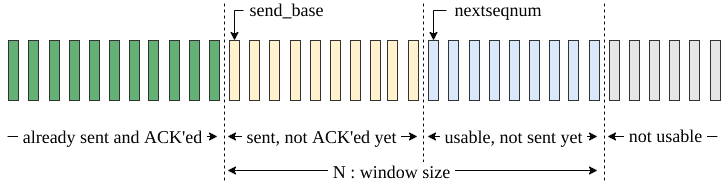
\includegraphics[width=1\linewidth]{./images/gobackn.png}
\end{figure}
Ogni volta che il primo frame della finestra viene mandato, questa "scorre" di un frame verso quelli ancora da mandare. Individuiamo quattro insiemi disgiunti di frame:
\begin{itemize}
	\item I frame mandati non confermati (ACKed, prima parte della finestra).
	\item I frame non mandati ma utilizzabili (seconda parte della finestra).
	\item Prima della finestra, abbiamo i frame mandati e confermati.
	\item Dopo la finestra, i frame non utilizzabili.
\end{itemize}

\subsubsection{Receiver}
Riceve i pacchetti e risponde con gli \verb|ACK| rispettivi. Quando non riceve il pacchetto giusto\footnote{Un esempio di pacchetto non corretto? Il pacchetto con numero di sequenza 3 dopo aver ricevuto il pacchetto 1 è sbagliato: manca il pacchetto 2.}, scarta il pacchetto, manda un duplicato dell'ultimo \verb|ACK| ricevuto correttamente.

\begin{figure}[htp]
	\centering
	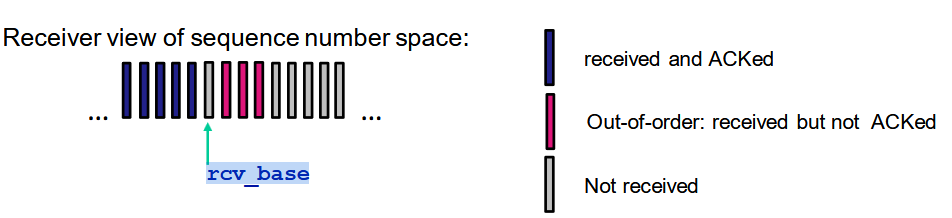
\includegraphics[width=1\linewidth]{./images/gobackn2.png}
\end{figure}


\subsubsection{Criticità del Go-Back-N}
Osserviamo che se l'$n$-esimo pacchetto non è stato ricevuto con successo, tutti i successivi pacchetti mandati verranno scartati. Nell'immagine della prossima pagina, si evidenzia come il primo inoltro dei pacchetti 3, 4 e 5 sia praticamente cestinato. È un algoritmo solido e reliable, ma rischia grosse perdite di tempo a causa dell'\verb|ACK| cumulativo.
\newpage

\begin{figure}[htp]
	\centering
	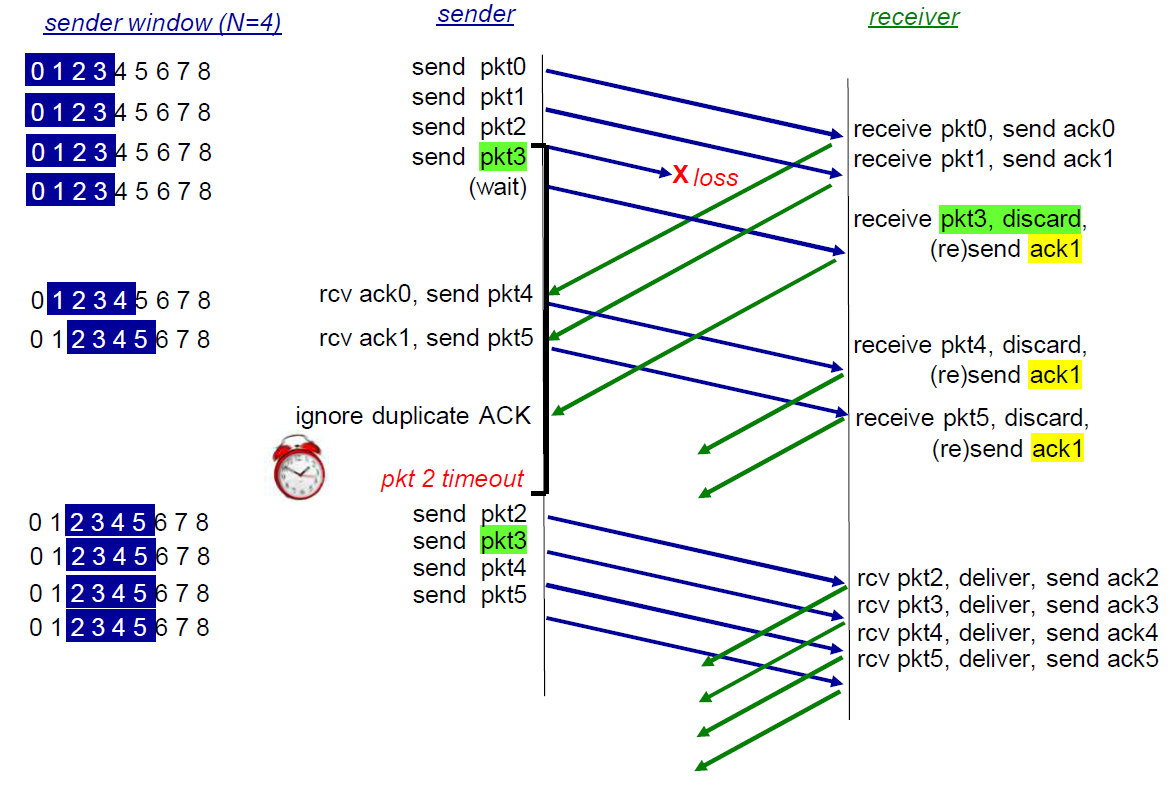
\includegraphics[width=1\linewidth]{./images/gobacknn.png}
	\caption{Go-back-n.}
\end{figure}

\newpage

\subsection{Algoritmi per la pipeline - Selective Repeat}
Col selective repeat, i frame che si perderebbero durante il time-out, sono bufferizzati in una memoria all'interno del dispositivo (in una look-up-table), in modo da velocizzarne il caricamento e non dover richiede il reinvio dal sender. Gli ACK dei pacchetti ricevuti correttamente vengono rimandati regolarmente. 

\begin{figure}[htp]
	\centering
	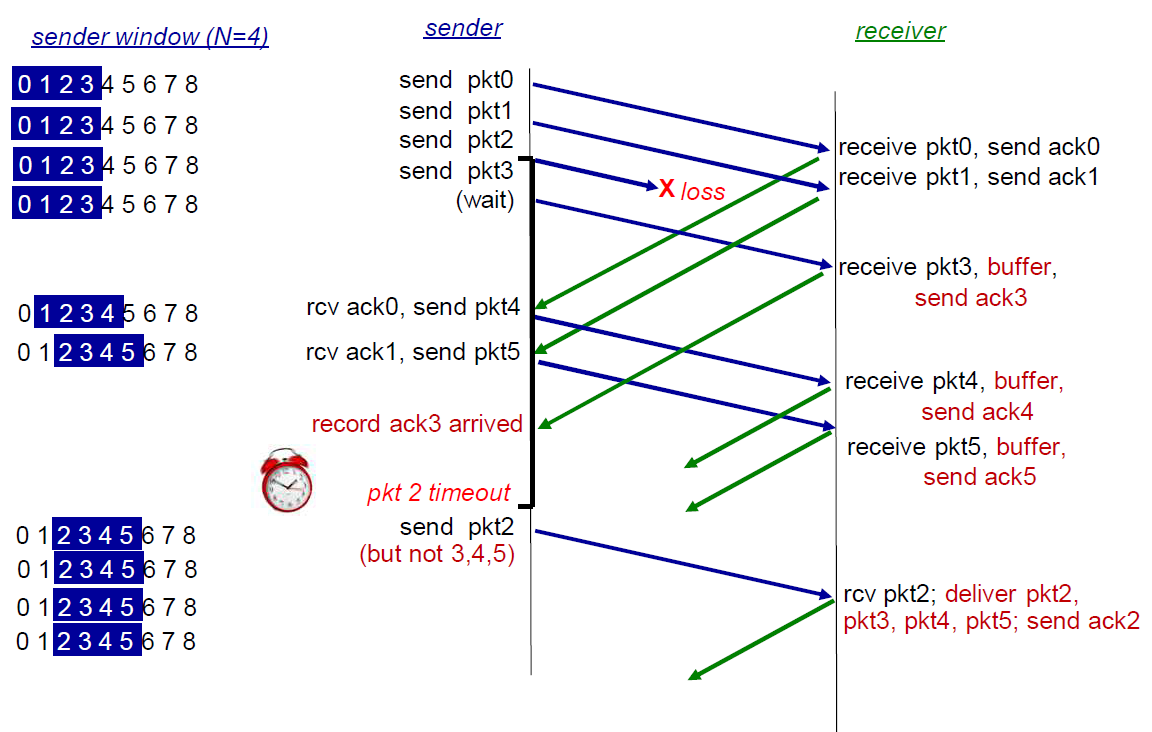
\includegraphics[width=0.75\linewidth]{./images/selectiverepeat.png}
\end{figure}

\subsubsection{Sender}
\begin{itemize}
	\item Trasmette fino a $n$ pacchetti \textbf{senza attendere ACK}.
	\item Ogni pacchetto ha un \textbf{timer personale} per la ritrasmissione.
	\item Ricevuto l'ACK dell'$n$-esimo pacchetto, viene \textbf{marcato come ricevuto}.
	\item Il primo frame della windows è sempre il primo frame della sequenza non ancora confermato.
\end{itemize}
\subsubsection{Receiver}
\begin{itemize}
	\item \textbf{I pacchetti non ricevuti in ordine vengono inseriti in un buffer}.
	\item A ogni pacchetto ricevuto, consegue l'invio di un \textbf{ACK}.
	\item Se l'$n$-esimo pacchetto viene ricevuto, e ci sono \textbf{pacchetti subito successivi bufferizzati}, questi vengono \textbf{passati al layer superiore}.
	\item Il receiver potrebbe ricevere un pacchetto con \textbf{numero di sequenza precedente alla finestra}: in tal caso, \textbf{reinvierà l'ACK}.
\end{itemize}

\subsubsection{Pro del Selective Repeat}
\textbf{Meno ritrasmissioni inutili}, maggiore efficienza in canali con alta perdita di pacchetti.
\subsubsection{Contro del Selective Repeat}
\begin{itemize}
	\item Il buffer non ha \textbf{memoria infinita}, potrebbe saturarsi.
	
	\item Possono esserci \textbf{ambiguità} causati dai \textbf{codici sequenza ripetuti}. Per non incorrere in questi problemi, deve essere rispettata la seguente disequazione:
	$$
	\text{K-seq (Numero max sequenza)} \geq 2 \cdot \text{Window Size}
	$$
	
	\begin{figure}[htp]
		\centering
		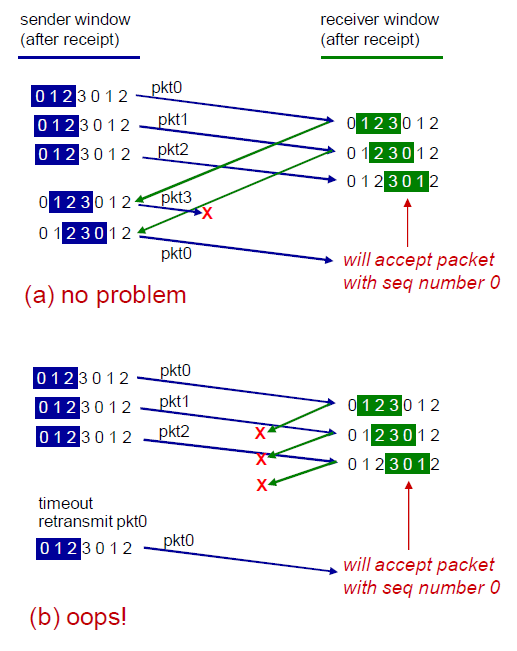
\includegraphics[width=0.75\linewidth]{./images/selectiverepeat3.png}
		\caption{Ambiguità dei codici sequenza nel Selective Repeat}
	\end{figure}
\end{itemize}

\newpage

\section{TCP}
Sta per \textbf{Transmission Control Protocol}. Assieme a UDP, è il \textbf{protocollo del layer di trasporto più importante}. Sfruttato da tantissime applicazioni del layer superiore, offre un trasporto affidabile, basato sui meccanismi della modello RDT 3.0.  Tra le sue funzionalità, offre:

\begin{itemize}
	\item \textbf{Addressing} / \textbf{multiplexing}.
	\item Stabilimento, gestione e terminazione della \textbf{connessione}.
	\item \textbf{Data Handling} e impacchettamento.
	\item \textbf{Trasferimento dei dati} (banalmente).
	\item Fornisce \textbf{specifiche} relative alla reliability della rete.
	\item \textbf{Controllo del flusso} e gestione della \textbf{congestione}.
\end{itemize}

\subsubsection{Cosa non fornisce il TCP?}
\begin{itemize}
	\item Non garantisce \textbf{sicurezza}.\\
	È \textbf{vulnerabile} ad hacking, attacchi man-in-the-middle, sniffing e simili.
	\item Non da \textbf{specifiche sull'application layer}.\\
	Non fa ipotesi sui layer superiori (ed è giusto che sia così! Altrimenti le applicazioni si dovrebbero adattare alle ipotesi fatte da TCP).
	\item Non mantiene i \textbf{message boundaries}.\\
	Non stabilisce i confini dei messaggi. Sono i protocolli del layer applicativo che stabiliscono come interpretare i messaggi e ricostruire i dati, tramite caratteri di terminazione, lunghezze prestabilite o header.
	
	\item Non da \textbf{garanzie sul throughput}.
	
	\item \textbf{Non supporta trasferimento multicast}, ossia trasferimento da un mittente a molti destinatari in una sola operazione.
\end{itemize}

\newpage

\subsection{TCP-State Model}
È un diagramma degli stati che descrive le fasi di una connessione TCP.
\begin{figure}[htp]
	\centering
	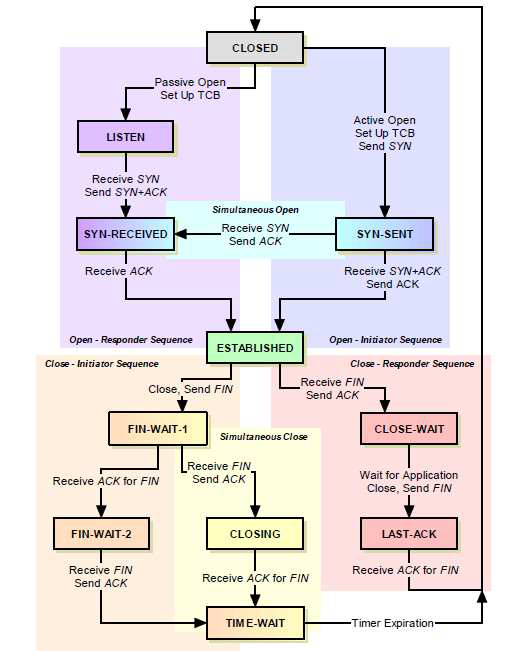
\includegraphics[width=0.7\linewidth]{./images/TCPSTATEMACHINE.png}
\end{figure}
\subsection{Fasi di apertura della connessione (3-way-handshake)}
\begin{enumerate}
	\item CLOSED.
	\begin{enumerate}
		\item Stato iniziale, nessuna connessione attiva.
		\item Un'applicazione può avviare una connessione o attenderne una in ingresso.
	\end{enumerate}
	\item LISTEN (solo lato server).
	\begin{enumerate}
		\item Il server è in ascolto, pronto a ricevere connessioni (passive open).
		\item Se riceve un segmento \verb|SYN|, risponde con \verb|SYN-ACK| e passa allo stato \verb|SYN|
	\end{enumerate}
	\item SYN-SENT (solo lato client).
	\begin{enumerate}
		\item Il client avvia una connessione inviando un segmento \verb|SYN|
		\item Se riceve \verb|SYN+ACK| risponde con \verb|ACK| e la connessione è stabilita (passando a \verb|ESTABLISHED|)
	\end{enumerate}
	\item SYN-RECEIVED
	\begin{enumerate}
		\item Il server ha ricevuto \verb|SYN| e inviato il \verb|SYN-ACK|
		\item Quando riceve l'\verb|ACK| finale dal client, la connessione è stabilita (\verb|ESTABLISHED|).
	\end{enumerate}
	\item ESTABLISHED
	\begin{enumerate}
		\item Stato operativo della connessione in cui i dati vengono trasmessi tra client e server.
		\item La connessione si trova in questo stato finché non viene chiusa.
	\end{enumerate}
	\subsection{Fasi della chiusura della connessione (4-way-handshake)}
	\item FIN-WAIT-1.
	\begin{enumerate}
		\item Il lato che inizia la chiusura invia un segmento \verb|FIN|.
		\item Attende un \verb|ACK| per il \verb|FIN| o un \verb|FIN| dall'altro lato.
	\end{enumerate}
	\item CLOSE-WAIT.
	\begin{enumerate}
		\item Il lato che riceve il \verb|FIN| invia un \verb|ACK| e passa in \verb|CLOSE-WAIT|.
		\item Aspetta che l'applicazione chiuda il socket, poi invia un \verb|FIN|.
	\end{enumerate}
	\item FIN-WAIT-2
	\begin{enumerate}
		\item Il lato che ha inviato il primo \verb|FIN| ha ricevuto un \verb|ACK| ed è in attesa del \verb|FIN| dell'altro lato
	\end{enumerate}
	
	\item LAST-ACK.
	\begin{enumerate}
		\item Il lato che ha ricevuto il \verb|FIN| deve terminare, invia un \verb|FIN| e attende un \verb|ACK|.
	\end{enumerate}
	
	\item TIME-WAIT
	\begin{enumerate}
		\item Dopo aver ricevuto l'ultimo \verb|ACK|, il lato iniziatore della chiusura entra in \verb|TIME-WAIT| per un certo tempo (solitamente il doppio del Maximum Segment Timeline).\\
		Questo assicura che l'altro lato abbia ricevuto l'ACK finale prima di tornare a \verb|CLOSED|.
	\end{enumerate}
	
	\item CLOSING
	\begin{enumerate}
		\item Caso raro in cui entrambi i lati inviano un \verb|FIN| contemporaneamente.
		\item Entrambi inviano e ricevono un \verb|ACK|, poi passano a \verb|TIME-WAIT|.
	\end{enumerate}
\end{enumerate}
\newpage

\subsection{Struttura dei segmenti del TCP}
Gli header dei segmenti TCP occupano \textbf{dai 20 ai 60 byte}, (ricordiamo che gli header UDP occupano solo 8 byte). 

\begin{figure}[htp]
	\centering
	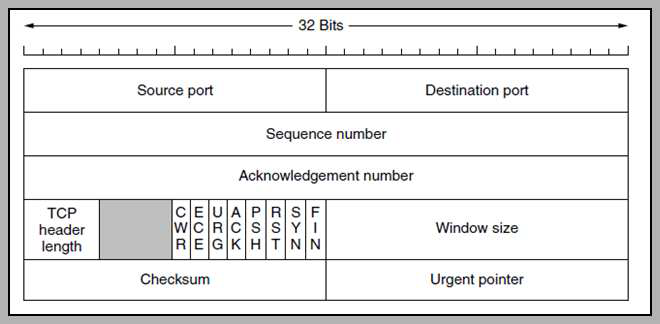
\includegraphics[width=0.8\linewidth]{./images/SEGMENTCP.png}
\end{figure}

\begin{itemize}
	\item \textbf{Source port} e \textbf{Destination port} indicano le porte dei processi del sender e receiver associati alla connessione TCP.  16 bit ciascuno.
	
	\item \textbf{Sequence number}. \\
	Viene incrementato di $n$ ogni volta che $n$ byte sono trasmessi. Mandato un pacchetto TCP di \\1400 byte, il prossimo valore sarà il precedente numero di sequenza + 1400. 32 bit.
	
	\item \textbf{Acknowledgment number}.\\
	Se \verb|ACK| è abilitato, ritorna il sequence number del prossimo pacchetto che si aspetta di ricevere. \\
	32 bit.
	
	\begin{Verbatim}
		CLIENT                  SERVER
		#seq = 1
		Len = 669     -->
		<--       ACK (669 + 1 =) 670
		#seq = 670
		Len = 1460    -->
		<--       ACK (670 + 1460 =) 2130
		#seq = 2130
		Len = 1460    -->
		<--       ACK 3590
		[...] 
		END OF TCP CONNECTION
	\end{Verbatim}
	
	
	Notiamo che \textbf{il protocollo TCP è full-duplex}: gli host ricevono e mandano dati nella stessa connessione.
	
	\item \textbf{TCP header length} o \textbf{Data Offset}.\\
	Specifica il numero di double word (4 byte) dell'header del segmento TCP. 4 bit. 
	\item Dello spazio libero per sviluppi futuri del protocollo. 4 bits.
	
	\item \textbf{8 flags}, un bit per flag.
	\begin{itemize}
		\item \verb|CWR| Congestion Window Reduced.\\ 
		A 1 indica che l'host sorgente ha ricevuto un segmento TCP con il flag ECE impostato a 1.
		\item \verb|ECE| Explicit Congestion Notification-Echo.\\ 
		A 1 indica che l'host supporta ECN durante il 3-way handshak
		\item \verb|URG|.\\
		A 1 indica che nel flusso sono presenti dati urgenti specificati nel campo urgent pointer.
		\item \verb|ACK|.\\
		A indica che il campo Acknowledgment number è valido.
		\item \verb|PSH|.\\
		A 1 indica che i dati in arrivo non devono essere bufferizzati ma passati subito ai livelli superiori dell'applicazione.
		\item \verb|RST|.\\
		A 1 indica che la connessione non è valida; viene utilizzato in caso di grave errore; a volte utilizzato insieme al flag ACK per la chiusura di una connessione.
		\item \verb|SYN|.\\
		A 1 indica che il mittente del segmento vuole aprire una connessione TCP con l'host destinatario e specifica nel campo Sequence number il valore dell'Initial Sequence Number (ISN); questo sincronizza i numeri di sequenza dei due host. L'host che ha inviato il SYN deve attendere dall'host remoto un pacchetto SYN/ACK.
		\item \verb|FIN|.\\
		A 1 indica che l'host mittente del segmento vuole chiudere la connessione TCP. Il mittente attende la conferma dal ricevente (con un FIN-ACK). La connessione sarà ancora chiusa per metà: l'host che ha inviato FIN non potrà più inviare dati, mentre l'altro host ha il canale di comunicazione ancora disponibile. L'altro host dovrà inviare il pacchetto con FIN impostato. Dopo il relativo FIN-ACK, la connessione sarà considerata completamente chiusa.
	\end{itemize}
	
	\item \textbf{Window size}.\\ 
	Indica la dimensione della finestra di ricezione del mittente. 16 bit.
	
	\item \textbf{Checksum}.\\
	Serve a verificare la validità del segmento. 16 bit.
	
	\item \textbf{Urgent pointer}.\\
	Punta a un dato urgente, ma solo se \verb|URG |=1. Indica l'offset in byte dal sequence number ai dati urgenti all'interno del flusso. 16 bit.
	
	\item Sotto troveremo anche dei byte dedicati ad ulteriore possibili \textbf{impostazioni}, e, chiaramente, lo spazio dedicato ai \textbf{dati da inviare}.
\end{itemize}


\newpage

\section{Migliorare il Througput - MMS e MTU}
I meccanismi appena esposti rendono TCP un protocollo affidabile. Tuttavia, anche il \textbf{throughput} è un fattore da tenere in considerazione. Per massimizzare il throughput, dobbiamo analizzare una serie di parametri.

\subsection{MMS, MTU}
\begin{itemize}
	\item \textbf{MMS - Maximum Segment Size}.\\
	Indica la dimensione massima dei dati che possono essere inviati in un singolo segmento TCP (esclusi gli header TCP/IP). Questo valore viene solitamente scelto in virtù dal frame più grande che il sender può trasmettere. 
	
	\item \textbf{MTU - Maximum Transmission Unit}.
	$$\text{MSS} + \text{dimensione dell'header TCP + dimensione dell'header IP}$$
	
\end{itemize}

Il protocollo TCP richiede un MTU minimo di 576 bytes, e quindi un MSS minimo di 536 bytes + 40 bytes di header IP (20 byte) e TCP (20 bytes).

\section{Migliorare il Througput - Retransmission Time-Out}
Affrontando l'argomento del \textbf{Reliable Data Transfer}, abbiamo spiegato che il meccanismo di \textbf{temporizzazione è fondamentale} per ottenere un trasferimento dati \textbf{reliable}. Nonostante ciò, bisogna trovare un buon \textbf{compromesso} per non impattare negativamente sul througput. \textbf{Il time-out va stabilito in funzione del Round Trip Time}.

\begin{itemize}
	\item \textbf{Time-out troppo lungo?}\\
	Reazione troppo lenta alla perdita dei pacchetti. Conseguenza di un time-out di molto maggiore dell'RTT.
	
	\item \textbf{Time-out troppo corto?}\\
	Gli ACK potrebbero non arrivare in tempo, richiedendo ritrasmissioni non necessarie. Time-out quanto o poco più lungo dell'RTT.
\end{itemize}

Per decidere il tempo opportuno per il time-out, bisogna avere una stima \footnote{Il round trip time è un valore misurabile, ma variabile. L'obiettivo che ci poniamo è stimare sempre il prossimo valore dell'RTT in funzione dei precedenti. Ricordiamo inoltre che ping permette di ottenere il Round Trip Time con un server.} valida dell'RTT. 


\subsection{Stimare il Round Trip Time}
Il Sample\_RTT è la misura del tempo di trasmissione di un segmento. La misura avviene dall'invio del segmento fino alla ricezione dell'ACK.\\
Un algoritmo che potrebbe essere utilizzato per stimare il time-out è quello di \textbf{Karn}: questo tuttavia, non tiene conto di possibili ritrasmissioni dei pacchetti non-acknowledged, che nella realtà avvengono molto spesso.\\
Utilizzeremo quindi una \textbf{media pesata} chiamata \textbf{Exponential Weighted Moving Average}.

\newpage

\subsection{Exponential Weighted Moving Average - EWMA}
Il peso, ovvero l'influenza dei campioni passati sulla media calcolata decresce in maniera esponenziale.

$$
\text{Estimated\_RTT}_n = (1-\alpha)\cdot \text{Estimated\_RTT}_{n-1} + \alpha \cdot  \text{Sample\_RTT}_n
$$

Dove il $\text{Sample\_RTT}_n$ è l'$n$-esima misurazione. Il valore $\alpha$ è detto \textbf{weighted value}, e stabilisce il peso dell'ultima misura rispetto a quello dell'ultima stima sulla media. Un valore tipico è $\alpha = \frac{1}{8} = 0,125$. Il valore di $\alpha$ varia, non è raro l'utilizzo di tecnica try and error per trovare il valore che permette di ottenere stime ottime.
Euristiche varie e tecnologie AI sono utilizzate per ottenere stime via via più accurate.

\begin{figure}[htp]
	\centering
	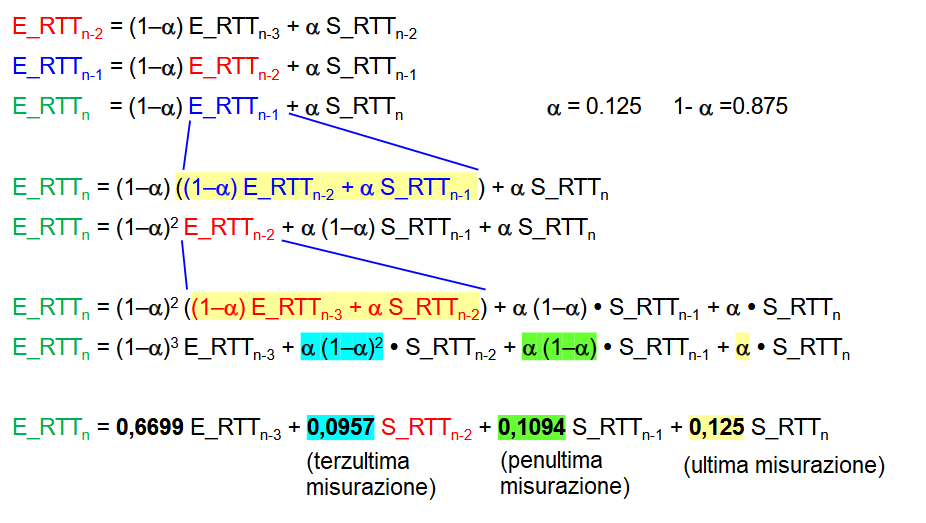
\includegraphics[width=1\linewidth]{./images/rtt.png}
\end{figure}

\subsection{Deviazione del RTT}
La natura variabile dell'RTT ci porta a voler tener conto anche del valore della deviazione standard.
$$
\text{Dev\_RTT} = (1-\beta) \cdot \text{Dev\_RTT} + \beta \cdot |\text{Sample\_RTT} - \text{Estimated\_RTT} |
$$
Un valore tipico è $\beta = \frac{1}{4}= 0.25$. 
\subsection{Risultato finale - Retransmission Time-out}

Dati alla mano, possiamo finalmente stabilire l'RTO, ovvero il valore da dare al timer.

$$
\text{Retransmission Time-Out} = \text{Estimated\_RTT} + 4 \cdot \text{Dev\_RTT}
$$
Con un valore di partenza pari a un secondo (RFC 6298).

\newpage

\section{Timer}
Nonostante RDT stabilisca che ad un pacchetto venga associato un timer, TCP riduce la complessità di gestione gestendo esclusivamente un timer alla volta. Dopo la ricezione dell'ACK dell'$n$-esimo pacchetto, il timer per il segmento $n+1$ non ancora acknowledged viene avviato.

\subsection{Fast-Retransmit}
Per ridurre il tempo di attesa dato dal time-out, si include un'altra condizione per le ritrasmissioni. Questo meccanismo è detto fast retransmit:
se il sender manda tre ACK consecutivi per lo stesso pacchetto mancante (ovvero l'ACK dell'ultimo pacchetto consegnato con successo), viene attivata istantaneamente la ritrasmissione del pacchetto.

\begin{figure}[htp]
	\centering
	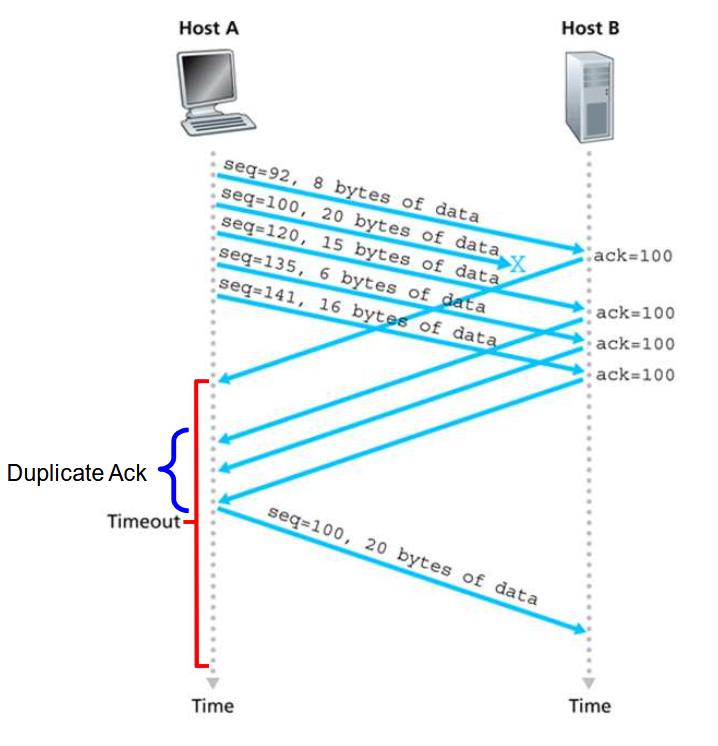
\includegraphics[width=1\linewidth]{./images/fastretransmission.png}
\end{figure}


Questo meccanismo si basa sulla considerazione che, dopo il terzo ACK relativo allo stesso pacchetto non pervenuto, è probabile che questo si sia perso, e vada ritrasmesso. 

\newpage

\section{TCP - Controllo di flusso}
Il problema del produttore-consumatore si ripresenta anche qui: se il Network Layer fornisce dati al buffer del layer di trasporto ad una velocità superiore rispetto a quella con cui l'applicazione può toglierli dal buffer, si corre il rischio di saturarlo.\textbf{ Gestire in maniera consona il flusso è fondamentale} per evitare di dover scartare pacchetti, ed il protocollo TCP implementa dei meccanismi con questo scopo. \textbf{UDP non ha meccanismi equivalenti}.


\subsection{Finestra di ricezione}
Il controllo del flusso viene gestito tramite una variabile chiamata \textbf{Receive Window}, \verb|rwnd|, che specifica al mittente lo spazio libero nel buffer di ricezione del destinatario. Il valore \verb|rwnd| viene aggiornato e trasmesso al mittente tramite un campo dell'header TCP degli ACK.

Quando viene instaurata una connessione TCP, il destinatario riserva un buffer di ricezione denominato \verb|RcvBuffer|, di cui la dimensione può essere configurata tramite le opzioni del socket.

$$
\text{rwnd} = \text{ReceiverBufferSize} - (\text{LastByteReceived} - \text{LastByteRead})
$$

Dove 
\begin{itemize}
	\item \textbf{LastByteReceived} è il numero dell'ultimo byte ricevuto dal livello di rete e inserito nel buffer.
	\item \textbf{LastByteRead} è il numero dell'ultimo byte letto dal buffer dall'application layer.
\end{itemize}

\subsubsection{Circostanza problematica}
Quando il buffer del destinatario si riempie completamente, il receiver manda $\text{rwnd}= 0$, il sender si blocca. Da qui in poi, sia sender che receiver si bloccheranno: come fa il receiver ad aggiornare il sender senza ACK da mandare?
Per risolvere questo problema, il protocollo TCP impone un meccanismo in cui il sender invia dei \textbf{probe packets} contenenti un singolo byte di dati forzando una risposta dal ricevente.

\subsection{Algoritmo di Nagle}
L‘algoritmo di Nagle è una tecnica utilizzata nei protocolli di trasporto, in particolare nel protocollo TCP, per ridurre l‘overhead generato dall‘invio di piccoli pacchetti (ricordiamo che l'RTT è un tempo che viene atteso ad ogni trasmissione di dati). 
Questo è particolarmente utile nelle applicazioni che generano molte trasmissioni di dati di piccole dimensioni, come Telnet, che invia pacchetti di dimensioni minime (tipicamente di 1 byte).
L'obiettivo è \textbf{aggregare dati di piccole dimensioni} nel buffer di trasmissione, \textbf{per inserirli in pacchetti più grandi quando l'RTT della rete è alto}.

\subsubsection{Algoritmo}
\begin{enumerate}
	\item Verificare se ci sono dati tra trasmettere. Se sì, step 2, altrimenti step 3.
	\item Verificare se $\verb|rwnd| \geq MSS$ e che i dati siano $\geq MSS$. Se sì, step 5, altrimenti step 3.
	\item Verifica se stai aspettando un ACK. Se sì, step 4, altrimenti 5.
	\item Accoda i dati da mandare fino alla ricezione dell'ACK, vai a step 5.
	\item Manda i dati, end.
\end{enumerate}

\subsubsection{Pseudocodice}
\begin{verbatim}
	if available_data > 0:
	if window_size >= MSS AND available_data >= MSS:
	send_a_MSS_segment
	else:
	if waiting_for_an_ack == true:
	enqueue_data_in_buffer    /* until an acknowledge is received */
	else:
	send_data
\end{verbatim}

In programmi che richiedono bassa latenza e alta reattività, alcuni sistemi operativi possono disabilitare questo algoritmo tramite l'opzione \verb|TCP_NODELAY| nel socket API.


\section{Connessione TCP}
Il three-way handshake è tra gli aspetti caratterizzanti del protocollo TCP. Andiamo adesso ad analizzarlo nel dettaglio, e ad analizzare perché un two-way handshake non sarebbe funzionale.

\subsection{2-way handshake (un'intuizione inconcludente)}
Prima dell'introduzione del three-way handshake, si è considerato un approccio più semplice (e vicino a quello umano) con un \textbf{two-way handshake}. Si è presto realizzato che un two-way handshake apre le porte a situazioni di \textbf{connessioni half open}. 

\begin{enumerate}
	\item $A$ richiede la connessione a $B$.
	\item $B$ manda un'ACK, apre la connessione
	\item $A$ riceve l'ACK, partecipa alla connessione.
\end{enumerate}
\textbf{E se l'ACK si perde?}

\begin{enumerate}
	\item $A$ chiede la connessione a $B$.
	\item $B$ manda un'ACK e apre la connessione.
	\item L'ACK si perde o il client $A$ crasha. La connessione del server $B$ rimane aperta e in attesa.
\end{enumerate}

Il server $B$ entrerà nello stato \verb|ESTABLISHED|, il client $A$ invece no. Si ottiene quindi una connessione half-open anomala e inutilizzabile.

\subsection{3-way handshake}

Il three-way handshake gestisce queste circostanze tramite un flag \verb|RST| che può essere messo a 1 in un segmento TCP. 

\begin{figure}[htp]
	\centering
	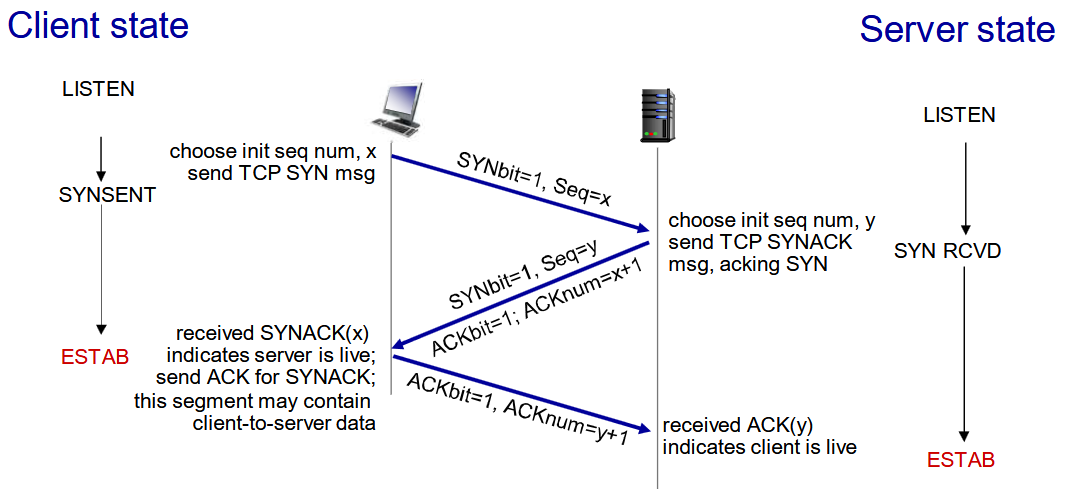
\includegraphics[width=1\linewidth]{./images/3wayhandshake.png}
\end{figure}

\begin{figure}[htp]
	\centering
	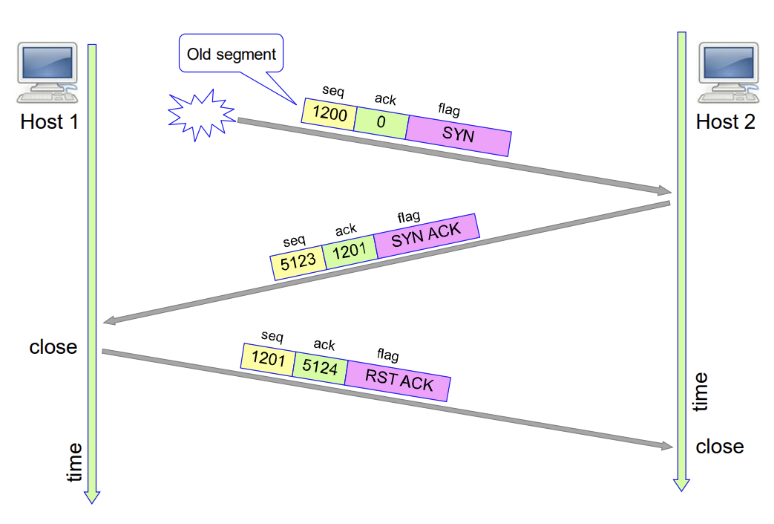
\includegraphics[width=0.75\linewidth]{./images/rstack.png}
\end{figure}


Se l'host $A$ riceve un segmento TCP che \textbf{non riconosce} (e quindi da una connessione che non è stata stabilita con successo, presumibilmente half-open), questo manderà un segmento TCP di \verb|RST ACK| con \verb|RST|=1 per chiedere l'interruzione immediata di questa presunta mezza connessione.

\newpage

\subsection{4-way handshake (2*2-way handshake) per chiusura connessioni}
\underline{La chiusura delle connessioni TCP avviene tramite due 2-way handshake.}\footnote{Si è deciso di sottolineare questa parte in quanto è una puntalizzazione molto importante, soprattutto in sede d'esame.} 
\begin{enumerate}
	\item Il client termina l'invio dei dati: invia segmento con flag \verb|FIN|.
	\item Il server risponde con \verb|ACK|.
	\item Il server è pronto a chiudere la connessione: invia segmento con flag \verb|FIN|.
	\item Il client risponde con \verb|ACK|, chiudendo definitivamente la connessione.
\end{enumerate}
\begin{figure}[htp]
	\centering
	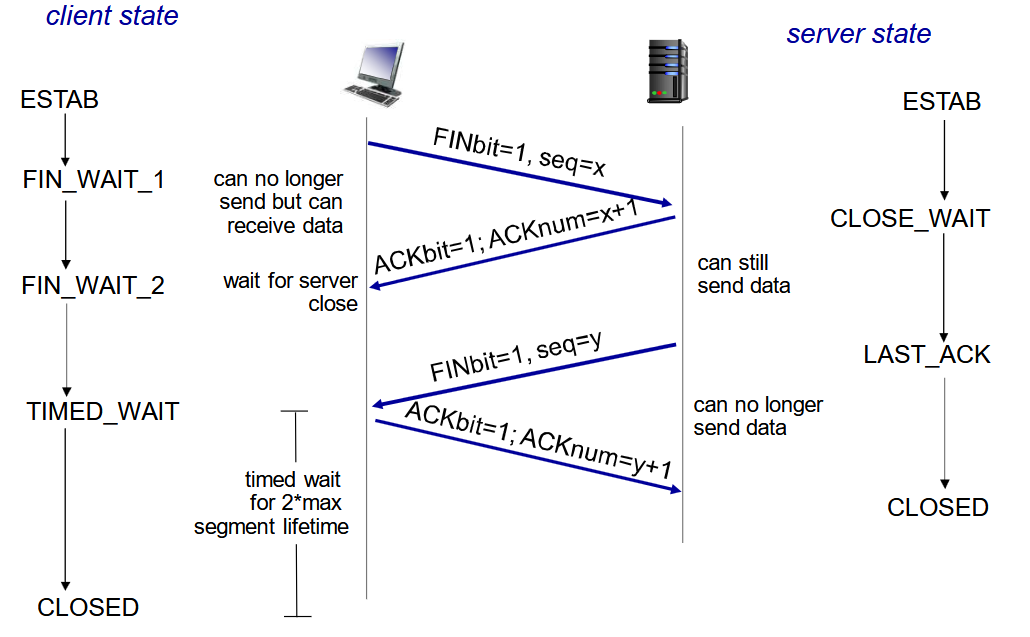
\includegraphics[width=1\linewidth]{./images/4wayhandshake.png}
\end{figure}

Osserviamo che dopo l'invio dell'ultimo \verb|FIN-ACK|, si avvierà un timer \textbf{TIME-WAIT} di tempo pari a 
2 volte tempo di vita massimo di un segmento: ciò darà il tempo ai pacchetti residui nella rete di arrivare (o di far scadere il loro timer) per evitare che vengano ricevuti a connessione ormai chiusa.

\newpage

\section{Controllo della congestione}
La \textbf{gestione delle trasmissioni} è fondamentale per evitare non solo di sovraccaricare i receiver (eventualità gestita tramite il \textbf{controllo del flusso}), ma anche per evitare il sovraccarico della rete, con conseguente congestione.
Il protocollo TCP gode di meccanismi per gestire la congestione, per ridurre la velocità di trasmissione e minimizzare i danni della congestione.

\subsection{Scenario 1 - due mittenti e receiver, router con buffer illimitato}
Nell'analisi della congestione di rete, è importante conoscere dei valori, quali


\begin{itemize}
	\item $\lambda_{\verb|in|}$, frequenza media di invio (dai mittenti).
	\item $\lambda_{\verb|out|}$, la frequenza di arrivo di byte al ricevente.
	\item $R$, la capacità del collegamento condiviso.
\end{itemize}
Quando $\lambda_{\verb|in|}\geq\lambda_{\verb|out|}$, inizia a crearsi congestione.\\
Consideriamo due host mittenti $A$ e
$B$ che inviano a due host destinatari attraverso un router intermedio, e supponiamo che il suo buffer sia illimitato.

\begin{figure}[htp]
	\centering
	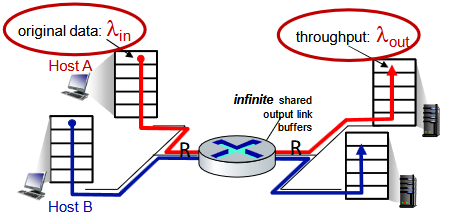
\includegraphics[width=0.5\linewidth]{./images/bufferillimitato.png}
\end{figure}

\begin{itemize}
	\item Se $\lambda_{\verb|in|}\leq \frac{R}{2}$, il router riesce ad inoltrare i pacchetti senza ritardi significativi, e $\lambda_{\verb|out|}=\lambda_{\verb|in|}$. Dividiamo $R$ in due perché abbiamo due host che mandano.
	
	\item Se $\lambda_{\verb|in|} $ aumenta fino a $\frac{R}{2}$, il $\lambda_{\verb|out|}$ massimo si stabilizza su $\frac{R}{2}$.
	
	\item Se $\lambda_{\verb|in|} > \frac{R}{2}$, il throughput non aumenta, ma il numero di pacchetti accodati nel buffer del router cresce senza limite, aumentando il ritardo medio di trasmissione.
\end{itemize}

\newpage

\subsection{Scenario 2 - due mittenti e receiver, un router con buffer limitato}
Quando il buffer di un router è pieno, pacchetti vengono scartati. Di fronte a circostanze simili, TCP prevede ritrasmissione, con conseguente aumento della latenza complessiva aumenta e riduzione frequenza media di invio $\lambda_{\verb|in|}$ diminuisce, in quanto vengono rimandati gli stessi pacchetti. $\lambda_{\verb|in|}'$ tiene conto sia dei dati originali, che delle ritrasmissioni. Distinguiamo ora dei casi di quest scenario.

\begin{enumerate}
	\item \textbf{Nessuna perdita di pacchetti - Perfect Knowledge.}\\
	Se i sender fossero in grado di determinare in anticipo se il router ha spazio disponibile nel buffer, invierebbe un pacchetto solo quando può essere immediatamente elaborato, ottenendo $\lambda_{\verb|in|} = \lambda_{\verb|in|}'$, $\lambda_{\verb|out|}=\lambda_{\verb|in|} \leq \frac{R}{2}$ e zero latenza (perlomeno, causata dal router).
	
	\item \textbf{Ritrasmissione solo per pacchetti persi - Some perfect Knowledge.}\\
	I sender non conoscono lo stato del buffer, e ritrasmettono un pacchetto solo quando hanno la certezza che sia stato perso. Supponendo che $\lambda_{\verb|in|}'=\frac{R}{2}$, $\lambda_{\verb|out|} < \frac{R}{2}$ a causa delle ritrasmissioni.
	
	\item \textbf{Caso reale - duplicati non necessari}.\\
	I sender non conoscono lo stato del buffer, e potrebbero avere un \textbf{timer di ritrasmissione troppo breve}. Questo implica un utilizzo innecessario del buffer del router, della banda e delle risorse di elaborazione. Questo potrebbe addirittura portare ad un throughput di circa $\lambda_{\verb|out|}=\frac{R}{4}$.
\end{enumerate}

\begin{figure}[htp]
	\centering
	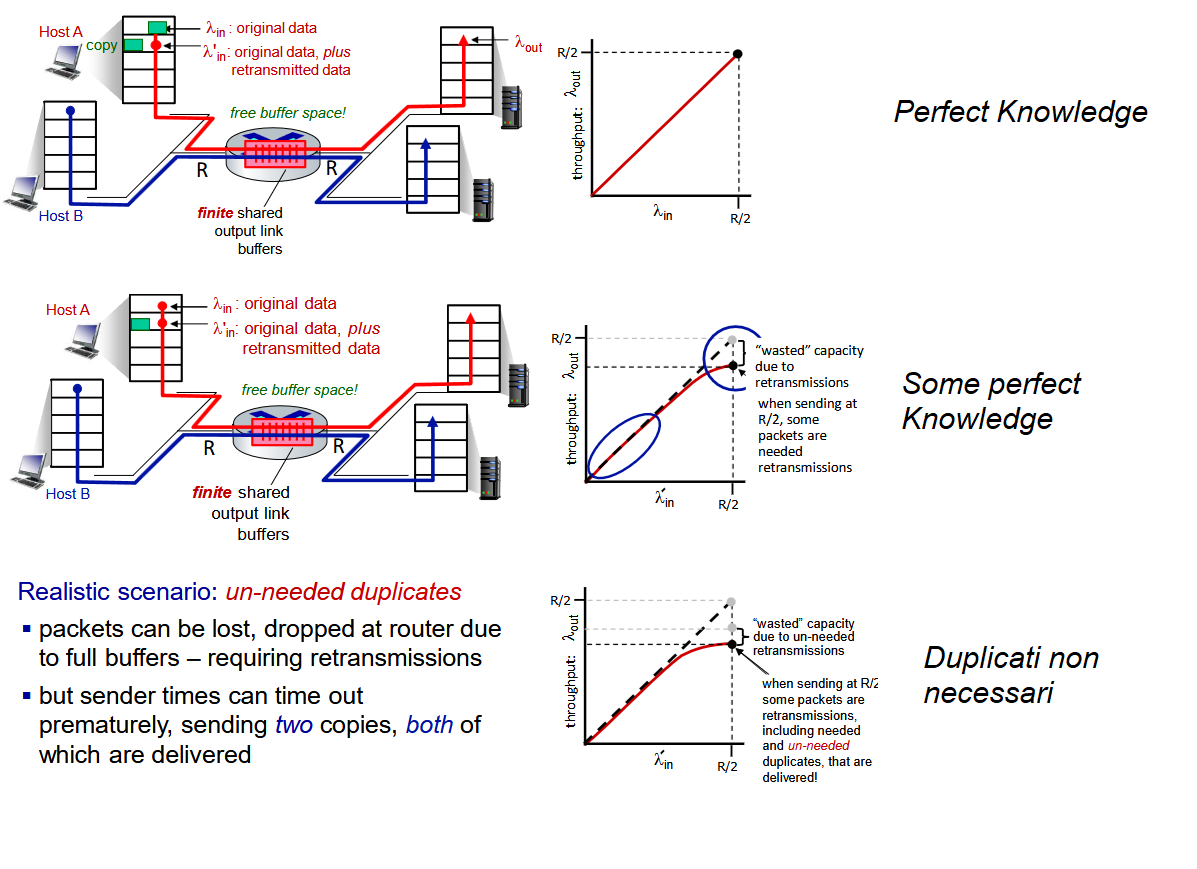
\includegraphics[width=1\linewidth]{./images/limitedbuffer.png}
\end{figure}


\newpage

\subsection{Terzo scenario - quattro mittenti, più router limitati e percorsi}
In questo scenario, quattro mittenti inviano pacchetti su percorsi composti da più collegamenti, condividendo router intermedi. Ogni host utilizza un meccanismo di ritrasmissione basato su timeout, e la rete ha buffer di dimensione finita.

\begin{figure}[htp]
	\centering
	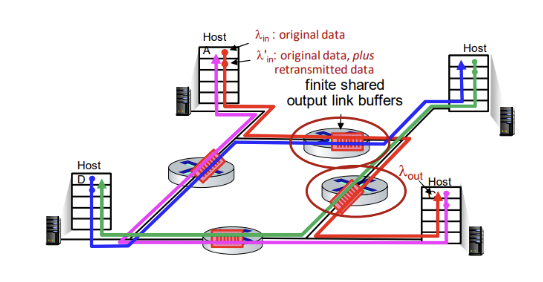
\includegraphics[width=1\linewidth]{./images/4mittentiblahblah.png}
\end{figure}

Abbiamo quattro sender che inviano pacchetti in quattro percorsi con più router, e quindi più possibili percorsi. Ogni router trasmette a capacità $R$. A valori di $\lambda_{\verb|in|}$ piccoli, $\lambda_{\verb|in|} = \lambda_{\verb|in|}'$, non si hanno overflow dei buffer e nemmeno ritrasmissioni. Al crescere del valore di $\lambda_{\verb|in|}$, inizia il rischio di ritrasmissioni, per cui $\lambda_{\verb|in|}' > \lambda_{\verb|in|}$.

\newpage

\section{Meccanismi per gestire la congestione}
Abbiamo quindi capito che la congestione è un fenomeno che si riscontra quando \textbf{il traffico si avvicina o supera la capacità della rete} $R$. Per limitarlo, si opera sulla finestra di trasmissione degli host \verb|cwnd|, aumentando e riducendo in maniera opportuna il numero di pacchetti consentiti contemporaneamente sulla rete (senza aver ricevuto un ACK).
\subsection{Due approcci}
\begin{itemize}
	\item \textbf{Approccio Network-assisted.}\\
	I router forniscono un \textbf{feedback diretto} agli host sender e receiver (di un flusso passante lo stesso router) in merito alla congestione della rete. I router possono fornire il livello di congestione, o esplicitare una \textbf{frequenza di invio}.
	
	\item \textbf{Approccio end-to-end}.\\
	La rete non da alcun tipo di feedback: la congestione è \textbf{dedotta} da ritardi dei pacchetti e ritardi.
\end{itemize}

\subsection{AIMD - Additive Increase Multiplicative Decrease}
Aumento lineare e decremento moltiplicativo della \verb|cwnd|.
\begin{itemize}
	\item Il sending rate è incrementato di 1 MSS a ogni RTT, fino a quando non è individuata una perdita di segmenti.
	\item Dimezza il rate d'invio per ogni evento di perdita segmenti.
\end{itemize}

Ogni incremento viene fatto operando sulla variabile \verb|cwnd|, ovvero la finestra di congestione. 
Il grafico che si ottiene osservando la crescita (e decrescita) del sending rate nel tempo, è detto \textbf{saw-tooth}, dente di sega. Questa tecnica ha tre fasi:
\begin{enumerate}
	\item \textbf{Slow Start}, inizio lento.\\
	Il mittente inizia con una congestion window di 1, ma che cresce, moltiplicata per 2 ad ogni RTT, fino a una soglia stabilita dalla variabile \verb|sstresh|. Oltre quella soglia, si entra in congestion avoidance.
	
	\item \textbf{Congestion Avoidance}.\\
	Superata la \verb|sstresh|, e quindi circa la soglia di $\frac{\text{cwnd}}{2}$, inizia la congestion avoidance: \textbf{la crescita diventa lineare} e \verb|sstresh|= \verb|cwnd|/2.
	\item \textbf{Fast Recovery}.\\
	Congestion avoidance procede normalmente fino a un \textbf{time-out} o tre \textbf{ACK}.
	
	\begin{enumerate}
		\item Se si verifica un time-out, \verb|cwnd| è settato a 1 MSS. 
		\item Se si verifica un triplo ACK, \verb|cwnd| è dimezzato.\\
		Il valore di \verb|cwnd| incrementa di 3 MSS, e quindi \verb|sstresh| = $(\verb|cwnd|+3)/2$.
	\end{enumerate}
	
	
\end{enumerate}


\subsection{Fast Recovery - TCP Tahoe e Reno}

\begin{itemize}
	\item \textbf{TCP-Tahoe.}\\
	Se si perde un pacchetto (individuata da timeout o 3 ACK duplicati), la \verb|sstresh| viene dimezzata, e il cwnd viene azzerato, ripartendo da 1 MSS a priori. Si rientra sempre in slow start dopo qualsiasi evento di perdita.
	\item \textbf{TCP-Reno.}\\
	Se si perde un pacchetto (solo se individuata 3 ACK duplicati), fast recovery! \verb|sstresh| viene dimezzata, e il \verb|cwnd| riparte da un valore $\approx \verb|sstresh|$.\\
	Se si rileva la perdita di pacchetti tramite un \textbf{time-out}, si rientra in \textbf{Slow Start}.
\end{itemize}

TCP Reno è preferibile quando la rete è abbastanza stabile e le perdite di pacchetti sono occasionali: in questo caso, il suo meccanismo di Fast Recovery permette di mantenere buone prestazioni evitando di ritornare sempre allo slow start. TCP Tahoe è invece più adatto in canali altamente congestionati, perché reagisce in modo più drastico alle perdite (tornando sempre a slow start), offrendo un comportamento più prudente e sicuro a scapito dell'efficienza. Insomma, preferire Tahoe a Reno dipende dal canale di trasmissione.

\newpage


\subsection{ECN - Explicit Congestion Notification}
È un approccio alternativo alla gestione della congestione della rete. Sfrutta due bit nel campo \\ \verb|Type Of Service| dell'header IP per comunicare la congestione agli host sender.

\begin{itemize}
	\item Se un router rileva congestione prima di perdere pacchetti, marca il pacchetto con i bit ECN-Capable \verb|ECN = 10| (o \verb|ECN = 01|, sono equivalenti) nell'header IP. Il campo rimane \verb|ECN = 00| se ciò non è supportato.
	
	\item Se la congestione è alta, il router imposta il bit \verb|ECN = 11|
	
	\item Arrivato il pacchetto al destinatario, questo manda un ACK con il bit \verb|ECN = 11|, che significa "Congestion Experienced". In questo modo, il lavoro di notifica è delegato al receiver, e non al router, che manipolerà esclusivamente i bit di quel campo IP. 
	
	\item Il mittente che riceve l'ACK col flag \verb|ECN = 11| abbassa la velocità di invio.
\end{itemize}

\section{TCP Fairness}
TCP è un protocollo fair? Cosa intendiamo per fairness?\\
Si desidera che il controllo della congestione in TCP sia tale che, date $K$ connessioni attraverso la stessa rete con capacità trasmissiva $R$, la \verb|cwnd| di ogni connessione sia $\frac{R}{K}$.

\subsubsection{Dimostrazione della fairness}

Date due connessioni con pari $MSS$ e $RTT$ (e nessun'altra connessione attraverso il collegamento) che operano in \textbf{congestion avoidance}.
Con un throughput massimo pari a $R$, e tenendo a mente che al crescere di uno, diminuisce l'altro, il throughput in una situazione di equilibrio è pari a $\frac{R}{2}$.

\begin{figure}[htp]
	\centering
	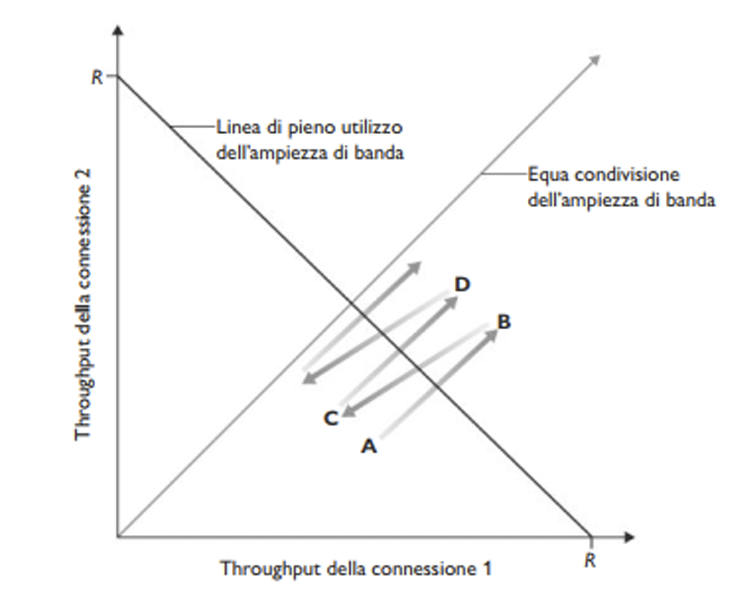
\includegraphics[width=0.65\linewidth]{./images/fairness.png}
\end{figure}

A parità di $RTT$ e $MSS$, gli host \textbf{in congestion avoidance crescono in maniera lineare}: 1 $MSS$ ad ogni $RTT$. Detto ciò, quando la somma del throughput di entrambi gli host supera $R$, questi \textbf{si dimezzano}. Con $x = \text{throughput del primo host}$ e $y = \text{throughput del secondo host}$, e il comportamento di incremento lineare e divisione della finestra di congestione, \textbf{il throughput delle connessioni convergerà sempre alla bisettrice} $x=y$.
In circostanze più vicine a quelle reali, le connessioni con $RTT$ più basso ottengono un throughput maggiore a causa della velocità con cui possono ottenere la connessione. Ricordiamo che l'incremento, nella fase di congestion avoidance, avviene una volta per $RTT$. 

\chapter{Panoramica del Network layer}

\section{Introduzione al Network Layer}
Il compito principale del Network Layer è instradare i pacchetti del livello transport, gestendo il trasferimento e la comunicazione host-to-host.



\subsection{Instradare vs Trasferire}
Sono tra le responsabilità principali del livello di rete, e \underline{non sono la stessa cosa}. Non sono sinonimi, ma solo \textbf{concetti collegati}.

\begin{itemize}
	\item \textbf{Routing, instradamento}.\\
	Definiamo come \textbf{routing} il processo di \textbf{selezione} e \textbf{definizione} di \textbf{cammini} (path, route) per i pacchetti all'interno o tra reti. Indica anche i processi relativi alla \textbf{gestione del traffico} generale \textbf{della rete}. \textit{Routing is the process of selecting and defining paths for IP-packet traffic within or between networks as well as the process of managing network traffic overall.}
	
	\item \textbf{Forwarding, trasferimento}.\\
	Avviene dopo il routing, \textbf{consiste nell'inoltro effettivo dei pacchetti}, secondo i termini stabiliti dal routing.
\end{itemize}

\subsection{Data plane vs Control plane}
La vastità degli argomenti che riguardano il Network Layer, ci spingono a suddividere la discussione tra \textbf{data plane} e \textbf{control plane}.

\begin{itemize}
	\item \textbf{Data plane.}\\
	Il dataplane è la parte del router o dello switch che si occupa del trasferimento effettivo dei pacchetti, inoltrandoli da un’interfaccia all’altra secondo i termini stabiliti del control plane. Opera in modo veloce e automatico, spesso in hardware. È quindi il responsabile del forwarding!
	
	\item \textbf{Control plane.}\\
	Il control plane è responsabile di prendere decisioni sul percorso dei pacchetti, costruendo e aggiornando le tabelle di routing seguendo dei protocolli dedicati. Gestisce la logica e la configurazione della rete. È chiaramente il responsabile del routing.
\end{itemize}

\newpage

\section{Routing}

Esistono due approcci differenti:
\begin{itemize}
	\item \textbf{Traditional Routing Algorithms.}\\
	Effettuato dai singoli router, senza una visibilità globale, ma dei propri neighbours. È una struttura distribuita, più resistente della prossima soluzione, ma più lenta. Ogni router ha al proprio interno una tabella d'instradamento, cui valoi vengono aggiornati di volta in volta.
	\item \textbf{Software Defined Network.}\\
	È un'architettura centralizzata esterna, che sa tutto della rete. Ottiene path migliori e più velocemente, ma se l'SDN va giù, il sistema crolla. Inoltre, riceverà un altissimo numero di richieste non-distribuite, in quanto, in questo tipo di architettura, è proprio il controller remoto a calcolare e distribuire le tabelle di inoltro.
	
\end{itemize}
\subsection{Self-Organizing-Routing}
Scambiandosi informazioni, ottengono una visione generale della rete. Determinano un routing migliore tramite algoritmi quali Bellman-Ford e Dijkstra. Questi algoritmi sono rinforzati tramite euristiche, tecniche AI e di reinforcement learning. Andremo ad approfondire questa parte affrontando il control-plane. 

\subsection{SDN - Software Defined Networking}
Il control plane è centralizzato in un remote controller.\\
Conosce tutta la topologia della rete, e prende decisioni sui percorsi che devono seguire i pacchetti, sa come aggiornare le tabelle di inoltro nei router. Manda istruzioni ai router sull'instradamento e riceve aggiornamenti dai router sul traffico. Il control agent (CA) è un modulo che gira sui router che permette di comunicare col Remote Controller. Il remote agent non agisce mai in autonomia dal remote controller.

\subsection{Virtual Circuit Service, circuito virtuale}
È una modalità di commutazione in cui, tra due peer, viene costruito un \textbf{circuito virtuale} in fase di connessione (secondo i soliti metodi di routing). L'inoltro dei pacchetti \textbf{di quella connessione} procederà \underline{esclusivamente} sul \textbf{percorso stabilito}. In queste circostanze è chiaro che i router \textbf{non siano state-less}: manterranno infatti delle informazioni di routing relative a quella connessione. Un qualsiasi \textbf{malfunzionamento} dei router nel percorso, implica una \textbf{riconnessione da zero}. In compenso, il \textbf{controllo della congestione} è molto più \textbf{semplice}. 

\subsection{Packet Switching, commutazione di pacchetto}
La modalità a circuito virtuale è molto diversa alla più usata modalità di \textbf{packet switching} (ovvero della \textbf{commutazione a pacchetto}) in cui tutti i \textbf{pacchetti}, anche della stessa connessione, sono \textbf{inoltrati separatamente} sulla base delle informazioni contenute negli \textbf{header}. Instradano ogni pacchetto secondo le proprie tabelle di routing, e \underline{non pensando ad un circuito fisso tra due host}.


\subsection{Router}
Al giorno d'oggi sono dei "mini-stack ISO/OSI", cui livello più alto è il transport.\\
Attualmente, i router contengono un \textit{firmware}\footnote{Sono programmi scritti nella memoria flash, solitamente in linguaggio di basso livello (Assembly, C di basso livello). Sono software che la CPU può eseguire direttamente grazie al program counter. All'accensione del dispositivo, il codice viene copiato nella SRAM, e la CPU lo esegue. Questi firmware sono velocissimi, ed è il motivo per cui rispondono alle esigenze dei router.} nella propria memoria flash.
\begin{itemize}
	\item Esamina gli \textbf{header} dei datagrammi IP che gli passano attraverso.
	\item Sposta i datagrammi \textbf{dalla porta di input} a quella di \textbf{output} per trasferire i datagramma nel path stabilito. Effettuano un \textbf{forward} dei pacchetti.
\end{itemize}

\subsection{Indirizzamento logico}
Consiste nell'assegnamento di \textbf{indirizzi logici} ai dispositivi (tramite indirizzi \textbf{IP}) per \textbf{identificare} in modo univoco ogni \textbf{nodo nella rete}.

\section{Frammentazione e riassemblaggio}
I \textbf{datagrammi IP troppo grandi} per il router devono essere \textbf{frammentati e riassemblati al mittente} per renderne possibile il trasferimento. Questo è uno dei compiti del data plane del Network Layer (la MTU dell'Ethernet è di 1500 byte). In dei casi, si vorrebbe poter avere la possibilità di controllare se permettere o meno la frammentazione. Questo è ottenuto tramite dei flag opportuni dell'header IPv4 (Don't Fragment e More Fragment). Scopriremo anche che IPv6 non permette la frammentazione da parte dei router intermedi.


\section{Modelli di servizio di rete}
In inglese, \textbf{Network Service Model}.
Stabiliscono le caratteristiche del trasporto dei datagrammi da host a host.\\
I servizi possono fare riferimento ai singoli pacchetti, quali
\begin{itemize}
	\item \textbf{Consegna garantita}.
	\item Consegna garantita \textbf{entro $n$ millisecondi}.
\end{itemize}
O a interi flussi di datagrams, come
\begin{itemize}
	\item \textbf{Consegna} dei datagrammi \textbf{in ordine}.
	\item \textbf{Bandwidth minima} garantita.
	\item \textbf{Maximum jitter}, garantisce che la variazione massima tra i ritardi dei pacchetti.
\end{itemize}

Su Internet, garantire questi servizi è semplicemente utopia. In campo militare o finanziario, alcuni di questi servizi devono essere garantiti. Nelle reti degli ATM, viene usato un servizio di \textbf{Available Bit Rate}. Garantisce una bandwidth minima utilizzando la banda di rete disponibile.

\subsection{Internet Service Model - Best Effort}
In Internet, le \textbf{garanzie} in termini \textbf{di reliability} sono affidate al \textbf{livello di trasporto}, tramite \textbf{RDT} e \textbf{meccanismi vari del TCP}. Il network, nel caso di Internet, non si occupa di assicurare i servizi appena esposti, ma di offrire dei meccanismi di instradamento e inoltro dei pacchetti per i livelli superiori.

\subsubsection{Best Effort - Complice della popolarità di Internet?}
La semplicità dei meccanismi dietro ai servizi \textbf{best-effort di Internet}, \textbf{ha indubbiamente permesso} a quest'ultimo di \textbf{espandersi a macchia d'olio}.\\
Con una larghezza di banda sufficientemente ampia, le applicazioni funzionano piuttosto bene la maggior parte delle volte. \textbf{Good enough!}

\chapter{Network Layer - Piano dei dati}

\section{I router}
I router sono sicuramente i dispositivi più responsabili dell'instradamento e dell'inoltro all'interno delle reti. Sono quindi un elemento fondamentale per il Network Layer, e quindi da studiare approfonditamente.

\subsection{Elementi principali di un router}
\begin{figure}[htp]
	\centering
	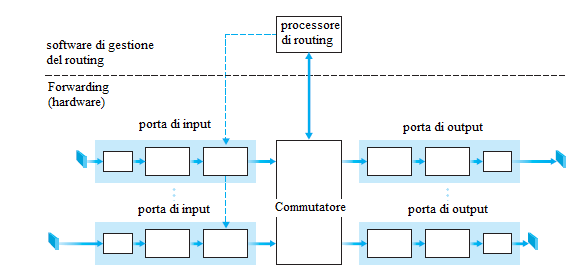
\includegraphics[width=0.75\linewidth]{./images/router.png}
\end{figure}

\begin{itemize}
	\item \textbf{Porte di ingresso.}\\
	Sono le \textbf{terminazioni a livello fisico} per i collegamenti in ingresso al router. Inoltre, è sempre nella porta d'ingresso che si effettua la \textbf{decisione di forwarding}. Ogni porta contiene infatti una copia della tabella di routing.
	In questo caso, il termine "porta" fa riferimento a interfacce fisiche d'input (e output), ben diversi dalle porte software dei processi e dei socket.
	
	\item \textbf{Struttura di commutazione.}\\
	Connette fisicamente le porte d'ingresso a quelle di uscita. Una sorta di rete interna al router. È una struttura che deve permettere una \textbf{commutazione ad alta velocità}, sfruttando la tabella di forwarding fornita dal piano di controllo.
	
	\item \textbf{Porte di uscita.}\\
	Memorizzano i pacchetti che provengono dalla struttura di commutazione e li trasmettono sul collegamento d'uscita. Nei collegamenti bidirezionali, la porta d'uscita è accoppiata alla porta d'ingresso sulla stessa scheda di collegamento (detta line card).
	
	\item \textbf{Processore d'instradamento.}\\
	Esegue le funzioni del piano di controllo. Il funzionamento varia tra i router tradizionali e quelli SDN\footnote{Software Defined Networking}. Nei primi, il processore d'instradamento gestisce le tabelle di inoltro. Nel secondo caso, si occupano di gestire la comunicazione con il controller remoto.
\end{itemize}

In un router, mentre il processore d'instradamento è principalmente software, le porte di ingresso, di uscita e le strutture di commutazione, sono gestite da hardware dedicato.
In questo modo, è possibile ottenere le performance richieste dalla rete, operando in lassi temporali dell'ordine dei millisecondi. 

\newpage
\subsection{Porte d'ingresso del router}
Le porte d'input svolgono sia una funzione di terminazione (elettrica) per il livello fisico, sia l'elaborazione per il livello di collegamento.\\
Usando le informazioni della tabella d'inoltro, viene determinata la porta d'uscita dei pacchetti (attraverso la struttura di commutazione).\\
La tabella di inoltro viene elaborata e aggiornata dal processore di instradamento (control plane), e viene copiata e mandata a line card e porte d'ingresso, in modo da permettere alle porte d'ingresso di prendere decisioni senza invocare il processore d'instradamento centralizzato.

\subsection{Tabelle d'inoltro e destination-based forwarding}
\begin{figure}[htp]
	\centering
	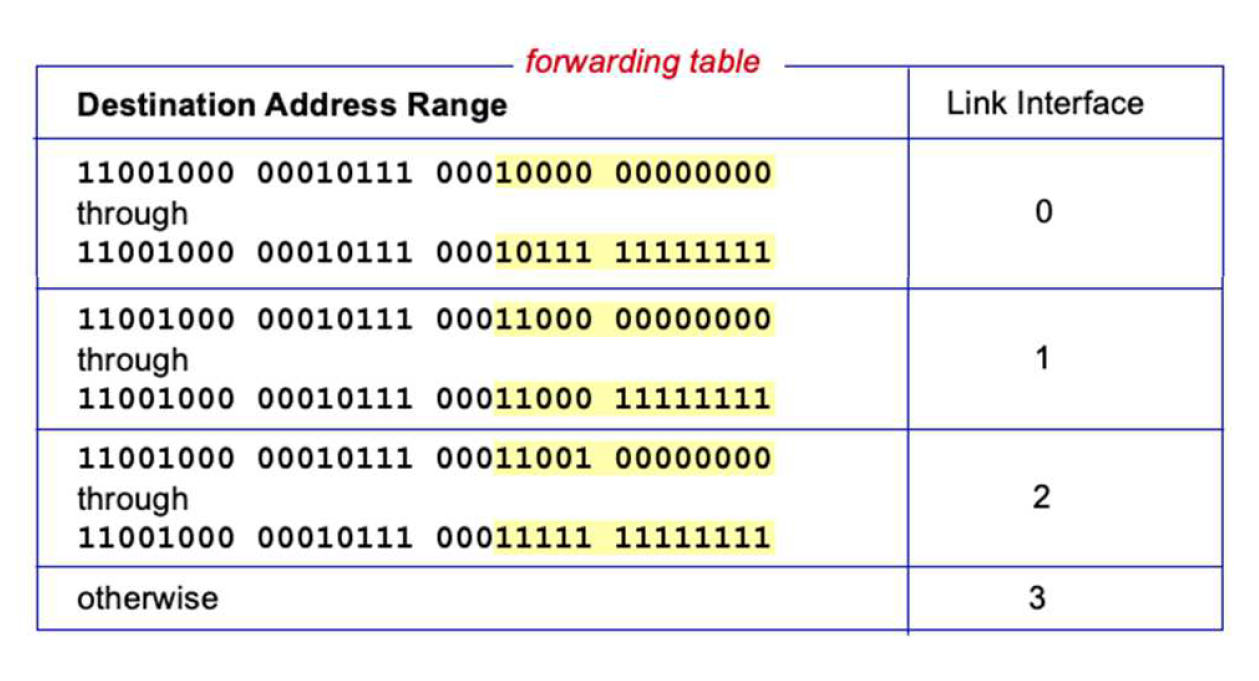
\includegraphics[width=0.75\linewidth]{./images/tabellainoltro.png}
\end{figure}
La decisione della porta d'inoltro può avviene tramite un processo di longest-prefix-matching (in italiano, corrispondenza a prefisso più lungo). L'indirizzo di destinazione viene confrontato con una lista di prefissi associati a dei collegamenti: quello dal match migliore, detterà la porta d'uscita dei pacchetti.
\begin{figure}[htp]
	\centering
	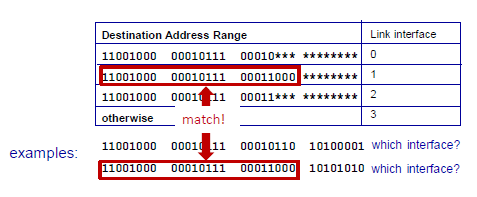
\includegraphics[width=0.75\linewidth]{./images/prefix.png}
\end{figure}

\subsubsection{Ternary Content Addressing Memory}
Lo string matching non è un problema semplice, nemmeno nel caso dei prefissi: soprattutto in un contesto come quello dei router, che devono operare ad altissime velocità, risulta fondamentale implementare questi meccanismi in maniera hardware.\\
Entrà quindi in giorno la TCAM. La Ternary Content-Addressable Memory (TCAM) è un tipo specializzato di memoria ad alta velocità che può cercare all'interno del suo intero contenuto in un solo ciclo di clock. Il termine ternario si riferisce alla capacità della memoria di memorizzare e interrogare i dati utilizzando tre diversi valori: 0, 1 e X (perfetta per i prefissi!). La TCAM è utilizzata nel contesto dei router per memorizzare le tabelle di ricerca degli indirizzi, ed effettuare in tempo costante il controllo di tutti i prefissi, per trovare il prefisso dal matching migliore con l'indirizzo di destinazione fornito.

\newpage

\subsection{Struttura di commutazione}
È il cuore del router, mezzo tramite cui i pacchetti vengono commutati (inoltrati) dalla porta d'ingresso alla porta d'uscita. La commutazione può essere ottenuta attraverso varie strutture di commutazione:
\begin{itemize}
	\item \textbf{Commutazione in memoria.}\\
	Avviene sotto il controllo diretto della CPU (ovvero il processore di instradamento), con le porte di ingresso e uscita trattate come dispositivi di I/O. I primi router usavano questa struttura, che con una determinata bandwidth della memoria tale da permettere di leggere e scrivere $B$ pacchetti per unità di tempo, il throughput complessivo d'inoltro deve necessariamente essere $< \frac{B}{2}$. Le operazioni di inoltro su due porte differenti non potevano nemmeno avvenire in contemporanea, a causa dell'impossibilità di effettuare due operazioni di lettura/scrittura contemporaneamente.\\
	Alcuni router attuali effettuano commutazione in memoria, ma la ricerca dell'indice e la memorizzazione del pacchetto nella locazione di memoria opportuna avviene sulle line card di ingresso. Alcuni di questi router, somigliano a sistemi multiprocessore a memoria condivisa.
	
	\item \textbf{Commutazione tramite bus.}\\
	In questo approccio le porte di ingresso trasferiscono un pacchetto direttamente alle porte di uscita tramite un bus condiviso e senza intervento dal processo di instradamento.\\
	Si ottiene aggiungendo al pacchetto un'etichetta di commutazione: questa indicherà la porta locale di output da cui dovrà uscire. Il pacchetto verrà ricevuto da tutte le porte d'output, ma solo la porta corrispondente lo raccoglierà. Un difetto di questo sistema? Solo un pacchetto alla volta può occupare il bus: la larghezza di banda della commutazione sarà limitata da quella del bus. Più pacchetti da commutare saranno messi in coda. È comunque un valido sistema per router in reti di accesso e aziendali. Gli switch Cisco della serie 5600 hanno una bandwidth di $32 \ Gbps$.
	
	\item \textbf{Commutazione attraverso rete di interconnessione.}\\
	Usa una rete di interconnessione più sofisticata, con una matrice di commutazione (\textit{crossbar switch}): consiste in $2n$ bus che collegano $n$ porte di ingresso a $n$ porte d'uscita. Ogni bus verticale interseca tutti i bus orizzontali a un punto d'incrocio che può essere aperto o chiuso dal controller della struttura di commutazione in qualsiasi momento.
	Quando un pacchetto che entra dalla porta $A$ deve essere inoltrato alla porta d'uscita $Y$, viene chiuso l'incrocio tra i bus $A-Y$.\\ Analogamente, questo avviene per l'entrata $B$ e l'uscita $X$. Quando sono coinvolte porte d'uscita differenti, i pacchetti possono essere trasferiti in parallelo, altrimenti si accoderanno alla porta d'output.\\
	Architetture più sofisticate utilizzano strutture per la commutazione a più stadi, che permette di spostare in contemporanea pacchetti da più porte verso una sola porta.\\
	Tra questi, i router Cisco CRS usano un'ulteriore strategia a $n$ strutture di commutazione: il pacchetto da trasferire viene suddisivo in $k$ frammenti (chunk). Ogni frammento verrà trasferito attraverso una struttura, mentre la porta di uscita si occuperà del riassemblaggio. Questo permette di avere ancora $n-k$ strutture di commutazione libere per eventuali altri pacchetti.
	\begin{figure}[htp]
		\centering
		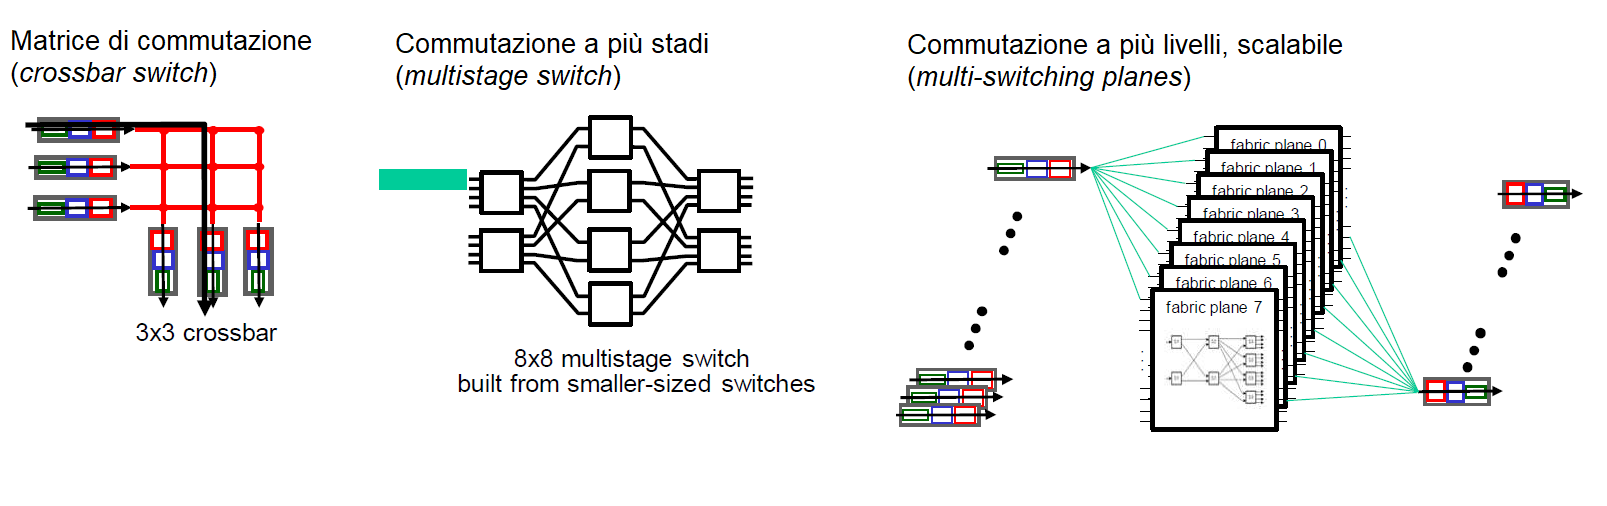
\includegraphics[width=1\linewidth]{./images/commutationstructure.png}
	\end{figure}
\end{itemize}

\newpage

\subsection{Accodamento}
L'accodamento è un fenomeno che, se non viene gestito correttamente, può portare alla saturazione totale della memoria e alla perdita di pacchetti.

\subsubsection{Accodamento alle porte d'ingresso}
Quando la struttura di commutazione non è sufficientemente rapida rispetto alle linee di ingresso, è proprio nelle porte d'input che si ha accodamento. I pacchetti sono serviti con un meccanismo FCFS (\textit{First-Come-First-Served}).\\
Abbiamo già detto che pacchetti che devono uscire da porte differenti possono essere trasferiti in parallelo. Quando due pacchetti devono uscire dalla stessa porta, uno dei due dovrà attendere. Supponiamo di avere due porte $A, B$ e due uscite $X,Y$. Supponiamo arrivino due pacchetti $x_1, x_2$ per $X$, uno dalla porta $A$, uno dalla porta $B$. Se $x_1$ va verso la porta $X$, $x_2$ andrà in coda. Un eventuale pacchetto $y_1$ che dalla porta $B$ vuole andare alla porta $Y$ soffrirà di un fenomeno noto come \textbf{HOL blocking}, proprio a causa dell'accodamento di $x_2$.

\subsubsection{Accodamento alle porte d'uscita}
Supponiamo che $R_{switch}= N \cdot R_{line}$, ovvero che il tasso di trasferimento della struttura sia $N$ volte più veloce della velocità di trasferimento nelle linee d'input e output.\\
Nel tempo richiesto per ricevere o trasmettere un pacchetto, una porta potrebbe ricevere fino a $N$ pacchetti, causando la formazione di una coda nella porta d'uscita. Il numero di pacchetti nella coda d'uscita è direttamente proporzionale alla dimensione del buffer di quella porta. Quando il buffer è saturo e arriva un ulteriore pacchetto, si deve stabilire se effettuare un \textbf{drop-tail}, scartando il nuovo pacchetto, o rimuoverne uno o più di uno tra quelli già in coda, a favore del nuovo arrivato.

\subsubsection{Quanta memoria assegnare al buffer}
\verb|RFC 3439| stabiliva che la grandezza del buffer $B$ dovesse essere uguale al round trip time medio $RTT$ moltiplicato per la calacità del link $C$.\\
Un esempio? Un collegamento con bandwidth $10 \ Gbps$ con un RTT di $250 \ ms$ necessiterebbe di un buffer $B$ pari a
$$
B = RTT \cdot C = 10 \ Gbps \cdot 250 \ ms = 10 \cdot 0,25 = 2,5 \ Gbit
$$
Anche se recenti studi teorici, suggeriscono che, con un numero $N$ di flussi TCP indipendenti, la quantità di buffer necessaria sia 
$$
B \approx RTT \cdot \frac{C}{\sqrt{N}}
$$
Buffer troppo grandi aumentano i delay (soprattutto nei router di casa, che non gestiscono in maniera ottimale la coda, causando \textbf{bufferbloat}).
RTT troppo lunghi rendonono i mittenti TCP meno reattivi. Alcuni controlli della congestione basati sul ritardo permettono di mantenere la linea occupata, senza riempire il buffer.

\begin{figure}[htp]
	\centering
	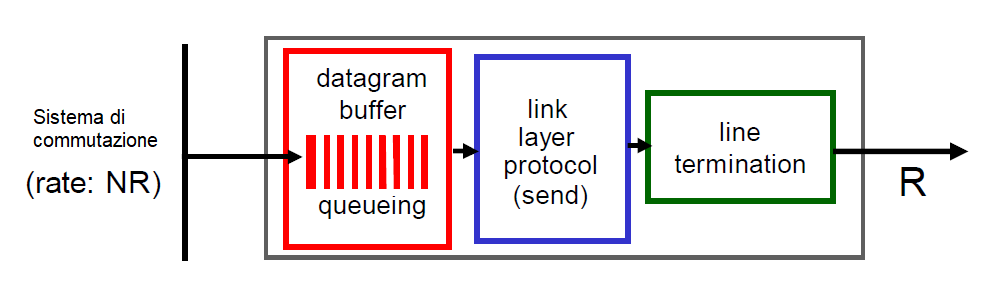
\includegraphics[width=0.75\linewidth]{./images/portaduscita.png}
\end{figure}


\newpage

\subsection{Packet discarding policy}

\subsubsection{Tail drop}
Quando la coda è piena, \textbf{i pacchetti in arrivo vengono scartati a priori}, senza considerare priorità o tipologia del traffico. Droppare pacchetti in questo modo potrebbe causare \textbf{burst di drop}.

\subsubsection{Priority queueing}
Il buffer è diviso in più code, ognuna con priorità diversa. I pacchetti vengono etichettati con un livello di priorità (o può essere stabilita dal router). In questo modo, i pacchetti ad alta priorità non saranno scartati, quando sono presenti in coda altri pacchetti a priorità più bassa. 

\subsection{Scheduling dei pacchetti}
Come determiniamo l'ordine con cui trasmettere i pacchetti su una determinata porta d'uscita? 

\subsubsection{FIFO (o FCFS)}
First-In-First-Out o First-Come-First-Served. Il paradigma più semplice: chi prima arriva, prima viene mandato.

\subsubsection{Priority scheduling}
Estende il modello FIFO-FCFS con un meccanismo di priorità: vengono definite più code per varie classi di priorità. Ad esempio, con due code (alta e bassa priorità), è possibile distribuire i pacchetti dei servizi in tempo reale (o informazioni di gestione di rete) e i pacchetti di servizi non in tempo reale. Le singole code seguono solitamente il principio FIFO, ma, date due code non vuote, verrà sempre preso il pacchetto nella coda ad alta priorità.

\subsubsection{Round-Robin}
Vengono di nuovo suddivisi i pacchetti in classi, non più (mandatoriamente) suddivise per priorità di servizio. A turno, ogni coda viene servita: viene trasmesso un pacchetto di classe $1$, poi $2$, fino alla $n$-esima classe. Poi di nuovo $1$, $2\dots n$. Col \textit{work-conserving round robin}, quando una coda è vuota, viene del tutto saltata dalla selezione.
%Adoro i bambini 

\subsubsection{WFQ - Weighted Fair Queuing}
Accodamento equo ponderato. È un Round Robin generalizzato, in cui ogni classe può ricevere un servizio differenziato. Ogni classe $i$ avrà un peso $w_i$. Il WFQ assicura che l'$i$-esima classe di pacchetto riceva sempre $\frac{w_i}{\sum{w_i}}$, dove $\sum w_i$ indica la somma tra i pesi di tutti i servizi.\\
Non dimentichiamo, tuttavia, che i pacchetti sono unità discrete e che la loro trasmissione non può essere interrotta. Questo rapporto è quindi indicativo.

\section{I protocolli del livello di rete}
\begin{itemize}
	\item \textbf{IP protocol}.\\
	E la formattazione dei pacchetti, l'addressing e le convenzioni relative alla gestione dei pacchetti.
	\item \textbf{Path-selection algorithm.}\\
	Che gestiscono l'instradamento dei pacchetti.
	\item \textbf{Protocollo ICMP}.\\
	Dedicato agli errori e ai segnali dei router.
\end{itemize}

\newpage

\section{IPv4 - Internet Protocol v4}

\subsection{Indirizzo IP}
Un indirizzo IP è un codice logico (non fisico, non 1-a-1) associato ad un host connesso a una rete che usa il protocollo Internet. 

\subsubsection{Classi di indirizzi IP}
Un sistema che permetteva di distinguere vari tipi di indirizzi IP è quello per classi.
\begin{itemize}
	\item Indirizzi di classe A.\\
	From \verb|1.0.0.0| to \verb|127.255.255.255|.
	Il primo byte identifica la rete, gli altri gli host.
	\item Indirizzi di classe B.\\
	From \verb|128.0.0.0| to \verb|191.255.255.255|.
	I primi due byte identificano la rete, gli ultimi due gli host.
	\item Indirizzi di classe C.\\
	From \verb|192.0.0.0| to \verb|223.255.255.255|
	I primi tre byte identificano la rete, l'ultimo gli host.
	\item Indirizzi di classe D (multicast).\\
	From \verb|224.0.0.0| to \verb|239.255.255.255|. Sono riservati agli indirizzi multicast. Permettono quindi di trasmettere la stessa informazione a più dispositivi contemporaneamente senza dover duplicare l'informazione.
	\item Indirizzi di classe E (riservati).\\
	Riservati per usi futuri.
	From \verb|240.0.0.0|
\end{itemize}

\subsubsection{Alcuni indirizzi specifici}
Questi indirizzi sono riservati a delle funzioni specifiche.
\begin{itemize}
	\item \verb|0.0.0.0| - This Host, usato su un host cui indirizzo non è ancora stato specificato (ma solo in IPv4, non in IPv6, che usa un indirizzo IP basato sul MAC Address. Guarda EUI-64, pagina 81).
	\item \verb|255.255.255.255| - Broadcast relativo alla propria subnet.
	\item \verb|127.0.0.0 - 127.255.255.255| - Localhost, riferimento a se stesso.
	\item \verb|10.0.0.0 - 10.255.255.255| - Private IP.
	\item \verb|169.254.0.0 - 169.254.255.255| - Automatic Private IP Addressing (APIPA), usate per risolvere problemi relativi al DHCP.
\end{itemize}

\subsection{Assegnamento degli indirizzi IP}
\begin{enumerate}
	\item Inizialmente, questo compito era affidato alla \textbf{IANA} (Internet Assigned Numbers Authority), ai tempi di Arpanet.
	\item Nel 1992, sono stati creati i \textbf{RIR} (Regional Internet Registers), creati per gestire gli indirizzi e domini per ogni area assegnata
	\item Nel 1998 un'associazione non-profit chiamata \textbf{ICANN} (Internet Corporation for Assigned Network and Numbers) è stata fondata per coordinare tutti i RIR del mondo.
\end{enumerate}

\subsubsection{I RIR attuali}
\begin{itemize}
	\item APNIC - Asia Pacific Network Information Center
	\item ARIN - American Registry for Internet Numbers
	\item LACNIC - Latin American and Caribbean Internet Addresses Registry
	\item RIPE NCC - Réseaux IP Européens Network Coordination Centre
	\item AFRINIC - African Regional Internet Registry
\end{itemize}

I RIR sono responsabili per i Local Internet Registries, che gestiscono gli indirizzi a livello locale. Un esempio è il GARR-LIR\footnote{GARR è il nome della rete italiana a banda ultralarga dedicata alla comunità dell'istruzione, della ricerca e della cultura (NREN), oltre che del consorzio che la gestisce.}. I RIR forniscono vari set di indirizzi (statici e dinamici) agli ISP.


\newpage

\subsection{Formattazione dei Datagram IPv4}
Questa è la struttura di un datagramma IPv4. Osserviamo i singoli campi

\begin{figure}[htp]
	\centering
	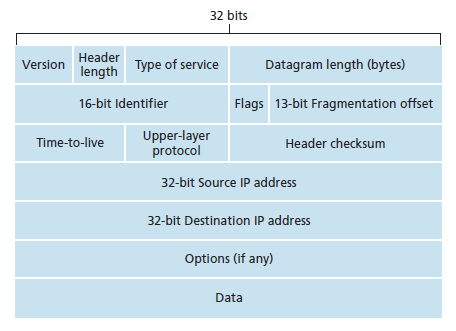
\includegraphics[width=0.75\linewidth]{./images/ipv4datagram.png}
\end{figure}


\begin{itemize}
	\item \textbf{Version.}\\
	Indica la versione di IP usata dal datagramma. È fondamentale per capire come interpretare il pacchetto IP. 4 bit. 
	\item \textbf{Internet Header Length.}\\
	Indica la lunghezza dell'header del pacchetto IP, ovvero l'offset del campo dati, che varia da 5 word a 15 word (ovvero da 20 a 60 byte). Ciò dipende dalla presenza o meno del campo \textit{Options}.
	\item \textbf{Type of Service.}\\
	Da informazioni relative al servizio fornito, stabilendone la priorità.
	
	\item \textbf{Datagram length.}\\
	Indica la dimensione in byte dell'intero pacchetto. Include quindi header e dati. 16 bit.
	
	\item \textbf{ID, Flags e Fragmentation Offset.}\\
	Ne parleremo meglio dopo. Rispettivamente 16, 3 e 13 bit.
	
	\item \textbf{TTL - Time To Live.}\\
	Specifica il tempo di vita massimo di un pacchetto. Per qualsiasi problema nella rete, un pacchetto potrebbe persistere nella vita per un quantitativo spropositato di tempo. Potrebbe essere addirittura una cosa voluta per un possibile attacco hacker. Il time to live ovvia a questo problema definendo un numero di salti, nel momento in cui il pacchetto viene mandato in rete: ogni salto attraverso un router implica un decremento. Usa 8 bit.
	
	\item \textbf{Protocol.}\\
	Specifica il protocollo del transport layer. 4 bit.
	
	\item \textbf{Header checksum.}\\
	8 bit dedicati alla somma di controllo. Un pacchetto cui header risulta corrotto, viene scartato. Le operazioni sono di natura logica o matematica, ed il controllo è fatto a ogni router.
	
	\item \textbf{Options.}\\
	Quasi inutilizzate.
	
	\item \textbf{Source IP e Destination IP.}\\
	32 bit ciascuno, 64 in totale. Sono due campi separati.
\end{itemize}

\subsection{Un problema: la frammentazione}
Alcuni campi che non abbiamo ancora affrontato, sono quelli relativi alla frammentazione. Quando un datagramma IP viene frammentato in più datagrammi IP più piccoli, queste informazioni permettono la ricostruzione del frammento originale a destinazione.
La frammentazione avviene quando un router ha MTU (Max Transfer Size) tale da non consentire il trasferiremnto dell'intero datagramma IP.
\begin{itemize}
	\item \textbf{ID.}\\
	16 bit, identificano un insieme di pacchetti IP che (presumibilmente) ricostruiranno un pacchetto originale.
	\item \textbf{Flags.}\\
	3 bit, 2 usati. I flags sono \verb|DF - Don't Fragment|, $=1$ "Non frammentare mai. Al massimo, scarta."\\
	\verb|MF - More Fragments|, $=1$ "Questo non è l'ultimo frammento".
	\item \textbf{Offset.}\\
	13 bit, indica dove inizia il frammento rispetto all'inizio del pacchetto originale, espresso in unità da 8 bit. Permette di ricostruire in maniera opportuna i pacchetti frammentati.
\end{itemize}

Questo compito non spetta solitamente ai router, i quali ricordiamo occuparsi principalmente di forwarding. Una corruzione dei dati di frammentazione può avere gravi conseguenze in fase di ricostruzione.

\begin{itemize}
	\item \textbf{Offset alterato} - il ricongiungimento dei pezzi non può essere eseguito correttamente.
	\item \textbf{ID alterato} - un frammento potrebbe cambiare pacchetto di appartenenza.
	\item \verb|MF=1 -> MF=0| - un frammento che non è l'ultimo potrebbe essere considerato l'ultimo.
\end{itemize}

\subsubsection{Esempio di frammentazione}
Dato un pacchetto con 4000 byte e un router con MTU di 1500 byte (come Ethernet).
\begin{itemize}
	\item Se il frammento arriva con il flag $\verb|DF|= 1$, viene scartato
	\item Con $\verb|DF|=0$ si procede alla frammentazione.
\end{itemize}

Vediamo come procederebbe la frammentazione.

\begin{enumerate}
	\item Il primo frammento viene mandato con $\verb|MF|=1$ con offset a 0. Il segmento mandato è di 1480 byte, in quanto 20 byte saranno occupati dall'header TCP. $4000-1480 = 2520$ byte da mandare rimanenti.
	
	\item Il secondo frammento viene mandato con $\verb|MF|=1$ con offset a $\frac{1480}{4}=370$.  $2520-1480 = 1040$ byte da mandare rimanenti.
	
	\item Il terzo frammento viene mandato con $\verb|MF|=0$ ($1040-1480 < 0$) con offset a $\frac{1480}{2}=740$.  
\end{enumerate}




\newpage

\subsection{Indirizzamento IPv4}
Abbiamo detto che un indirizzo IP identifica univocamente un dispositivo. Ciò è improprio: gli indirizzi IP identificano un'interfaccia di rete. Se i  computer hanno una sola interfaccia di rete, e quindi un solo indirizzo IP, i router presentano $n$ interfacce, e quindi $n$ indirizzi IP. Ogni indirizzo IP identifica una subnet.
Gli indirizzi IPv4 hanno lunghezza di 32 bit. Avremo quindi $2^{32}$ indirizzi.

Gli indirizzi IP usano la seguente notazione : \verb|193.32.216.9|, detta notazione decimale puntata. Ogni interfaccia di host e router di Internet ha un indirizzo IP globalmente univoco (fatta a eccezione di quelle gestite da NAT, di cui parleremo più avanti).

\subsubsection{Come vengono determinati gli indirizzi IP}
Gli indirizzi IP non sono determinati in maniera arbitraria. Parte dell'indirizzo IP di una determinata interfaccia dipende dalla sottorete a cui è collegata. Questa struttura non arbitraria è la chiave dietro al funzionamento degli indirizzi IP.

\begin{figure}[htp]
	\centering
	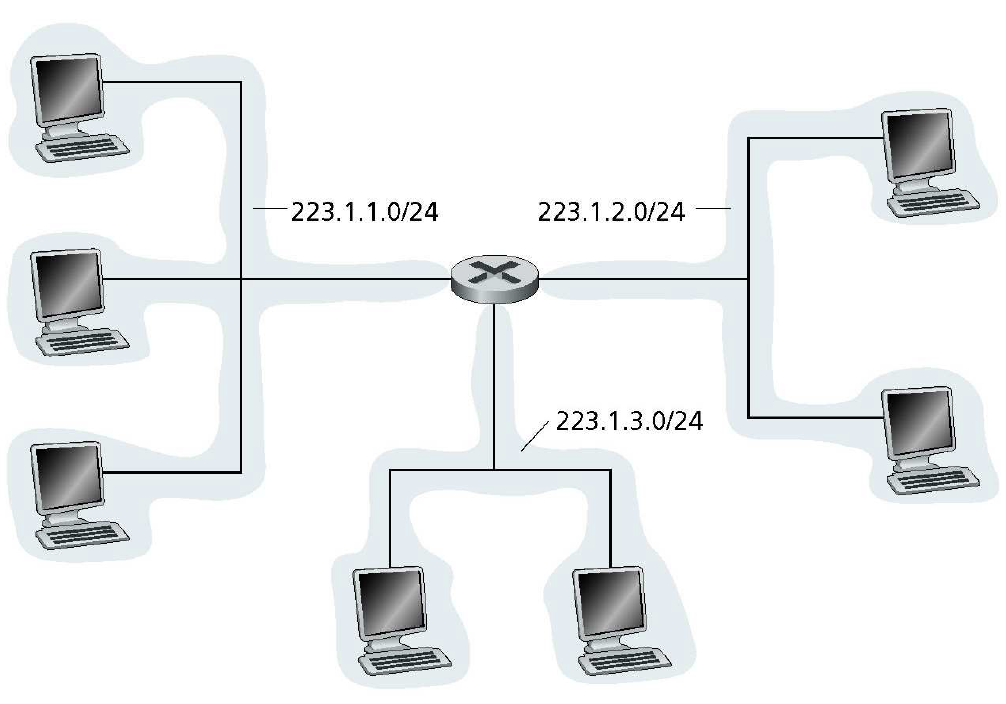
\includegraphics[width=0.5\linewidth]{./images/reteip.png}
\end{figure}

L'interfaccia di rete di un router e i dispositivi a essa collegata (magari tramite uno switch o da un punto di accesso Wireless) costituiscono una sottorete [RFC 950]. Ad esempio, IP assegna ad una sottorete l'indirizzo \verb|223.1.1.0/24|. La notazione \verb|/24| è chiamata maschera di rete, ed indica che i 24 bit più a sinistra dell'indirizzo definiscono l'indirizzo della sottorete. Questo vuol dire che tutti i dispositivi partecipanti a questa rete avranno indirizzo IP nella forma \verb|223.1.1.XXX|\footnote{Con XXX nel range $[2-254]$, escludendo $0$ in quanto \textit{forbidden}, 1 riservato ai router e 255 per il broadcast}.



\subsubsection{Regola generale per individuare sottoreti}
\textit{Per determinare le sottoreti, si sgancino le interfacce da host a router in maniera tale da creare isole di reti isolate delimitate dalle interfacce. Ognuna di queste reti isolate viene detta sottorete.}

\newpage
\subsection{CIDR - Classless InterDomain Routing}
CIDR [RFC 4623] (pronunciato \textit{Cider}) generalizza l'indirizzamento di sottorete nel seguente modo:

\begin{itemize}
	\item L'indirizzo IP è nella forma $a.b.c.d/x$
	\item $x$ indica il numero di bit della prima parte dell'indirizzo.
	\item La prima porzione è detta porzione di rete, o prefisso, dell'indirizzo IP. 
	\item La seconda porzione (di $32-x$ bit) distingue i dispositivi all'interno della stessa rete, o delle ulteriori sottoreti.\\
	\textit{Un esempio? La rete denotata da $a.b.c.d/21$ contiene anche la sottorete denotata da $a.b.c.d/24$, all'interno della stessa organizzazione.}
\end{itemize}

Questo metodo è stato introdotto dopo l'utilizzo del classful addressing, che segue la suddivisione in classi che abbiamo introdotto precedentemente.\\ Detto ciò, la suddivisione meno rigida del CIDR ha permesso alle aziende di scegliere un valore di $x$ che minimizzi lo spreco di indirizzi IP, ottenendone invece un quantitativo che rispecchi quanto possibile le esigenze del sistema.

\subsubsection{Da una domanda su stack overflow}

\begin{small}
	\begin{verbatim}
		Class based addressing basically divides the total IPv4 range into five classes: 
		Class A through E; Whereas CIDR is based on concept of subnetting.
		
		Your company wants 32 public ip addresses.
		If we assign them a class C address, for example 192.168.2.0, their company 
		reserves all IP addresses in range 192.168.2.1 - 192.168.2.254. 
		
		But they only want 32 ip addresses which means 223 addresses will be wasted.
		This is the constraint of classful addressing. Now if we look at just subnetting, 
		class c ip address has default subnet of 255.255.255.0 so if we divide the range of 
		192.168.2.0 in 6 subnets each containing 32 available ip addresses your problem 
		is solved. 
		
		But, if we take this example to higher level we will require CIDR.
		According to traditional subnetting, we can not combine the addresses from the networks 
		192.168.2.0 and 192.168.3.0 because the netmask for class C addresses is 255.255.255.0. 
		However, using CIDR notation, we can combine these blocks by referencing this chunk as 
		192.168.2.0/23.
		
		This specifies that there are 23 bits used for the network portion that we are 
		referring to. 
		With this, the 24th bit can be either 0 or 1 and it will still match, because the 
		network block only cares about the first 23 digits.
		
		CIDR allows more control over addressing continuous blocks of IP addresses. 
		This is much more useful than the subnetting we talked about originally.
	\end{verbatim}
\end{small}
\subsubsection{IP broadcast}
\verb|255.255.255.255|. Quando un host emette un datagramma con tale IP destinazione, il messaggio viene consegnato a tutti gli host sulla stessa sottorete.



\newpage

\subsection{Come vengono usate le maschere di rete}
La maschera di rete, indicata in notazione CIDR con $/x$ indica che i primi $x$ bit a sinistra indicano la (sotto)rete. Nella maschera di rete, i primi $x$ bit a sinistra saranno 1, gli altri $32-x$ a 0. Alcuni esempi di maschere di rete:
\begin{itemize}
	\item Con $/19$ la maschera sarà: \verb|255.255.224.0| - \verb|11111111111111111110000000000000|
	\item Con $/24$ la maschera sarà: \verb|255.255.255.0| - \verb|11111111111111111111111100000000|
	\item Con $/16$ la maschera sarà: \verb|255.255.0.0| - \verb|11111111111111110000000000000000|
\end{itemize}
\begin{figure}[htp]
	\centering
	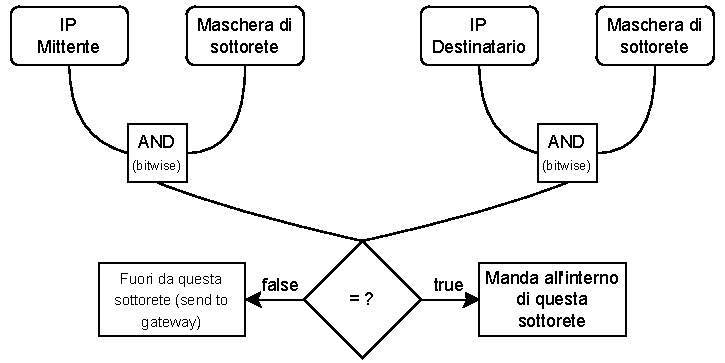
\includegraphics[width=1\linewidth]{./images/netmask.pdf}
\end{figure}
La maschera di rete può essere usata per estrapolare e confrontare l'indirizzo della sottorete di appartenenza di due host.

\newpage

\section{Elementi del livello di collegamento e ARP}
Studiando il livello di collegamento, scopriremo che gli host e i router hanno un indirizzo sia a livello di rete (IP) che a livello di collegamento (indirizzo MAC).
Il protocollo ARP (\textit{address resolution protocol}) permette  ai nodi l'associazione indirizzo IP $\to$ indirizzo MAC.

\subsection{Cos'è un indirizzo MAC?}
Un indirizzo \textit{Media Access Control} è un codice a 6 byte che identifica univocamente una scheda di rete. Gli indirizzi MAC sono univoci: la IEEE si occupa di distribuire proprio questi indirizzi MAC alle varie aziende. I primi 3 byte sono stabiliti dall'IEEE, (viene scelta quindi una combinazione di bit su $2^{24}$). Gli ultimi tre vengono dati univocamente ad ogni dispositivo prodotto dall'azienda stessa (sempre $2^{24}=16.777.216$).

\subsection{Il protocollo ARP}
Sta per \textit{Address Resolution Protocol} [RFC 826], e traduce gli indirizzi IP in MAC address. Traduce gli indirizzi IP di dispositivi situati nella stessa sottorete. Convenzionalmente, gli indirizzi IP sono scritti in decimale, gli indirizzi MAC in esadecimale.

\subsubsection{Come funziona?}
Ogni nodo contiene una tabella ARP cui record contengono tre valori: \\ \verb|Indirizzo IP - Indirizzo MAC - Time To Live|.\\
Il time-to-live specifica tra quanto tempo quel determinato record dovrà essere eliminato dalla tabella. Un tempo tipico sono 20 minuti.


\subsubsection{Caso 1 - Invio sulla stessa (sotto)rete}

\begin{enumerate}
	\item Se un datagramma deve essere mandato da un host $A$ a un host $B$ nella stessa sottorete, $A$ dovrà conoscere l'indirizzo MAC di quel dispositivo. 
	
	\item Se l'indirizzo MAC è già presente nella ARP del nodo, questo manderà il datagramma senza ulteriori passaggi.
	
	\item Altrimenti, manderà una cosidetta "richiesta ARP" contenuta in un pacchetto ARP mandato all'indirizzo broadcast della rete \verb|FF-FF-FF-FF-FF-FF|.
	
	\item Il pacchetto conterrà sia l'indirizzo IP e MAC del mittente, che l'indirizzo IP del destinatario.
	
	\item La richiesta broadcast verrà mandata a tutte le schede di rete della sottorete. La risposta ARP verrà mandata in modalità non-broadcast dal dispositivo con indirizzo IP uguale a quello della richiesta, verso il richiedente. La risposta ARP conterrà al suo interno l'indirizzo MAC del ricevente della richiesta, e la tabella ARP verrà aggiornata.
\end{enumerate}

\newpage

\subsubsection{Caso 2 - Invio su (sotto)rete diversa}
Alice desidera mandare un messaggio a Bob, collegato ad una sottorete diversa.
\begin{enumerate}
	\item Alice manda il datagramma alla sua scheda di rete. Dovrà indicare l'indirizzo MAC\\ dell'interfaccia del router a cui è collegato. Se l'indirizzo MAC è già presente nella tabella ARP di Alice, questo manderà il datagramma al router.
	
	\item Altrimenti, userà il protocollo ARP per ottenere l'indirizzo MAC. Manderà una richiesta ARP all'indirizzo broadcast della rete \verb|FF-FF-FF-FF-FF-FF|, contenente l'indirizzo IP del router.\\
	Il router, riconoscendo il proprio indirizzo, risponderà con una ARP reply condividendo ad Alice il proprio indirizzo MAC. Alice memorizzerà il nuovo indirizzo MAC appena scoperto nella propria tabella ARP, e manda il proprio frame.
	
	\begin{figure}[htp]
		\centering
		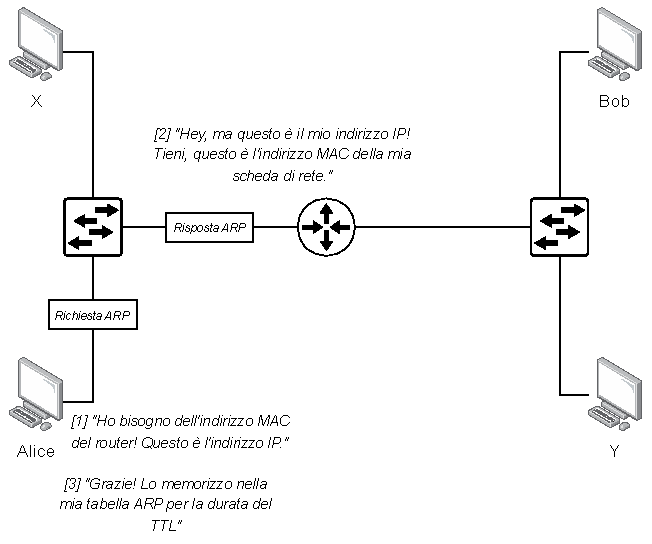
\includegraphics[width=0.75\linewidth]{./images/1-fuoridallasottorete.drawio.pdf}
	\end{figure}
	
	
	\item Il router confronta l'IP del pacchetto con la propria tabella di inoltro. Sa che il pacchetto deve essere inoltrato all'interfaccia 2, ma non conosce l'indirizzo MAC del destinatario Bob.
	
	\begin{figure}[htp]
		\centering
		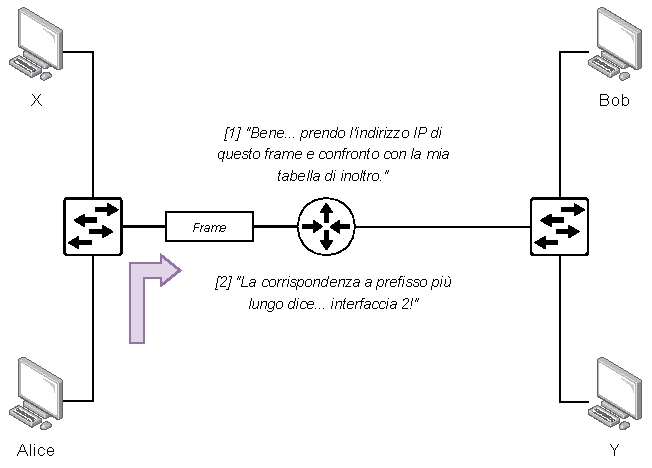
\includegraphics[width=0.75\linewidth]{./images/2-fuoridallasottorete.drawio.pdf}
	\end{figure}
	
	\newpage
	
	\item Il router manda la richiesta ARP, lo switch la manda in broadcast a tutti i dispositivi connessi. Bob riconosce l'indirizzo IP della richiesta ARP, e manda una risposta ARP. Il router riceverà l'indirizzo MAC di Bob, lo conserverà nella propria ARP table assieme al suo IP.
	\begin{figure}[htp]
		\centering
		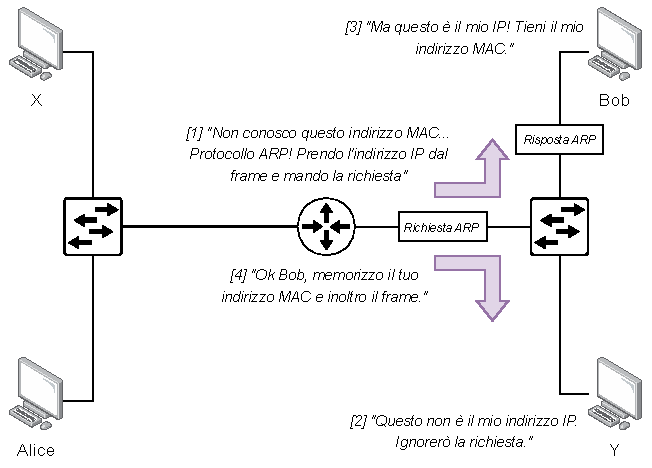
\includegraphics[width=0.75\linewidth]{./images/3-fuoridallasottorete.drawio.pdf}
	\end{figure}
	
	\item Il router avrà tutto il necessario per inoltrare il pacchetto a Bob, ed è ciò che farà.
	\begin{figure}[htp]
		\centering
		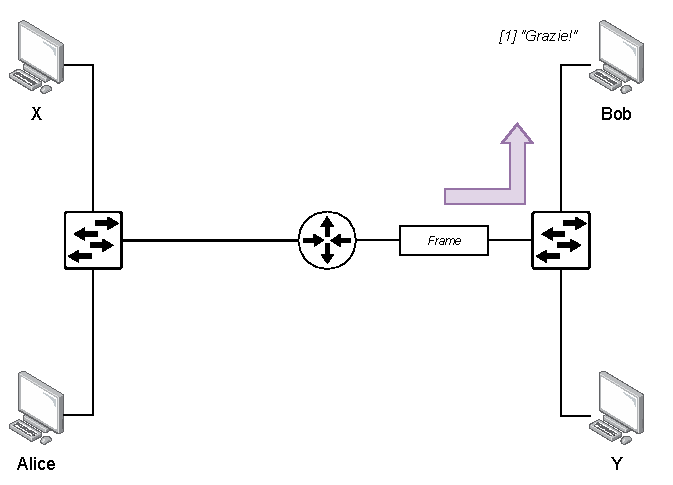
\includegraphics[width=0.75\linewidth]{./images/4-fuoridallasottorete.drawio.pdf}
	\end{figure}
	
\end{enumerate}
Notiamo che, dopo aver ottenuto tutti gli indirizzi necessari, tramite protocollo ARP, per tutta la durata delle \textit{entries} nella tabella ARP, l'inoltro sarà presumibilmente molto più veloce.

\newpage

\section{Ottenere gli indirizzi IP}
Per ottenere un blocco di indirizzi IP da usare in una sottorete, bisogna rivolgersi a Internet Service Provider (ISP). Quest'ultimo attinge da un suo blocco di indirizzi IP già allocati, e ne riserva un numero inferiore per l'ente richiedente. La dimensione della maschera di rete stabilisce la dimensione del blocco allocato.\\
L'ente che ha acquisito gli indirizzi potrà gestirseli autonomamente, costruendo le proprie sottoreti. Ogni ISP richiede uno o più blocchi di indirizzi IP all'ICANN (Internet Corporation for Assigned Names and Numbers). L'Address Support Organization si occupa dell'allocazione e della gestione degli indirizzi all'interno delle rispettive regioni, e quindi dei RIR.

\newpage
\section{DHCP - Dynamic Host Configuration Protocol}
Ottenuto un blocco di indirizzi, li si può assegnare alle interfacce dei router e degli host della propria struttura. La configurazione può avvenire manualmente, o sfruttando il \textbf{Dynamic Host Configuration Protocol} (DHCP) [RFC 2131]. Dipendentemente dalla configurazione del DHCP, gli host possono ricevere indirizzi IP persistenti e uguali a ogni accesso, o uno temporaneo.

\begin{figure}[htp]
	\centering
	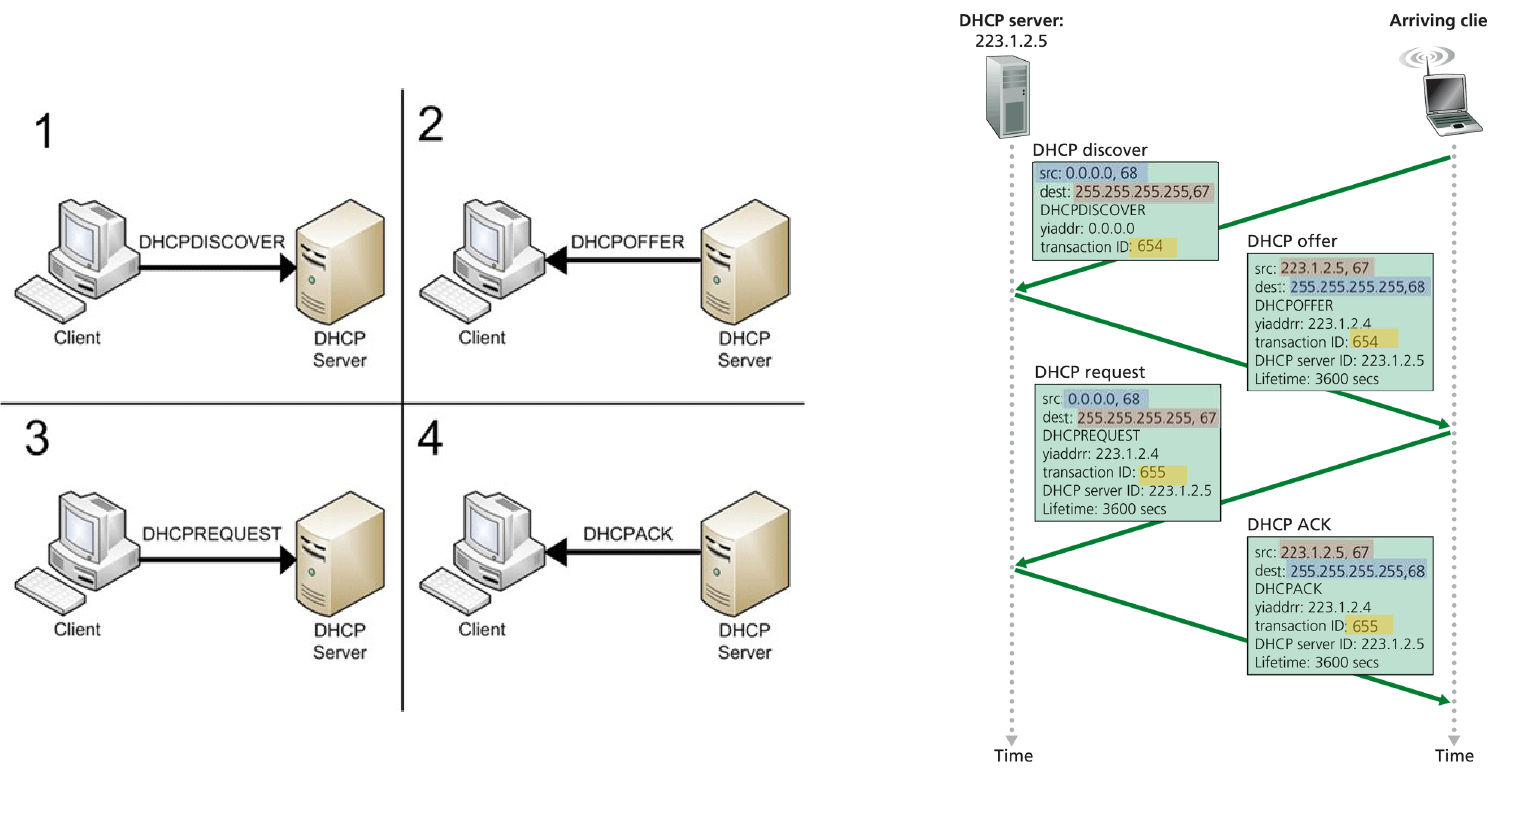
\includegraphics[width=1\linewidth]{./images/dhcp.png}
\end{figure}

\subsection{DHCP - Un protocollo plug-and-play}
Sarebbe impensabile gestire una rete (ad esempio) di un'università o di una scuola: impostare manualmente ogni dispositivo in una struttura con un alto via-vai rappresenterebbe sicuramente una criticità. DHCP imposta automaticamente un indirizzo IP per dispositivi della stessa sotto-rete.

\subsection{Come funziona DHCP}
È un protocollo client-server, in cui i client sono degli host appena connessi alla rete, richiedenti un nuovo indirizzo IP. Il server in ascolto è proprio un server DHCP, che può essere presente nella sottorete, o un relay DHCP all'interno del router che delega il lavoro ad un DHCP esterno.\\
La configurazione di un nuovo host avviene in 4 passaggi:

\begin{enumerate}
	\item \textbf{Individuazione del server DHCP.}\\
	\verb|SOURCE: IP 0.0.0.0, PORT 68  -  DESTINATION: IP 255.255.255.255 PORT: 67|.\\
	Il client manda un messaggio di tipo \textbf{DHCP discover}.
	Il messaggio è incapsulato in un \\pacchetto UDP mandato alla porta 67, e in un datagramma IP mandato in broadcasting, e quindi all'IP \verb|255.255.255.255|. Questo messaggio proviene dalla porta 68, e ha come IP del mittente l'ip \verb|0.0.0.0|.
	
	\item \textbf{Offerta del server DHCP.}\\
	\verb|SOURCE: IP dhcp_server_ip, PORT 67  -  DESTINATION: IP 255.255.255.255 PORT: 68|.\\
	Ricevuto il discover, uno o più server DHCP manderanno un broadcast \textbf{DHCP offer}.\\
	Se il client riceve più offerte, potrà scegliere quello che più preferisce. 
	L'offerta DHCP contiene l'indirizzo IP offerto, l'id transazione, l'IP del server THCP e il \textbf{lifetime} dell'IP offerto.
	
	\item \textbf{Richiesta DHCP.}\\
	\verb|SOURCE: IP 0.0.0.0, PORT 68  -  DESTINATION: IP 255.255.255.255 PORT: 67|.\\
	Il client risponde con un messaggio \textbf{DHCP request}, che riporta i parametri di configurazione.
	
	\item \textbf{Conferma DHCP.}\\
	\verb|SOURCE: IP dhcp_server_ip, PORT 67  -  DESTINATION: IP 255.255.255.255 PORT: 68|.\\
	Conferma da parte del server dei parametri richiesti con un \textbf{DHCP ACK}.
\end{enumerate}

\newpage


\newpage

\section{NAT - Network Address Translation}
\subsection{Problema da risolvere}
Ogni dispositivo ha bisogno di un indirizzo IP. Ne consegue che, al crescere del numero dei dispositivi da connettere ad una rete LAN, (apparentemente) sarà necessario avere un blocco di indirizzi di dimensione crescente. Questo approccio porta problemi: cosa si fa se necessito dall'ISP degli IP contigui che sono stati già allocati? 

\subsection{Soluzione, NAT!}
Nella rete si usa un router abilitato al NAT. A tutti i dispositivi della rete, verranno assegnati indirizzi di spazi di indirizzamento dedicati alle reti private, come lo spazio \verb|10.0.0.0/8|. Nell'esempio in questione, le nostre interfacce di rete avranno indirizzi dello spazio \verb|10.0.0.0/24|. Questi indirizzi non saranno visibili all'esterno, e quindi potranno essere riutilizzati in tutte le possibili reti private separate da router abilitati al NAT.\\
Il NAT ha il compito di tradurre gli indirizzi IP della propria sotto-rete sfruttando una NAT table, in cui i record sono del tipo
\begin{verbatim}
	
\end{verbatim}

\begin{figure}[htp]
	\centering
	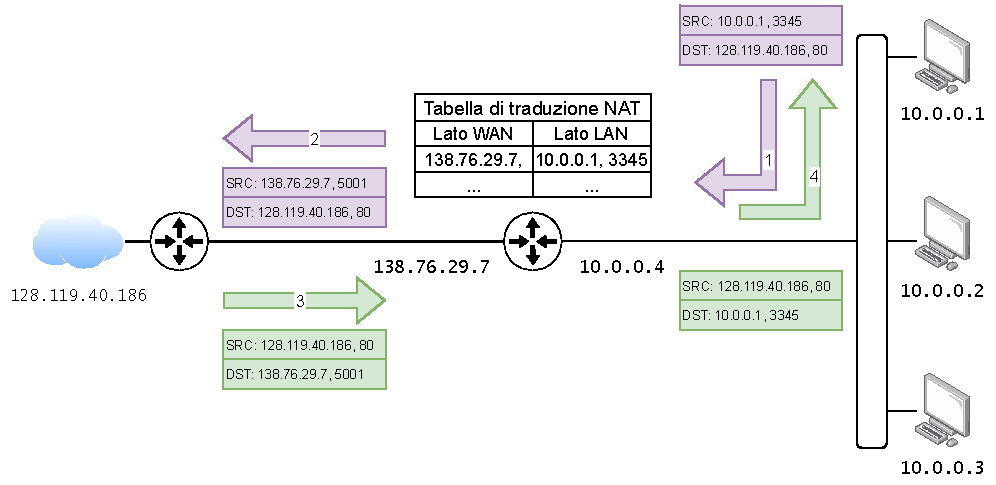
\includegraphics[width=1\linewidth]{./images/NAT.drawio.pdf}
\end{figure}

\begin{enumerate}
	\item Il router riceve i pacchetti da mandare all'esterno. Il NAT controlla se la coppia IP e porta è già presente nella tabella. Se non è presente, il NAT inserisce nella sua tabella un nuovo record, che servirà per le traduzioni. Nel lato LAN l'ip e la porta dell'interfaccia effettiva, nel lato WAN l'IP dell'interfaccia usata dal router lato WAN, e una porta generata casualmente tra quelle non usate dal quell'IP. Il NAT può gestire ben oltre 60.000 connessioni simultane con una sola interfaccia (e indirizzo IP) lato WAN!
	
	\item Il NAT controlla la propria tabella, e sostituisce IP e la porta \verb|SOURCE| del pacchetto, con quelli associati lato WAN. Inoltra regolarmente il pacchetto.
	
	\item Quando riceverà una risposta, i pacchetti arriveranno all'IP e alla porta che il NAT ha precedentemente assegnato.
	
	\item Il NAT stesso si occuperà di tradurre, dal verso opposto, la coppia IP-porta lato WAN, a quella lato LAN, inoltrando regolarmente il pacchetto.
\end{enumerate}
Il NAT non è assolutamente un protocollo perfetto. Implica una violazione del principio end-to-end, a causa della modifica dell'indirizzo IP e del numero di porta. Inoltre, causa problemi con le connessioni P2P e gli applicativi non NAT-friendly.

\newpage

\section{IPv6}
Il protocollo IPv6 nasce dall'esigenza di avere uno spazio di indirizzamento più ampio (tamponare il problema col protocollo NAT non sarebbe stato ottimale e sufficiente a lungo termine), migliorare e semplificare il protocollo IPv4. Imparando dal suo predecessore, è stato possibile creare un protocollo:
\begin{itemize}
	\item Con header più semplici.
	\item Sicuro, tramite un supporto nativo per la sicurezza (IPsec\footnote{IPsec, abbreviazione di IP Security, è uno standard per reti a pacchetto che si prefigge di ottenere connessioni sicure su reti IP. Tale sicurezza viene raggiunta attraverso l'aggiunta di funzionalità di autenticazione, cifratura e controllo di integrità dei pacchetti IP (datagrammi), incluse nell'omonima suite di protocolli e header aggiuntivi.}).
	\item Con Quality of Service migliorata.
	\item Supporto a comunicazione multicast e anycast.
\end{itemize}

\subsection{Parentesi storica}
Nei primi anni '90, si iniziò a progettare il successore di IPv4. Le motivazioni erano chiare: avere 32 bit per ogni indirizzo IP stava diventando limitante, la richiesta di indirizzi IP stava diventando sempre maggiore e meno soddisfacibile. I tecnici della \textbf{Internet Engineering Task Force} (IETF) hanno quindi colto l'occasione per creare un nuovo protocollo, migliore e con un margine di indirizzi IP molto più vasto.

\begin{figure}[htp]
	\centering
	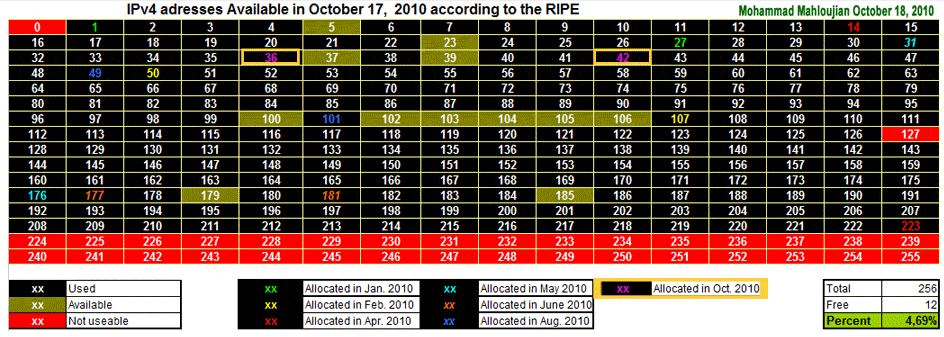
\includegraphics[width=1\linewidth]{./images/ipv4takenaddresses.png}
	\caption{Disponibilità IPv4 del 2010, dal Réseaux IP Européens, ovvero il RIR europeo.}
\end{figure}

\subsection{Funzionalità rimosse}
Nella prossima sezione, andremo a revisionare la struttura dei datagrammi IPv6. Anticipiamo però, quali campi e funzionalità non ritroveremo da IPv4 in quanto rimosse:
\begin{itemize}
	\item \textbf{Frammentazione e riassemblaggio.}\\
	IPv6 \textbf{non consente la frammentazione} e il conseguente \textbf{riassemblaggio nei router intermedi}. Questi passaggi sono \textbf{solo consentiti al mittente e al destinatario}. Quando un router riceve un datagramma IPv6 troppo grande, lo cestina e rimanda al mittente un errore ICMP. Il mittente andrà a frammentare i dati in datagrammi IP più piccoli. La Maximum Transmission Unit minima è 1280 byte, con un consigliato di 1500 byte.
	
	\item \textbf{Checksum dell'header rimosso.}\\
	I protocolli TCP e UDP del livello di trasporto, ed Ethernet, del DLL, implementano già un checksum. Si è quindi preferito \textbf{rimuovere una funzionalità ridondante}.
	
	\item \textbf{TTL - Time To Live.}\\
	Si è deciso di semplificare anche questa funzione, sostituendola con un numero di salti tra router massimo.
	
	\item \textbf{Options.}\\
	Le opzioni aggiuntive per i datagrammi IPv6 sono implementate tramite degli header extra che possono essere aggiunte specificando nel campo "Prossimo header" un numero specifico. Osserveremo dopo questo campo.
\end{itemize}
\newpage

\subsection{Struttura dei datagrammi IPv6}
\begin{figure}[htp]
	\centering
	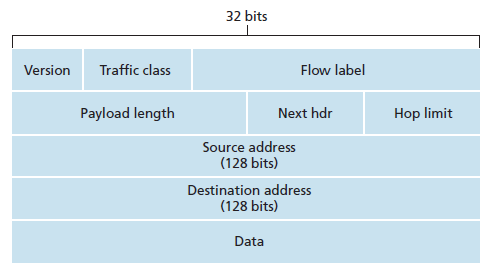
\includegraphics[width=0.75\linewidth]{./images/ipv6structure.png}
\end{figure}

\begin{itemize}
	\item \textbf{Version - Versione.}\\
	Indica la versione di IP usata dal datagramma. 4 bit.
	
	\item \textbf{Traffic Class - Classe di traffico.}\\
	Somiglia al Type of Service di IPv4. Specifica la priorità di un determinato datagramma all'interno di un flusso. VoIP manderà datagrammi di priorità più alta rispetto a SMTP. 8 bit.
	
	\item \textbf{Flow label - Etichetta di flusso.}\\
	Identifica un flusso di datagrammi. 20 bit.
	
	\item \textbf{Payload length - Lunghezza del Payload.}\\
	Interpretato come un unsigned int, indica il numero di byte del datagramma IPv6 a seguire dell'header di dimensione fissa. Il massimo di dati che è possibile trasportare sul payload, è di $2^{16}-1=65,535$. 16 bit. 
	
	\item \textbf{Next header - Prossimo header.}\\
	Specifica il tipo del prossimo header. Questo, può essere l'header del protocollo del livello di trasporto (\verb|TCP: 6, hex 0x06|, \verb|UDP: 17, hex 0x11|), o un header aggiuntivo (\textit{extension header}). Ognuno di questi header aggiuntivi, contiene al suo interno anche il campo \textit{next header}, in modo da poter costruire, su un datagramma, una "catena di header". In questa catena, l'ultimo header aggiuntivo contiene al suo interno il tipo dell'header del livello di trasporto. 8 bit.
	Tra questi header aggiuntivi, abbiamo, ad esempio \verb|Authentication Header (AH): 51| e \\ \verb|Encapsulating Security Payload (ESP): 60|, entrambi meccanismi di \textbf{IPsec}.
	
	\item \textbf{Hop limit - Limite di Hop.}\\
	Un numero che viene decrementato ad ogni inoltro, da parte di router, del datagramma che lo contiene. Quando questo numero diventa 0, viene cestinato. 8 bit.
	
	\item \textbf{Indirizzi.}\\
	Sorgente e destinazione, entrambi a 128 bit.
	
	\item \textbf{Dati.}
\end{itemize}

\newpage

\subsection{Funzionalità di IPv6}
Sintetizziamo in breve gli aspetti \textit{game changer} del protocollo IPv6.
\begin{itemize}
	\item \textbf{Indirizzamento esteso.}\\
	Aumenta la dimensione degli indirizzi. $2^{128}$ indirizzi possibili, praticamente inesauribili. 
	\item \textbf{Unicast, Multicast e Anycast.}\\
	Supporta indizzi unicast, multicast ed anycast. Gli indirizzi multicast e anycast identificano insiemi di interfacce. Mandando un pacchetto a un'indirizzo multicast, questo verrà mandato a tutte le interfacce. Mandando un pacchetto a un'indirizzo anycast, questo verrà all'interfaccia più vicina (o una qualunque).
	\item \textbf{Etichettatura dei flussi.}\\
	Etichettando in un determinato modo i pacchetti di un determinato flusso, diventa possibile dare priorità e offrire delle garanzie di servizio migliori rispetto a determinati protocolli dell'application layer.
	\item \textbf{Rimossa frammentazione ai router intermedi.}
	\item \textbf{Sfoltiti gli header.}
\end{itemize}


\subsection{Sugli indirizzi IPv6}
Per convenzione, i molto più lunghi indirizzi IPv6, rispetto agli IPv4, sono scritti in esadecimale. Otto gruppi da quattro cifre, separati da due punti.

\begin{verbatim}
	esempio di indirizzo IPv6:
	8000:0000:0000:000:0123:4567:89AB:CDEF
	
	o, equivalente:
	8000::123:4567:89AB:CDEF
	
	un indirizzo IPv4 mappato in IPv6:
	::151.97.1.1
	
	indirizzo di loopback:
	::1
	
	non specificato:
	::
\end{verbatim}

\subsubsection{Assegnazione indirizzi IPv6}
\begin{footnotesize}
	\begin{figure}[htp]
		\centering
		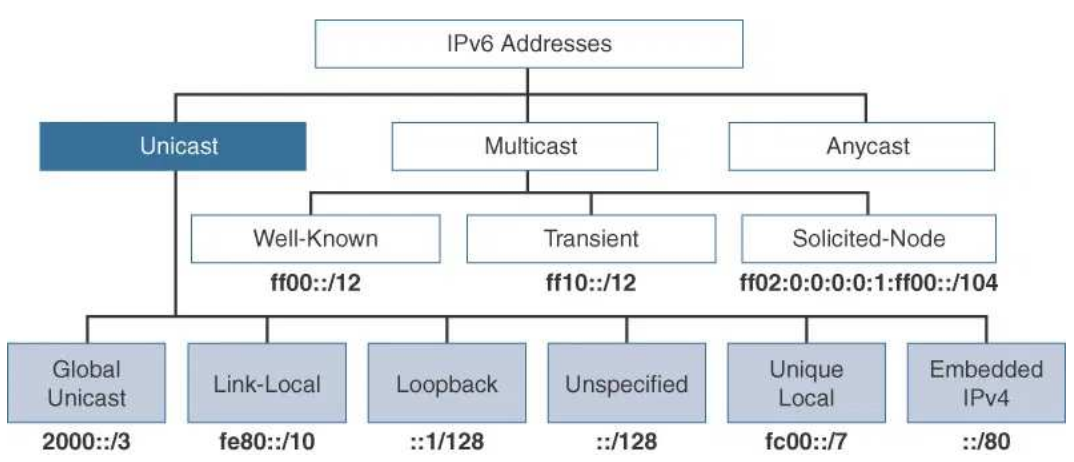
\includegraphics[width=0.85\linewidth]{./images/ipv6indirizzamento.png}
	\end{figure}
\end{footnotesize}
\newpage

\subsection{EUI-64 - Extended Unique Identifier}

L'assegnamento di un indirizzo IPv6 ad un'interfaccia di rete avviene tramite DHPC. Tuttavia, prima dell'assegnamento\footnote{Invece di usare l'indirizzo 0.0.0.0}, questo può essere automaticamente derivato dal suo MAC address a 48 bit, seguendo il metodo \textbf{EUI-64}. \textbf{Utile in configurazioni senza DHCPv6}.

\begin{enumerate}
	\item Si prende l'indirizzo MAC.
	\item Si divide in due metà (24 bit ciascuna).
	\item Si inserisce in mezzo \verb|FF:FE|. (In Windows, vengono inserite delle cifre casuali).
	\item Si cambia il settimo bit (universal/local) del primo byte in 1 se è un indirizzo localmente amministrato, a 0 se è globalmente unico.
\end{enumerate}

Questi indirizzi funzionano solo all'interno di una LAN.
\subsection{Neighbour Discovery Protocol (il nuovo arp!)}
È il protocollo simil-ARP di IPv6. Migliore di ARP, usa ICMPv6, e sfrutta due tipi di messaggi:

\begin{itemize}
	\item \textbf{Neighbour Solicitation (NS).}\\
	Equivalente di un ARP request. Richiede l'indirizzo MAC di un dispositivo con un determinato indirizzo IPv6.
	\item \textbf{Neighbour Advertisement (NA).}\\
	È l'equivalente dell'ARP reply. Può essere anche spontanea senza previa NS, per avvisare i dispositivi di cambiamenti del MAC address.
\end{itemize}
Questo protocollo permette anche di \textbf{autoconfigurare gli host}, e supporta \textbf{Router Advertisement}.

\subsection{IPv6 over Ethernet}
Come IPv4, anche i datagrammi IPv6 viaggiano dentro frame Ethernet. Il pacchetto Ethernet, in questo caso, conterrà nel campo Ethertype il codice \verb|0x86DD|, e non \verb|0x0800| di IPv4.


\subsection{Da IPv4 a IPv6}
L'argomento transizione da IPv4 a IPv6 è un argomento \textbf{delicato}: l'infrastruttura di Internet è stata costruita su IPv4, ma in pochi avrebbero potuto prevedere un tale successo. IPv6 è il sostituto definitivo di IPv4, ma il processo di transizione sarà lento e durerà ancora anni. Non potrà mai essere rapido com'è stato, ad esempio, quello dal protocollo NCP (protocollo di trasporto risalente alla rete ARPANET) a quello TCP.

\subsubsection{Dual Stack}
I dispositivi (host o router) supportano entrambi i protocolli, IPv4 e IPv6. Quello scelto dalle applicazioni dipenderà dal tipo di connessione (con una preferenza verso IPv6).
Questo aumenta la complessità di gestione del nodo, a causa del doppio IP, ma è la soluzione più semplice e stabile.

\subsubsection{Tunneling}
Se i due end-point di una comunicazione supportano IPv6, ma parte della rete che devono attraversare i messaggi no, ciò che si farà, sarà incapsulare l'intero datagramma IPv6 in datagrammi IPv4 prima di essere inoltrato all'interno della rete che supporta IPv4.

\newpage
\section{ICMP - Internet Control Message Protocol}
È un protocollo usato per la trasmissione di informazioni di controllo nella rete. Viene in IP ed è utilizzato per strumenti vari, tra cui \verb!ping! e \verb|traceroute|.
ICMP esiste sia per IPv4 che per IPv6, e in IPv6 trova importante applicazione per i messaggi del \textbf{Neighbor Discovery Protocol}. ICMP include i campi:
\begin{itemize}
	\item \textbf{Tipo.}\\
	Specifica il formato dei messaggi. 8 bit.
	\item \textbf{Codice.}\\
	Identifica il messaggio. 8 bit.
	\item \textbf{Checksum.}\\
	16 bit.
	\item \textbf{Dati.}\\
	La lunghezza di questo campo cambia in base al campo "tipo" e "codice".
\end{itemize}

\section{Firewall}
Sono delle\textbf{ strutture software, hardware o ibride} cui compito è \textbf{bloccare} e/o \textbf{filtrare il traffico malevolo}, in base ai valori relativi ai campi degli header, o effettuano un \textbf{reindirizzamento} per un'ulteriore elaborazione. \textbf{Gestire tutto ciò che costituisce una minaccia per la sicurezza}, e che passa attraverso la rete,\textbf{ è il compito principale dei firewall}, e per adempiere a questo scopo, sono definite delle regole di filtraggio intelligenti, basate su:
\begin{itemize}
	\item Indirizzi IP e porte di origine e destinazione.
	\item Protocolli (TCP, UDP, ICMP...).
	\item Stato della connessione.
	\item \textbf{Contenuto del pacchetto}, in firewall con ispezione profonda.
\end{itemize}

I firewall posso operare a livello di rete, di trasporto e/o al livello applicativo, a seconda delle esigenze di controllo.

\subsection{DMZ - Demilitarized Zone}
Tra una rete locale e una WAN, solitamente, si crea una terza sottorete, chiamata \textbf{Demilitarized Zone}, o \textbf{DMZ}. Questa zona contiene sistemi isolati dalla rete interna, ma raggiungibili dall'esterno, una sorta di \textit{facade} per l'esterno. È qui che i firewall possono:

\begin{itemize}
	\item \textbf{Allow}, far passare un pacchetto.
	\item \textbf{Deny}, bloccare e rispedire un pacchetto al mittente.
	\item \textbf{Drop}, bloccare un pacchetto senza notificarne il mittente. Permette di risparmiare banda. 
\end{itemize}

Un firewall può implementare il NAT, per mascherare gli IP interni alla rete esterna. 

\chapter{Network Layer - Piano di controllo}

\section{Algoritmi di Instradamento (routing)}
Lo scopo di questi algoritmi è \textbf{determinare i migliori cammini} da usare dalle sorgenti ai destinatari. Il miglior cammino è valutato rispetto a vari fattori, che riprendono ciò che abbiamo affrontato nello studio dei problemi di ottimizzazione sui grafi, nella materia Algoritmi e Laboratorio. \href{https://github.com/BoredDam/Algoritmi}{Vedi il mio GitHub per approfondimenti}.

\begin{itemize}
	\item \textit{Shortest path}, o \textit{shortest unweighted path}.\\
	Il cammino, da nodo $A$ a nodo $B$ che passa attraverso il \textbf{minor numero di nodi}.
	
	\item \textit{Shortest weighted path}, o \textit{least-cost path}.\\
	Il cammino $p= \langle (v_1, v_2), (v_2, v_3) \dots, (v_{n-1},v_n) \rangle$ tale che $A=v_1$, $B = v_n$ e 
	$$
	\min \sum_{i=1}^n c(v_{i-1}, v_i)
	$$
	ovvero, tale che la \textbf{somma dei pesi} (o costi) del cammino da $A$ a $B$ sia \textbf{minima}.
\end{itemize}

Nonostante ciò, esistono molti altri fattori da \textbf{tenere in considerazione}, come \textbf{policy} di inoltro.

\subsection{Centralizzati, non centralizzati}
\begin{itemize}
	\item Un \textbf{algoritmo di instradamento centralizzato}, calcola il percorso migliore avendo una\\ conoscenza globale della rete. Ciò implica l'esistenza di un modo per conoscere i costi e la topologia relativi ad una rete. Il calcolo dei percorsi potrà poi essere effettuato da una struttura centralizzata e condiviso ai router, o replicato in ogni router.\\
	Un esempio di algoritmo a informazioni globali (centralizzato), è \textbf{l'algoritmo link-state}.
	
	\item Un \textbf{algoritmo di instradamento decentralizzato}, effettua lo stesso calcolo in maniera distribuita e iterativa. Nessun nodo possiede informazioni di tipo globale relative alla rete, ma solo quelle relative ai collegamenti adiacenti. Lo scambio di informazioni permette gradualmente di valutare il percorso a distanza minima. L'algoritmo decentralizzato che tratteremo sfrutta un vettore, chiamato \textbf{vettore delle distanze}, presente in ogni router, e che contiene al suo interno le stime relative alla lunghezza dei cammini minimi. È detto algoritmo \textbf{distance-vector}.
\end{itemize}

\subsection{Algoritmi statici e dinamici}
\begin{itemize}
	\item Negli \textbf{algoritmi di instradamento statici}, raramente i percorsi stabiliti cambiano. Solitamente ciò avviene sotto intervento umano.
	\item Negli \textbf{algoritmi di instradamento dinamici}, gli instradamenti variano in funzione di fattori quali volume del traffico, topologia della rete. L'algoritmo viene eseguito periodicamente o in funzione di variazioni nella topologia o di costi relativi ai collegamenti.
\end{itemize}
\newpage

\subsection{Algoritmi sensibili o insensibili al carico}
\begin{itemize}
	\item Gli \textbf{algoritmi sensibili al carico} usano il tasso di congestione dei collegamenti come criterio per valutarne il costo. Rispondono meglio ai cambiamenti della rete, ma sono molto sensibili a instradamento in loop e oscillazione dei percorsi.
	
	\item Gli \textbf{algoritmi insensibili al carico} non valutano gli stessi fattori.
\end{itemize}


Un'intuizione iniziale potrebbe farci preferire i primi ai secondi. Tuttavia, il costo di un collegamento calcolato in un momento di congestione, non esprime quello che dovrebbe essere il suo costo in condizioni normali. La congestione di rete potrebbe non durare abbastanza per rendere valida la scelta di un cammino migliore in quell'istante di tempo. Per Internet, si è preferito sfruttare algoritmi di instradamento insensibili al carico.

\subsubsection{Problema delle oscillazioni}
Negli algoritmi sensibili al carico appena accennati, si rischia lo scenario delle \textbf{oscillazioni dei percorsi}. Avviene quando il costo del collegamento è \textbf{pari al traffico trasportato}.

\begin{figure}[htp]
	\centering
	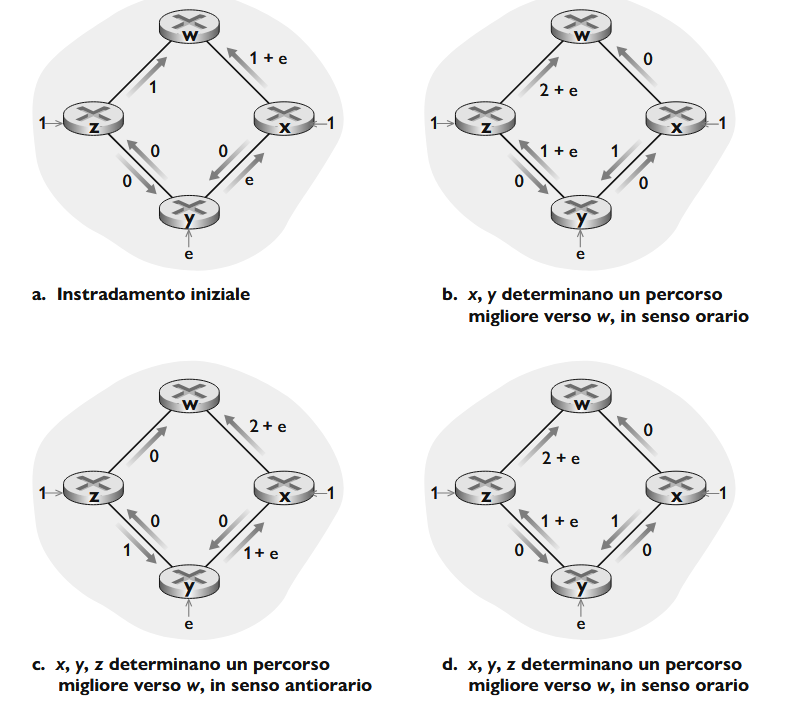
\includegraphics[width=0.75\linewidth]{./images/oscillazione dei percorsi.png}
\end{figure}

Questo scenario, causa cicli di ricalcolo continui che compromettono la stabilità dell'instradamento. La soluzione generale, consiste nell'\textbf{evitare che tutti i router eseguano l'algoritmo di routing allo stesso istante}.
\newpage

\section{Instradamento link-state}
Un \textbf{algoritmo di instradamento centralizzato}, calcola il percorso migliore avendo una conoscenza globale della rete.

\subsection{Flooding e Link state broadcast}
Conoscere la topologia e i costi della rete è quindi fondamentale per effettuare tutti i calcoli necessari. Il protocollo \textbf{Open Shortest Path First} (OSPF), sfrutta il \textbf{link-state broadcast}, ovvero l'invio di un particolare tipo di messaggio, chiamato \textbf{link-state advertisement} che viene distribuito nella rete tramite una tecnica chiamata \textbf{flooding}.

\subsubsection{Flooding}
È un protocollo di instradamento usato dai router: questi \textbf{inoltrano un pacchetto} in ingresso \textbf{su tutte le linee ad eccezione di quella da cui proviene}. Viene usato per \textbf{studiare la topologia della rete} e condividere tra i nodi informazioni relative ai \textbf{costi}.

\begin{figure}[htp]
	\centering
	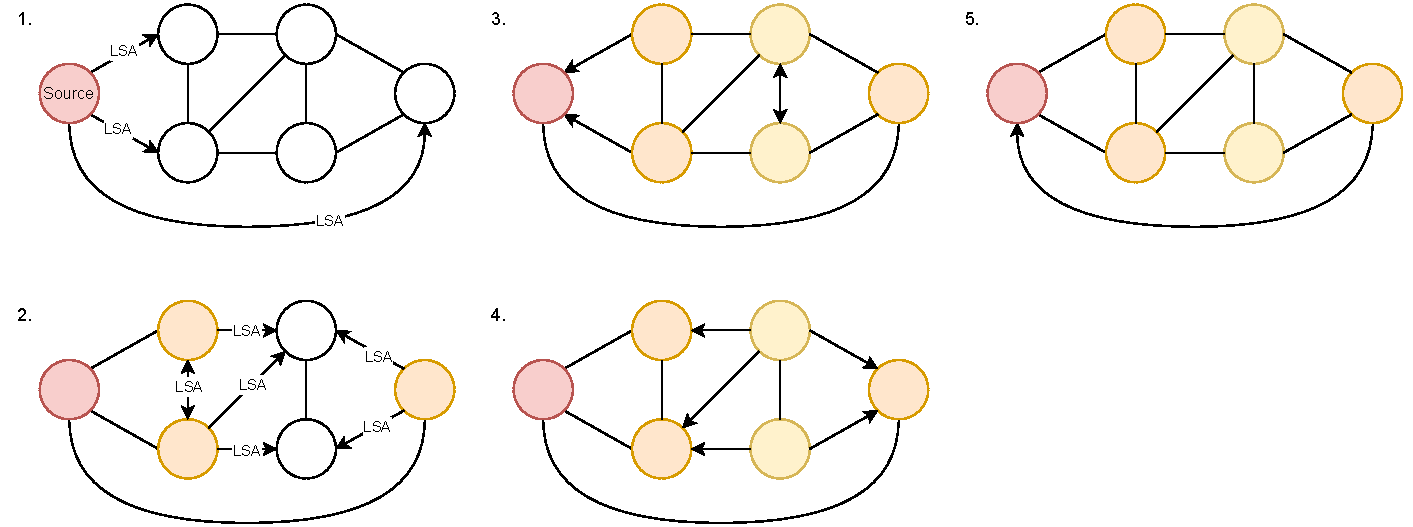
\includegraphics[width=1\linewidth]{./images/flooding.drawio.pdf}
\end{figure}

In reti più complesse e con più cicli, il flooding può creare un numero enorme di pacchetti duplicati, che potrebbero saturare la rete. È quindi consigliato introdurre dei meccanismi che controllino il flooding, come i seguenti:
\begin{itemize}
	\item ID per pacchetto, per evitare i duplicati.
	\item Impostare un limite di hop.
	\item Rimuovere i cicli dal grafo della rete.
	\item Inoltrare i messaggi solo lungo uno spanning tree.
\end{itemize}

\newpage

\subsection{Alcune convenzioni}
\begin{itemize}
	\item $G$ è il grafo.
	
	\item $G.V$ è l'insieme dei nodi del grafo, $G.E$ l'insieme degli archi. $w$ è una funzione (o una struttura dati contenente il) peso, che stabilisce il costo di un arco che unisce due nodi adiacenti.
	
	\item $d.v$ indica il costo minimo stimata dal nodo sorgente nell'iterazione corrente. Parte sempre da $+\infty$, tranne per il nodo sorgente, per cui $d.s = 0$.
	
	\item $\delta(s,v)$ indica l'effettivo costo del cammino minimo dal nodo sorgente a $v$. Presumibilmente, il nostro obiettivo sarà ottenere $d.v = \delta (s,v) \ \forall v \in G.V$.
	
	\item $p.v$ è il predecessore di $v$ all'interno del cammino di costo minimo dal nodo sorgente $s$.
	
	
\end{itemize}
\subsection{L'algoritmo di Dijkstra}
Dato in input un grafo $G$, un nodo sorgente $s$ e una struttura dati contenenti gli archi e il loro peso $w$, Dijkstra calcola tutti i cammini minimi che partono da $s$, verso ogni nodo $v \in G.V$.\\
Si suddivide in due fasi.

\subsubsection{Inizializzazione}
\begin{enumerate}
	
	\item Si pone $d.v= +\infty$ su tutti i nodi, tranne per il nodo sorgente $s$, per cui $d.s=0$.
	
	\item Si pone come $p.v = null$ per ogni nodo.
	
	\item Si crea un insieme $S = \varnothing$, che conterrà tutti i nodi di cui si conosce il cammino di peso minimo da $s$, inizialmente vuoto. Lo utilizzeremo nel corso dell'algoritmo.
	
	\item Si crea una struttura dati $Q = \varnothing$, di cui parleremo meglio dopo.
	
	\item Si inseriscono tutti i nodi all'interno di $Q$.
\end{enumerate}

\subsubsection{Iterazione}
\begin{enumerate}
	\item A ogni passaggio, estrarre il nodo $u$ con $d.u$ minimo da $Q$.\\
	Alla prima iterazione, il nodo estratto sarà $s$.
	
	\item Inserisci $u$ nell'insieme $S$.
	
	\item Verifica se è possibile ridurre $d.v$ dei nodi $v$ adiacenti ad $u$, passando proprio dal nodo $u$. La verifica si ripete su ogni nodo adiacente ad $u$. 
	
	\item Se l'insieme $S = G.V$, smetti di iterare, altrimenti torna al passo 1 dell'iterazione.
\end{enumerate}
Nota bene: ogni volta che è possibile ridurre $d.v$ passando da $u$, bisogna aggiornare il contenuto di $Q$.


\subsection{Complessità dell'algoritmo}
$Q$ sarà una struttura dati su cui effettuare operazioni di inserimento (all'inizio dell'algoritmo), estrazione del minimo e aggiornamento delle chiavi. Definiamo $Q$ come una \textbf{coda con priorità}. L'implementazione di $Q$ influenzerà la complessità dell'algoritmo.
\begin{itemize}
	\item Con $Q$ implementato con un array semplice, avremo una complessità $O(|V|^2)$.
	\item Con $Q$ implementato con un min-heap, si otterrà una complessità $O(|V|+|E|\log|V|)$.
\end{itemize}



\newpage

\section{Instradamento Distance Vector}
L'algoritmo distance-vector sfrutta l'algoritmo \textbf{Bellman-Ford}, creando un nuovo algoritmo asincrono, che girerà sui singoli nodi della rete. Proprio per questo motivo, introduciamo una notazione $D_x[v]$. $D_x$ è il vettore delle distanze, e $D_x[v]$ è la distanza stimata da $x$ a $v$.

\subsection{Algoritmo}
Su ciascun nodo $x \in G.V$ , girerà il seguente algoritmo:
\subsubsection{Inizializzazione}
\begin{enumerate}
	\item $D_x[x]=0$. Il nodo $x$ dista 0 da se stesso. 
	
	\item $\forall v \in G, \ D_x[y] =w (x,y)$. Chiaramente, se $u$ non è adiacente ad $x$, $D_x[u]= +\infty$
	
	\item Inoltra $D_x$ a tutti i nodi adiacenti.
\end{enumerate}

\subsubsection{Iterazione}
\begin{enumerate}
	\item Aspetta fino a quando non ricevi un vettore delle distanze, o finché non cambia il costo verso un nodo adiacente.
	
	\item Ricevuto il vettore delle distanze da un nodo $D_y$, si andrà a calcolare, per ogni $v \in G.V$, 
	$$
	D_x[v] = \min \{D_x[v], \;D_y[v] + w(x,y)\}
	$$
	ovvero, se esiste, calcolo il cammino di peso inferiore per andare da $x$ a $v$, passando per $y$. Se questa condizione si verifica, e la $D_x[v]$ di qualsiasi nodo $v$ cambia, inoltra al vettore delle distanze a tutti i nodi adiacenti.
	
	\item Ritorna allo step 1 dell'iterazione.
\end{enumerate}
Questo algoritmo è un algoritmo \textbf{asincrono}, che\textbf{ itera un numero indefinito di volte su ogni nodo}, in cui i valori minimi calcolati non cambiano, se non successivamente a cambiamenti della rete. In tal caso, ogni nodo cui vettore delle distanze cambia, inoltrerà quest'ultimo agli adiacenti.

\subsection{Poisoned reverse}
Esistono però delle \textbf{circostanze problematiche}, causate dalla \textbf{visibilità limitata} di ogni nodo rispetto ai costi complessivi \textbf{della rete}, che potrebbero causare \textbf{loop di inoltro di pacchetto}. In tal caso, si può introdurre un meccanismo di \textbf{poisoned reverse}, che permette ad un nodo $x$ di mentire a $y$ in una circostanza del genere:
\begin{enumerate}
	\item $y$: voglio inoltrare un pacchetto a $z$ per arrivare a $x$, perché costa meno.
	\item $z$: voglio inoltrare un pacchetto a $y$ per arrivare a $x$, perché costa meno.
\end{enumerate}
Si può arrivare a questa circostanza quando il peso di un arco non adiacente a $z$, ma adiacente a $y$, varia. In tal caso, $z$ vedrà che $y$ vuole arrivare ad $x$ passando da se stesso, osserva che lui farebbe l'opposto, e allora "mente" a $y$ dandogli un costo fittizio $D_z[x]=+\infty$, interrompendo il loop.

\newpage

\section{Routing in Internet}
Per facilitare il routing in Internet, quest'ultimo è organizzato in \textbf{sistemi autonomi} (AS). Ogni sistema autonomo è trattato come una singola entità amministrativa. 
\begin{itemize}
	\item All'interno di sistema autonomo, tutti i router eseguono lo stesso algoritmo di routing, chiamato \textbf{protocollo di instradamento intra-AS}.
	\item Per l‘instradamento tra AS distinti si usano invece \textbf{protocolli di instradamento inter-AS}.
\end{itemize} 
Questa organizzazione in sistemi autonomi, garantisce una maggiore \textbf{autonomia amministrativa} e migliore \textbf{scalabilità}. Ogni sistema autonomo è identificato da un \textbf{numero di sistema autonomo (ASN)}.

\subsection{RIP - Routing Information Protocol (intra-AS)}
È un protocollo di routing basato sull'algoritmo \textbf{Distance Vector} (Bellman-Ford) per il routing interno ai sistemi autonomi. La sua metrica è il \textbf{numero di hop}, ovvero il numero di router da attraversare per raggiungere una determinata destinazione.
\begin{itemize}
	\item Supporta al più 15 hop. Una destinazione $x$ con $d.x=16 \ \text{hop}$ è irraggiungibile.
	\item I router scambiano informazioni relative alle tabelle di routing ogni 30 secondi.
	\item Un percorso non aggiornato per 180 secondi è marcato come irraggiugibile.
	\item Dopo altri 120 secondi viene rimosso dalla tabella (garbage collection).
\end{itemize}
Sfrutta inoltre due tipi di messaggi:
\begin{itemize}
	\item \verb|REQUEST| per richiedere informazioni di routing ai router vicini.
	\item \verb|RESPONSE| per fornire aggiornamenti sulla propria tabella di routing.
\end{itemize}
\subsubsection{Tabelle di routing RIP}
Contengono:
\begin{itemize}
	\item Indirizzo $x$ di destinazione.
	\item Distanza minima (in hop) verso $x$.
	\item Prossimo hop per arrivare a $x$.
	\item Un timeout.
	\item Un timer per la garbage collection.
\end{itemize}

\subsubsection{Versioni di RIP}
\begin{itemize}
	\item \textbf{RIP v1} supporta solo indirizzamento classful senza subnet. Il campo next hop non è esplicito, e non supporta autenticazione.
	\item \textbf{RIP v2} supporta CIDR, Poison Reverse, autenticazione e next hop esplicito nel messaggio.
	\item \textbf{RIPng} (next generation) per IPv6, basata su RIP v2. Non supporta l'autenticazione.
\end{itemize}

\newpage

\subsection{OSPF - Open Shortest Path First (intra-AS)}
È un protocollo di routing intra-AS di tipo \textbf{Link State} usato soprattutto nei contesti di rete medio-grandi e nei \textbf{backbone degli ISP}. È molto scalabile e robusto. Ogni router OSPF:
\begin{itemize}
	\item Costruisce una \textbf{mappa topologica completa} del sistema autonomo usando il flooding. Costruisce un grafo della rete.
	\item Esegue localmente l'algoritmo di Dijkstra e determina l'albero dei cammini minimi da se stesso.
	\item Mantiene un Link-State Database con informazioni sui collegamenti noti.
	\item Manda aggiornamenti periodici tramite dei Link-State Advertisements, rendendo il protocollo molto robusto.
\end{itemize}

I messaggi sono del tipo:
\begin{itemize}
	\item \verb|HELLO|, trasmissione periodica per Neighbor Discovery.
	\item \verb|Database Description|, per condividere le informazioni link-state tra i vari router
	\item \verb|LS Request|, per richiedere parti specifiche del link-state database di un vicino.
	\item \verb|LS Update|, per effettuare il flooding.
	\item \verb|LS ACK|, dei segnali di ACK relativi al Link-State update.
\end{itemize}

E ogni nodo effettua questi passaggi:
\begin{enumerate}
	\item \textbf{Scoperta dei vicini}, in cui i router scoprono i nodi adiacenti inviando messaggi \verb|HELLO|.
	\item \textbf{Sincronizzazione dei database}, \verb|EXCHANGE|, con scambio e confronto delle informazioni Link-State.
	\item \textbf{Aggiornamento dei database}, \verb|FLOODING|, con messaggi tramite cui i cambiamenti dei cammini minimi sono propagati.
\end{enumerate}

\newpage
\subsection{BGP - Border Gateway Protocol}
È un protocollo di routing \textbf{inter-AS}, e quindi tra sistemi autonomi. È fondamentale per il funzionamento di Internet, tanto quanto IP, in quanto \textbf{è il collante tra tutti i vari AS}.
\begin{itemize}
	\item \textbf{Comunicare la raggiungibilità delle sotto reti}.\\
	Permettendo a ciascun sistema di rendersi visibile rispetto i \textbf{prefissi di rete} che gestisce. È tramite BGP che tutti i router conoscono le sottoreti vicine.
	
	\item \textbf{Determinare i percorsi ottimali verso le sottoreti.}\\
	Un router può apprendere più percorsi verso un \textbf{determinato prefisso} (ovvero una sottorete). La selezione del percorso migliore avviene in base alle politiche del sistema autonomo e alle informazioni di raggiungibilità fornite da BGP.
\end{itemize}

\subsubsection{Funzionamento di BGP}
Lo scambio di informazioni avviene tramite dei messaggi scambiati, per ogni coppia di router comunicante, in una sessione TCP. Tra router dello stesso sistema autonomo, sono dette \textbf{sessioni iBGP}. Altrimenti, si dice \textbf{sessione eBGP}. 
\begin{figure}[htp]
	\centering
	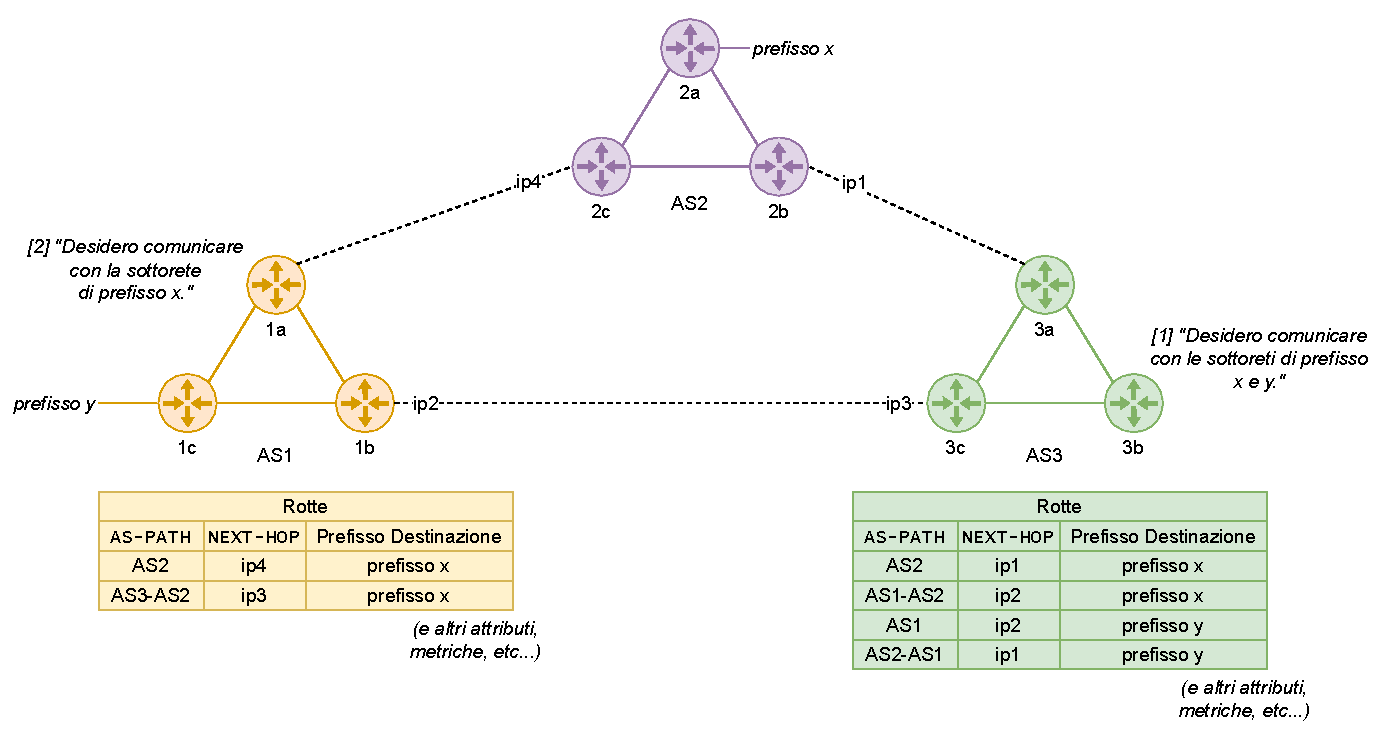
\includegraphics[width=1\linewidth]{./images/BGP.pdf}
\end{figure}

Supponiamo si voglia \textbf{dichiarare la raggiungibilità del prefisso $x$}. L'annuncio di raggiungibilità verrà passato ai nodi adiacenti, che costruiranno una tabella BGP contenente alcuni attributi, tra cui:
\begin{itemize}
	\item \verb|AS-PATH|: indica i sistemi autonomi tramite cui è passato questo annuncio.
	\item \verb|NEXT-HOP|: indica l'IP dell'interfaccia di rete tramite cui "entrare" nel primo sistema autonomo dell'\verb|AS-PATH|.
	\item Il prefisso $x$ da raggiungere.
\end{itemize}

L'insieme prefisso $x$ + attributi è detto \textit{route}, \textbf{rotta}. Valutando ogni \verb|NEXT-HOP| secondo una metrica stabilita, i router possono stabilire il percorso migliore.

\begin{footnotesize}
	\begin{verbatim}
		+------------+------------------------------------------+
		| Code Point |         Metric Type                      |
		+------------+------------------------------------------+
		|     0      | IGP Metric                               |
		|     1      | Min Unidirectional Link Delay [RFC7471]  |
		|     2      | TE Metric [RFC3630]                      |
		|     3      | Hop Count (refer [RFC5440])              |
		|     4      | SID List Length                          |
		|     5      | Loss Rate                                |
		|    6-250   | Unassigned                               |
		|  251-255   | Private Use (not to be assigned by IANA) |
		+------------+------------------------------------------+
		
		Figure 3: Metric Type Code Point  
	\end{verbatim}
\end{footnotesize}

\chapter{Data Link Layer}

\section{Introduzione al livello Data Link}

È il layer che si trova a cavallo tra il mondo logico e quello fisico. Fornisce al livello di rete un \textbf{servizio di trasmissione} per flussi di bit (\textbf{bitstream}).

\subsection{Servizi del Data Link Layer}
\begin{itemize}
	\item \textbf{Data framing.}
	\begin{itemize}
		\item Dal basso verso l'alto, dal fisico al logico\\
		raggruppando simboli/bit del layer fisico in frame e \textbf{trasformando il flusso grezzo} di \textbf{bit} in informazioni strutturate. 
		
		\item Dall'alto verso il basso, dal logico al fisico.\\
		incapsulando i datagrammi del livello di rete in frame contenenti due campi, un campo dati $D$ e i campi d'intestazione.
	\end{itemize}
	\begin{figure}[htp]
		\centering
		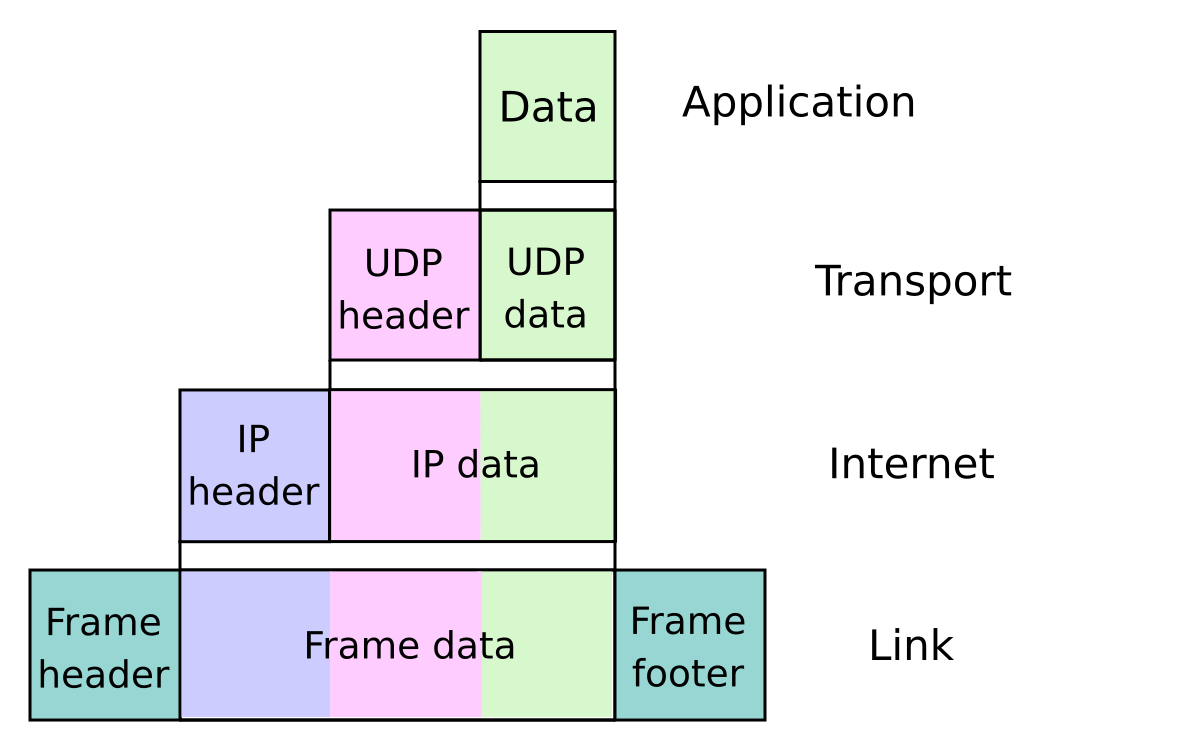
\includegraphics[width=0.5\linewidth]{./images/dataframing.png}
	\end{figure}
	
	\item \textbf{Gestire l'accesso al mezzo fisico}, nel caso di \textbf{canali condivisi}.\\
	I dispositivi, nel DLL, sono identificati tramite indirizzi MAC, dei veri e propri indirizzi fisici. L'accesso al canale condiviso, nel caso dei \textbf{collegamenti broadcast}, dev'essere gestito tramite dei \textbf{protocolli d'accesso multiplo}, per evitare \textbf{collisioni}.
	
	\item Fornire una \textbf{consegna dei dati} \textit{reliable}, \textbf{affidabile}.\\
	Se il mezzo fisico è abbastanza affidabile (fibra, doppino di rame...), non è necessario implementare meccanismi del genere, in quanto ridondanti rispetto a quelli presenti nel livello di trasporto e application. Nel caso di mezzi di trasmissione meno affidabili, come nel caso delle reti wireless, il trasporto reliable è ottenuto tramite meccanismi di ACK/NACK e ritrasmissioni.
	
	\item \textbf{Gestire gli errori} del canale \textbf{di trasmissione} (rilevandoli e, se possibile, correggendoli).\\
	Gli errori possono essere causati da attenuazione del segnale, rumore, interferenze tra campi elettromagnetici o dal mezzo fisico usurato, e sono gestiti tramite checksum, controllo di ridondanza ciclico (CRC), controllo di parità, codici di Hamming o meccanismi simili che conseguono lo stesso scopo.
	
	\item \textbf{Regolare il flusso dati} tra sorgente e destinazione.\\
	I collegamenti possono essere full-duplex o half-duplex, permettendo o non permettendo la trasmissione contemporanea di dati da entrambi i nodi del collegamento. Il pacing di trasmissione deve essere proporzionato a quello di ricezione. I due nodi devono comunicare in maniera opportuna per gestire questa situazione.
\end{itemize}

\subsubsection{Nozione utile - Rumore}
Definiamo come rumore una forma di distorsione (voluta o non voluta) che si presenta all'interno di un segnale elettrico effettivo. Qualsiasi circuito genera rumore, ed è dovuto alla presenza di resistenze (resistenze vere e proprie e resistenza intrinseca dei conduttori elettrici e i materiali usati). Nelle simulazioni dei circuiti elettrici, è possibile inserire un rumore elettrico chiamato \textbf{rumore gaussiano}.

\subsection{Implementazione del DLL - NIC}
In ogni singolo host (device e router) di una rete, è implementato il Data Link Layer. Ciò avviene tramite una combinazione di \textbf{hardware, software e firmware} presente all'interno dei NIC (Network Interface Controller) dei dispositivi di rete. Buona parte del DLL è implementato in hardware, come il protocollo Ethernet nell'adattatore Intel 700, o il protocollo Wi-Fi nel chipset Atheros AR5006. Tuttavia, \textbf{è il software a farsi ponte tra il livello di rete, e il mondo fisico}.

\subsection{Comunicazione tra due Network Interface Controller}
Lato mittente:
\begin{enumerate}
	\item Il datagramma da trasmettere viene incapsulato in un frame del DLL.
	\item I campi d'intestazione del DLL vengono riempiti.
	\item (Se presenti) vengono stabiliti i valori dei bit nei campi per la rilevazione e correzione degli errori.
	\item Il pacchetto viene trasferito.
\end{enumerate}
Dal lato del ricevente:
\begin{enumerate}
	\item Il Network Interface Controller riceve l'intero frame.
	\item (Se presenti) effettua le verifiche relative ai campi di rilevazione e correzione errori.
	\item Estrae il datagramma.
	\item Manda il datagramma al livello di rete+.
\end{enumerate}


\newpage

\section{Data Framing}
Nella trasmissione dei dati, è fondamentale trovare una \textbf{codifica efficace} che permetta di \textbf{interpretare in maniera univoca il segnale elettrico} in stringhe di 0 e 1. A differenza di ciò che si potrebbe pensare, questo problema non è per niente banale. \textbf{Distinguere una sequenza continua di zeri o di 1 da un'interruzione} della trasmissione o da un malfunzionamento \textbf{non è possibile con una codifica a due livelli}.
\begin{figure}[htp]
	\centering
	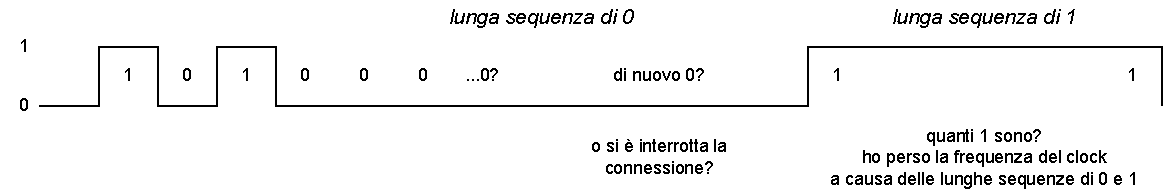
\includegraphics[width=1\linewidth]{./images/2levelencode.pdf}
	\caption{Esempio ipotetico di two-level encoding}
\end{figure}

\subsection{Three-Level Encoding}
Prevede tre livelli di segnale: alto - zero - basso.\\
Segue inoltre delle regole, quali:
\begin{itemize}
	\item Prossimo bit 0.\\
	Nessuna transizione del segnale.
	\item Prossimo bit 1 e livello di segnale $\neq 0$.\\
	Il segnale passa a 0.
	\item Prossimo bit 1 e livello di segnale $=0$.\\
	Il segnale passa ad un livello opposto a quello del più recente segnale diverso da 0.
\end{itemize}

Osserviamo che le transizioni avvengono solo per trasmettere bit $=1$. Inoltre, essendo questa una \textbf{trasmissione asincrona}, una trasmissione di 4 bit$=1$, ossia un ciclo completo, fornirà al receiver un vero e proprio \textbf{clock recovery}, che stabilisce una frequenza di lettura\footnote{Per questo è comune che, in determinati protocolli, la trasmissione sia preceduta da una sequenza di bit chiamata \textbf{preambolo}. Ne parleremo meglio più avanti.} consona, rispetto ai dati in arrivo. 

\begin{figure}[htp]
	\centering
	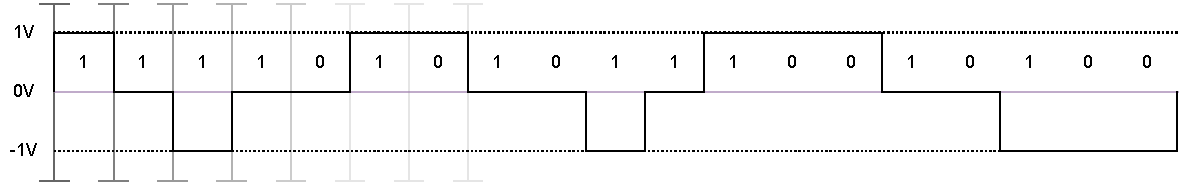
\includegraphics[width=1\linewidth]{./images/3levelencoding.pdf}
\end{figure}

Questo meccanismo di clock permette al receiver di intuire il numero di bit $=0$ da leggere quando, in un quanto di tempo, il segnale rimane ad un certo livello. Chiaramente, lunghe stringhe di zeri possono ancora desincronizzare il receiver, ed è per questo che andremo a parlare (più avanti) di meccanismi che risolvono il problema della \textbf{perdita della sincronizzazione}.


\subsubsection{Esempio di Three-level encoding e Five-level encoding}
\begin{itemize}
	\item La Fast Ethernet (100 BASE TX) utilizza una codifica a tre livelli di segnale: +1V, 0V, -1V. In realtà questi valori non sono statici: sono supportati dei \textbf{range di tollerabilità}.
	\item Specificando più di tre range di voltaggi, e quindi più di tre livelli, diventa possibile trasferire 2 bit alla volta.
	La Gigabit Ethernet (1000 BASE T) utilizza una codifica a cinque livelli: +1V, +0.5V, 0V, -0.5V, -1V. Questa codifica permette di trasmettere in una sola volta i bit \verb|00|, \verb|01|, \verb|10|, \verb|11|, dipendentemente dal livello di segnale.
\end{itemize}

\newpage

\subsection{Codifica a blocchi}
Il three-level encoding è la base per la trasmissione dei dati. Tuttavia, questo meccanismo presenta due criticità:
\begin{itemize}
	\item \textbf{Non è DC-Balanced}. Il livello di tensione medio non è necessariamente mantenuto tendente a 0. Può portare complicazioni di vario tipo.
	\item Se ci sono inoltre lunghe sequenze di zero, si ha un problema di \textbf{perdita di sincronizzazione}.
\end{itemize}
La \textbf{codifica a blocchi} sostituisce blocchi di bit di una determinata dimensione, con blocchi leggermente più grandi ( $4\to5$, $8\to 10$), traducendo le sequenze in maniera tale da garantire un numero minimo di transizioni.

\subsubsection{Codifica 4B5B}
Associa a blocchi di 4 bit, blocchi di 5 bit. Richiede una bandwidth del $25\%$ più capiente. È utilizzata per fast ethernet.

\begin{footnotesize}
	\begin{verbatim}
		Nome    4B           5B          Descrizione
		0       0000         11110       hex data 0
		1       0001         01001       hex data 1
		2       0010         10100       hex data 2
		3       0011         10101       hex data 3
		4       0100         01010       hex data 4
		5       0101         01011       hex data 5
		6       0110         01110       hex data 6
		7       0111         01111       hex data 7
		8       1000         10010       hex data 8
		9       1001         10011       hex data 9
		A       1010         10110       hex data A
		B       1011         10111       hex data B
		C       1100         11010       hex data C
		D       1101         11011       hex data D
		E       1110         11100       hex data E
		F       1111         11101       hex data F
		I       -NONE-       11111       Idle
		J       -NONE-       11000       SSD #1
		K       -NONE-       10001       SSD #2
		T       -NONE-       01101       ESD #1
		R       -NONE-       00111       ESD #2
		H       -NONE-       00100       Halt
	\end{verbatim}
\end{footnotesize}
Questa codifica a blocchi non garantisce DC-balance.
\subsubsection{Codifica 8B10B}

Nella mappatura la sequenza a 8 bit viene divisa in due sottosequenze: una a 5 bit e una a 3 bit. Queste sezioni vengono mappate in modo tale da essere codificate in 6 e 4 bit rispettivamente: concatenate, si ottiene la sequenza di 10 bit. Tra queste sequenze, 12 sono dette \textbf{sequenze di controllo}, come i \textbf{comma}, che permettono al ricevente di allineare in maniera opportuna il flusso di bit. È una codifica \textbf{DC-Balanced}.

\newpage

\subsection{Quantità di informazioni}
Il seguente concetto appartiene alla branca della \textbf{teoria dell'informazione tradizionale}.
Dati $n$ di simboli distinti (in questo caso, livelli di tensione), come \verb|H-M-L| o \\ \verb|HH-HM-HL-MH-MM-ML-LH-LM-LL|, è possibile trasportare un numero di informazioni binarie, quantificate in bit, pari a 
$$
x= \log_2 n
$$


Nel pratico, non potendo esprimere bit parziali, il numero effettivo è dato da

$$
x= \lfloor\log_2 n\rfloor
$$

Con $n=3$ livelli, abbiamo $\lfloor\log_23\rfloor=1$. Con $n=5$ livelli, abbiamo $\lfloor\log_25\rfloor=2$.
Moltiplicando il numero ottenuto, per il numero di step (o simboli) al secondo, otteniamo il \textbf{limite teorico di bitrate}.

$$
\text{Limite teorico bit-rate} = \text{Simboli al secondo} \cdot \log_2 n
$$
\subsubsection{Piccolo approfondimento sulla quantità di informazioni - non è nel programma}
Questa formula è anche detta \textit{Misura di Hartley}, e si tratta di una versione semplificata del concetto di \textbf{entropia informativa di Shannon}, valida solo nel caso di simboli (o eventi) \textbf{equiprobabili}.
\newpage

\section{Gestione degli errori}

\begin{itemize}
	\item L'\textbf{error detection} consiste nell'individuare errori di trasmissione in un frame. Tuttavia non effettua correzione.
	
	\item La \textbf{correzione} permette di individuare errori di trasmissione, ed effettuare correzioni (di dimensioni limitate).
\end{itemize}
Entrambi i metodi sono basati sull'analisi di informazioni ridondanti, per individuare anomalie \\nell'informazione.

\subsection{Ridondanza: elemento di base per l'error detection}
Immaginiamo di voler trasmettere dei dati anagrafici all'interno di un generico pacchetto. Aggiungere allo stesso pacchetto un codice fiscale, mi fornisce delle informazioni sì ridondanti, ma che mi permettono di individuare possibili errori di trasmissione successivamente alla comunicazione.

\subsection{Error Detection}
Un datagramma inoltrato attraverso un mezzo-fisico che ammette errori, contiene al suo interno una sequenza di bit $D$ e un $EDC$ (Error Detection and Correction bits). L'EDC può essere un qualsiasi tipo di controllo, CRC, checksum, controllo di parità.


\begin{figure}[htp]
	\centering
	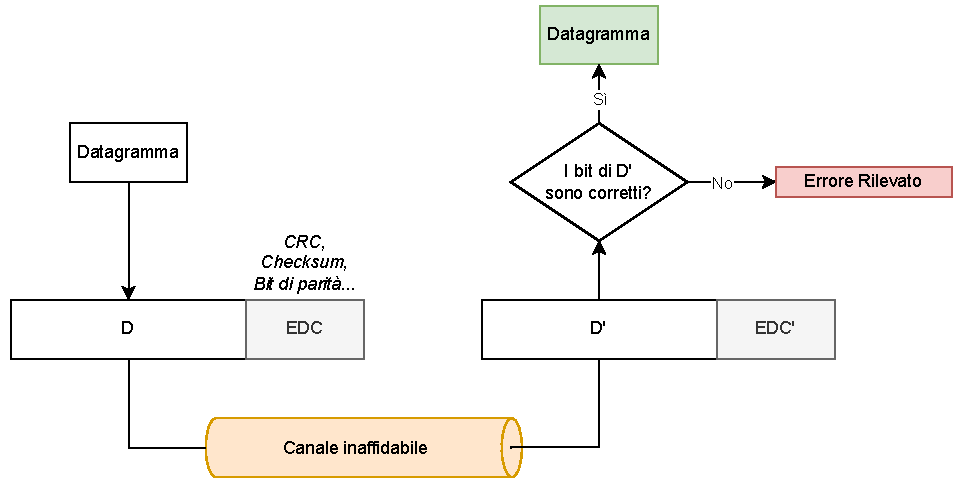
\includegraphics[width=1\linewidth]{./images/edcd.drawio.pdf}
\end{figure}

\newpage


\subsection{Parity check}
Consiste in un bit che specifica se il numero di bit $=1$ è pari o dispari. Può essere un controllo parità a uno o due dimensioni.

\subsubsection{Monodimensionale}
Consente esclusivamente di individuare un errore di trasmissione
\begin{verbatim}
	D:                Parity bit:
	0010011010010101         0      nessun errore rilevato!
	D:                Parity bit:
	0001001010010101         1      nessun errore rilevato!
	D:                Parity bit:
	0010010010010101         0      errore rilevato!
\end{verbatim}
\subsubsection{Bidimensionale}
Consente di individuare e di correggere un errore.
\begin{figure}[htp]
	\centering
	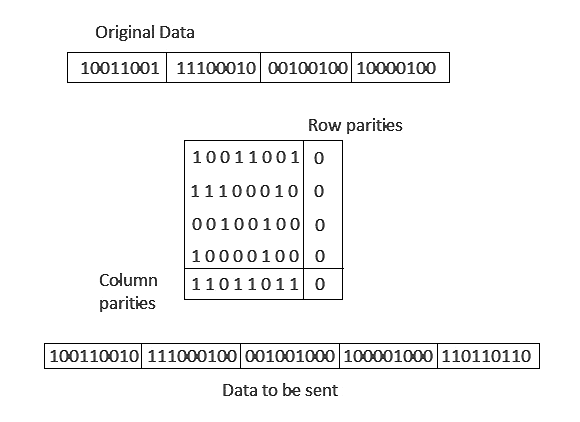
\includegraphics[width=0.75\linewidth]{./images/bidimensionalparitycheck.png}
\end{figure}
\newpage

\subsection{CRC - Cyclic Redundancy Check}
È un metodo di error detection, non correzione. È detto anche controllo dei \textbf{codici polinomiali}. Sfrutta l'aritmetica a $\mod2$, in cui addizione e sottrazione diventano operazioni di $XOR$.

La sequenza di bit $D$ è rappresentata sottoforma di polinomio di grado $d-1=|D|-1$, con coefficienti pari al valore del bit nella sequenza. Il bit più a sinistra è il coefficiente di grado $d-1$ ($x^{d-1}$), quello più a destra è il termine noto ($x^0$). Alla sequenza $D$ \verb|10010111| coinciderà il polinomio:

$$
x^7+ x^4 + x^2 + x^1 + x^0 = x^7+ x^4 + x^2 + x^1 + 1
$$
\begin{itemize}
	\item Sia $D(x)$ il polinomio associato al nostro messaggio $D$.
	\item Sia $G(x)$ il polinomio generatore dello standard di rete. La cifra più significativa è sempre 1.
	\item Sia $r$ il grado di $G(x)$, ed è quindi stabilito dallo standard.
	\item Sia $R(x)=x^r\cdot D(x) \mod G(x)$
\end{itemize}

\subsection{Come effettua il CRC}
Al sender.
\begin{enumerate}
	\item $D$ sono i dati che vogliamo trasmettere.
	\item Calcoliamo $D\cdot 2^r$, nel pratico $D <<r$.
	\item Effettuiamo la divisione $\mod 2$ tra $\frac{D\cdot 2^r}{G}$.
	\item Il resto della nostra divisione sarà il nostro valore di $R$.
	\item Il messaggio che manderemo sarà il risultato della concatenazione di $D+R$. \\In termini di bit: $D\cdot 2^r \ XOR \ \ R$.
	\item Questo valore sarà sempre divisibile per $G$, con resto nullo.
\end{enumerate}

Al receiver.
\begin{enumerate}
	\item Calcola $\frac{\text{Stringa ricevuta}}{G}$.
	\item Se questa divisione ha resto, ci sono stati problemi di trasmissione.
\end{enumerate}

\subsection{Esiti del CRC}
Questo sistema permette di individuare errori a burst al più di $r$ bit. 

\begin{figure}[htp]
	\centering
	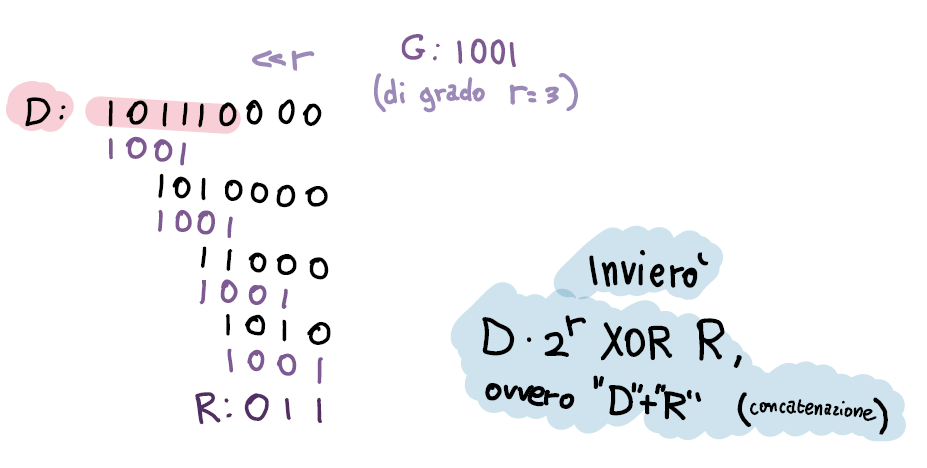
\includegraphics[width=1\linewidth]{./images/crc.png}
\end{figure}

\newpage

\section{Error correction - Perché è difficile?}
Correggere un errore di trasmissione è molto difficile. Il linguaggio naturale gode di contesti (e semantica), tramite cui è possibile estrapolare il significato di una frase, anche quando essa è incompleta!\\ \textit{"Tetto casa rosso" $\to$ "Il tetto della casa è rosso!"}. All'interno di sequenze di bit, non esiste un modo del genere per correggere gli errori. Quello della correzione è un problema molto complesso, verso cui Internet non verte. Quelle di error correction, tuttavia, sono metodologie importanti da conoscere, in quanto utilizzate in molteplici contesti relativi alla trasmissione dati, come all'interno delle RAM.

\subsection{Distanza di Hamming}
Date due codeword, è possibile stabilire una distanza, chiamata \textbf{distanza di Hamming}, che indica il numero di bit che differiscono tra le codeword.
\begin{verbatim}
	10001100 XOR
	11000100  =
	01001000  ->  d=2
\end{verbatim}
Definiamo \textbf{vocabolario} un insieme di codeword. Un vocabolario si dirà \textbf{completo} se, con $n$ bit, avrà $2^n$ codeword.

\subsection{Correzione degli errori - distanza di Hamming}
Limitando un vocabolario a delle stringhe con distanza di Hamming minima fissata, si può ottenere un dizionario del genere:
\begin{figure}[htp]
	\centering
	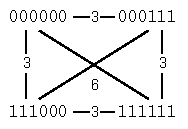
\includegraphics[width=0.5\linewidth]{./images/hamming.pdf}
\end{figure}
con $\min d=3$.\\
Questo limita il numero di stringhe valide, permettendo di introdurre meccanismi di riconoscimento e correzione di errori!
\begin{itemize}
	\item Per \textbf{correggere} $e$ bit di errori, abbiamo bisogno di un vocabolario con distanza minima $d=2e+1$.
	
	
	\item Per \textbf{individuare} $e$ bit di errori, abbiamo bisogno di un vocabolario con distanza minima $d=e+1$.
	
	\begin{figure}[htp]
		\centering
		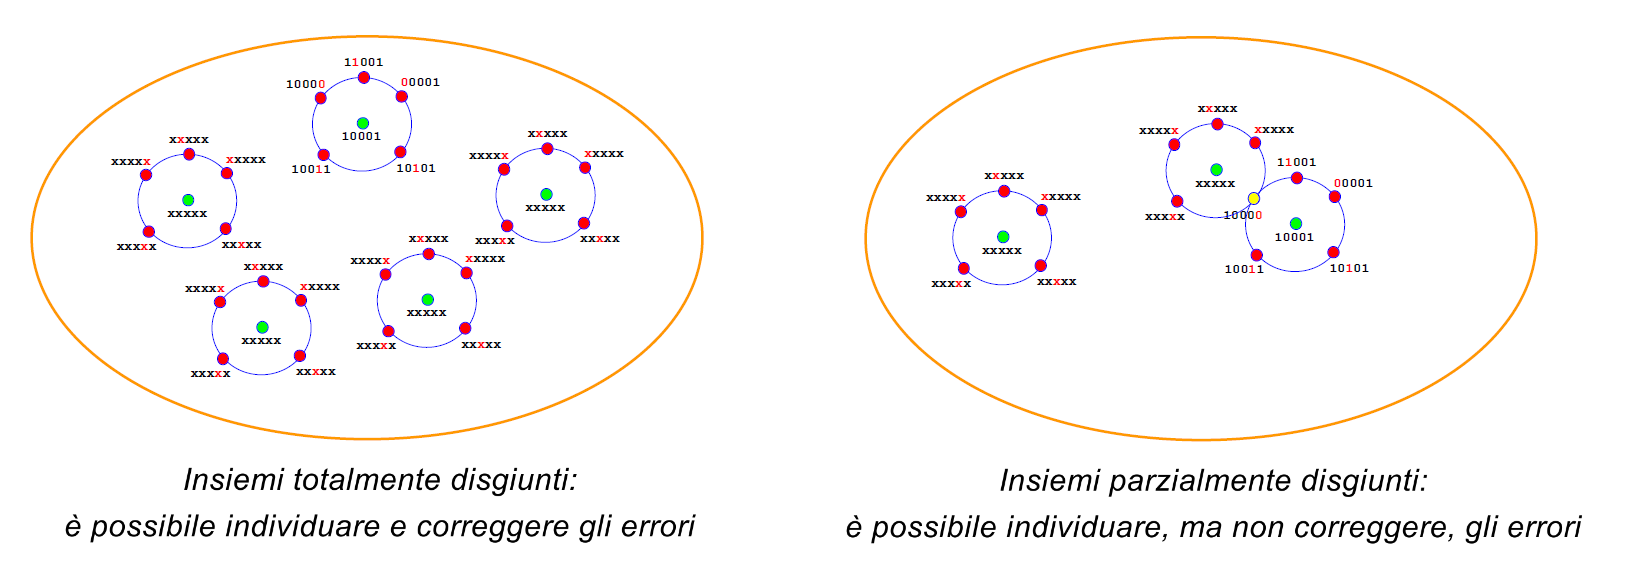
\includegraphics[width=1\linewidth]{./images/correzzioneerrori.png}
	\end{figure}
\end{itemize}

\newpage

\subsection{Dimostrazione distanza minima}
Dato un vocabolario con $m$ bit e $r$ control bit.
$$
m+r = n
$$
Avremo quindi $2^n$ combinazioni, con $2^m$ valide.\\
Data una codeword valida, si ottengono $n$ codeword non valide modificando un singolo bit.

\subsubsection{Formula generale}
$$
\sum _{i=0}^e \binom{m+i}{r} \leq 2^r
$$
Per correggere un errore, avremo:
\begin{footnotesize}
	\begin{verbatim}
		m   r  n  
		1   2  3  
		2   3  5  
		3   3  6  
		4   3  7  
		5   4  9  
		6   4  10 
		7   4  11 
		8   4  12 
		9   4  13 
		10  4  14 
		11  4  15 
		12  5  17 
		
		[...]
	\end{verbatim}
\end{footnotesize}

Per esempio, volessimo trasferire un messaggio di $5$ bit, e volessimo verificare un solo errore $e$, possiamo calcolare:
$$
\sum_{i=0}^{1} \binom{m+i}{r} \leq 2^r
$$
$$
\binom{5}{r} + \binom{6}{r} \leq 2^r
$$
\begin{itemize}
	\item Con $r=0$, $\binom{5}{0} + \binom{6}{0} \leq 2^0 \to 1 + 1 \leq 1 \to 2 \leq 1 $ - falso!
	\item Con $r=1$, $\binom{5}{1} + \binom{6}{1} = \frac{5!}{4!} + \frac{6!}{5!} = \frac{120}{24} + \frac{720}{120} = 5 + 6 = 11 \leq 2^1 $ - falso!
	\item Con $r=2$, $\dots$ - falso
	\item Con $r=3$, $\dots$ - falso
	\item Con $r=4$, $\dots$ - falso
	\item Con $r=5$, $\binom{5}{5} + \binom{6}{5} = 1 + \frac{6!}{5!} = 1 + \frac{720}{120} = 1 + 6 = 7 \leq 2^5 $ - vero!
\end{itemize}

\subsubsection{Reminder utile - formula del coefficiente binomiale}
$$
\binom{n}{k} = \frac{n!}{k!(n-k)!}
$$
\newpage

\subsection{Come si effettua la verifica della distanza di Hamming?}
I bit di controllo sono sempre collocati in posizioni corrispondenti a potenze di due $(1,2,4,8,16,\dots)$.

Il valore del bit di controllo $b_r$ è dato dallo $XOR$ di tutti i valori ottenibili con quel $b_r=1$.\\
Ad esempio, con \verb|xx1x001x0|, abbiamo:
\begin{itemize}
	\item $b_1 = b_3 \ \otimes \ b_5 \ \otimes \ b_7 \ \otimes \ b_9 =  1 \ \otimes \ 0 \ \otimes \ 1 \ \otimes \ 0 = 0$
	\item $b_2 = b_3 \ \otimes \ b_6 \ \otimes \ b_7 = 1 \ \otimes \ 0 \ \otimes \ 1  = 0$
	\item $b_4 = b_5 \ \otimes \ b_6 \ \otimes \ b_7 = 0 \ \otimes \ 0 \ \otimes \ 1  = 1$
	\item $b_8 = b_9 = 0 $
\end{itemize}
E quindi, la stringa che attendiamo, sarà \verb|001100100|.

\subsubsection{Controllo al mittente}
\begin{verbatim}
	001101100
	^^ ^ ! ^
	
	^ = bit da controllare
	| = errore di comunicazione
\end{verbatim}

\begin{itemize}
	\item $b_1 = b_3 \ \otimes \ b_5 \ \otimes \ b_7 \ \otimes \ b_9 =  1 \ \otimes \ 0 \ \otimes \ 1 \ \otimes \ 0 = 0$
	\item $b_2 = b_3 \ \otimes \ b_6 \ \otimes \ b_7 = 1 \ \otimes \ 1 \ \otimes \ 1  = 1$ Errore! Nella stringa ricevuta, $b_2=0$.
	\item $b_4 = b_5 \ \otimes \ b_6 \ \otimes \ b_7 = 0 \ \otimes \ 1 \ \otimes \ 1  = 0$ Errore! Nella stringa ricevuta, $b_3=0$.
	\item $b_8 = b_9 = 0 $
\end{itemize}
L'errore è situato nello slot $b_{2+4} = b_6$. Per correggerlo, effettuiamo un bitflip.
\newpage

\section{Gestire gli accessi multipli}
In una rete, possiamo individuare due tipi di collegamento:
\begin{itemize}
	\item \textbf{Collegamenti punto a punto.}\\
	Sono collegamenti diretti tra trasmittente e ricevente.
	\item \textbf{Collegamenti broadcast.}\\
	Sono collegamenti in cui più nodi trasmittenti e riceventi sfruttano lo stesso canale broadcast.
\end{itemize}

La gestione di un canale broadcast non è un problema per niente intuitivo da risolvere. I protocolli di accesso multiplo gestiscono questo problema, fissando le modalità con cui i nodi regolano le trasmissioni sul canale condiviso.

Quando due nodi cercano di trasmettere sullo stesso canale nello stesso istante, avviene una \textbf{collisione}. Le collisioni causano \textbf{perdite di frame}, e, in eccessiva frequenza, un generale spreco di banda. I \textbf{protocolli di accesso multiplo} gestiscono i canali in maniera consona per non rientrare in situazioni del genere. Esistono tre tipi principali di protocolli per l'accesso multiplo:

\begin{itemize}
	\item \textbf{Protocolli a suddivisione del canale}.\\
	Basati sulla suddivisione del canale in porzioni accessibili esclusivamente ad un nodo.
	\item \textbf{Protocolli ad accesso casuale}.\\
	In cui l'accesso al canale avviene in maniera casuale. Il metodo in questione ammette collisioni, che verranno gestite in maniera opportuna.
	\item \textbf{Protocolli a rotazione - senza collisioni}.\\
	Coordinando opportunamente l’accesso al canale, è possibile evitare le collisioni.
\end{itemize}

\subsection{Protocolli a suddivisione del canale}

\subsubsection{TDMA - Time Division Multiple Access}
Supponiamo una canale broadcast supporti $N$ nodi, e che abbia velocità $R$ bps.\\
TDMA, suddividerà il tempo in \textbf{intervalli di tempo}, e ogni intervallo di tempo in $N$ \textbf{slot temporali}. Ogni slot sarà dedicato ad un nodo: come conseguenza, ogni nodo avrà un tasso di trasmissione di $R/N$ bps. Risolve effettivamente il problema delle collisioni, ma quando si è in uno slot temporale dedicato a un nodo che \textbf{non deve trasmettere nel canale}, avverrà un'attesa non necessaria. 
È un \textbf{protocollo equo}, che \textbf{previene le collisioni}, ma \textbf{limita la banda} di ogni nodo a $R/N$, e porta i nodi in attesa anche quando gli altri non devono trasmettere nulla.

\subsubsection{FDMA - Frequency Division Multiple Access}
Consiste nella suddivisione dello spettro del canale in varie \textbf{bande di frequenza}. A ogni nodo è associata una banda fissa.
Questa suddivisione limita la banda, sempre ad $R/N$, ma non blocca la trasmissione dei nodi.

\subsubsection{CDMA - Code Division Multiple Access}
Consiste nell'associazione di un codice univoco ad ogni nodo. I dati inviati sono codificati secondo quel codice. Con codici opportuni, diventa possibile trasmettere simultaneamente dati a più nodi, e per i nodi, di interpretare in maniera corretta i bit dei dati codificati. Ogni nodo deve conoscere i codici altrui per interpretare correttamente i dati.

\newpage

\subsection{Protocolli ad accesso casuale}
Ogni nodo trasmette alla massima velocità consentita ($R$ bps), e ogni volta che avviene una collisione, i nodi ritrasmetteranno dopo un periodo di tempo casuale (\textit{random delay}). Questo ritardo casuale è indipendente tra i vari nodi, e consente, con buona probabilità, di non subire ulteriori collisioni.\\
\textit{Attenzione, nei seguenti appunti si è deciso di invertire l'ordine con cui, a lezione, sono stati esposti i protocolli ALOHA e Slotted ALOHA. Si è preferito di seguire l'ordine del libro, e di trattare ALOHA come una versione totalmente asincrona di slotted ALOHA}.

\subsubsection{Slotted ALOHA}

\begin{itemize}
	\item Tutti i frame contengono $L$ bit.
	\item Il tempo è suddiviso in slot $L/R$ secondi.
	\item La trasmissione del frame da parte del nodo, inizia all'inizio degli slot.
	\item I nodi sono sincronizzati in modo che tutti sappiano quando iniziano gli slot.
	\item Se in uno slot due o più frame collidono, tutti i nodi della rete rilevano l'evento prima della fine dello slot.
\end{itemize}

Indichiamo $k \in [0,1-K]$, $k, K\in \mathbb{N}$. I nodi slotted ALOHA seguono il seguente comportamento:
\begin{enumerate}
	\item Quando un nodo ha un nuovo frame da spedire, attende l'inizio dello slot successivo, per poi trasmettere il frame.
	
	\item Se non si verifica una collisione, la trasmissione è conclusa.
	
	\item Se si verifica una collisione, il nodo la rileva prima del termine dello slot e ritrasmette il frame dopo $k$ frame, fino a quando l'operazione non ha successo. $k$ è un valore casuale minore di $K$. $K$ cresce ad ogni collisione. 
\end{enumerate}

È un protocollo semplice, che consente ad ogni nodo di lavorare al massimo delle performance possibili, senza limitare i bps a priori. Inoltre, è un protocollo altamente scalabile e abbastanza decentralizzato: l'unica condizione, è che gli slot siano sincronizzati per tutti i nodi.
Tuttavia, ammette collisioni e idle slots, uno spreco generale di slot e un aumento della latenza. 



\subsubsection{Unslotted ALOHA}
È una versione totalmente asincrona dello slotted ALOHA. Il nodo mittente aspetterà un tempo pari al Round Trip Time, in attesa di un ACK. Se l'ACK non arriva, il nodo intuirà che è avvenuta una collisione. In tal caso, aspetterà un quanto di tempo di durata casuale (ma inclusa in un range determinato). Le performance migliori, sono ottenute dalla versione con gli slot temporali.
\begin{figure}[htp]
	\centering
	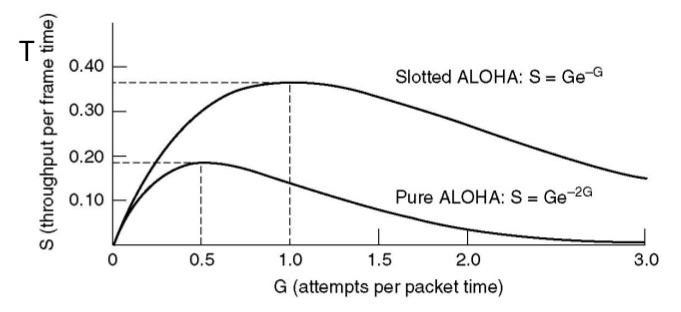
\includegraphics[width=1\linewidth]{./images/ALOHAvsslottedALOHA.png}
\end{figure}

È un grande prezzo da pagare quello per la completa asincronia: l'algoritmo slotted ha un throughput complessivo due volte più grande di quello slotted. L'intuizione è banale: nella versione slotted di ALOHA, due frame possono essere mandati solo all'inizio dello slot temporale. Nella versione unslotted, i frame possono collidere anche a metà trasmissione.

\newpage

\subsubsection{CSMA - Carrier Sense Multiple Access}
I protocolli ALOHA, portano i nodi a decidere di trasmettere indipendentemente dall'attività degli altri nodi. I protocolli CSMA introducono un meccanismo di \textbf{rilevamento della portante} del canale, per "ascoltare" se \textbf{altri nodi stanno già trasmettendo}.
In questo modo, i nodi trasmetteranno esclusivamente quando non rilevano alcuna trasmissione già presente nel canale.\\
Al contrario di ciò che si potrebbe pensare, questo protocollo non sconfigge definitivamente la problematica delle collisioni.
La velocità di trasmissione (nonostante spesso sia altissima) è un fattore non trascurabile.
\begin{enumerate}
	\item Il nodo $A$ trasmette all'istante $t_0$.
	\item $B$ misura la portata del canale all'istante $t_1>t_0$. 
	\item All'istante $t_1$ i bit trasmessi da $A$ potrebbero non essersi propagati fino a $B$.
	\item $B$ trasmette. Collisione!
\end{enumerate}


\subsubsection{CSMA-CD - Carrier Sense Multiple Access con Collision Detection}
Un miglioramento è ottenuto se si introduce un meccanismo di collision detection in aggiunta a quello di rilevamento della portante: la scheda che avrà trasmesso un determinato frame continuerà a misurare il carico del canale. Se rileva rumore o energia di altre trasmissioni nel canale, il nodo interromperà istantaneamente la trasmissione del frame, manderà un \textbf{segnale di jamming con backoff} a tutti gli host, informando tutti i nodi della collisione, e attenderà un quantitativo di tempo casuale per poi ritrasmettere. Questo tempo è chiamato \textbf{tempo di backoff}, non è fissato (intuitivamente renderebbe inutilizzabile il protocollo), e dipende dall'algoritmo scelto dal protocollo.

Un esempio di algoritmo, è quello di \textbf{attesa binaria esponenziale}, o \textit{binary exponential backoff}:
all'$n$-esima collisione, si estrae un valore dall'insieme $K=\{0,1,2,\dots,2^n-1\}$.
Si aspetterà quindi un tempo $T = K \cdot T_\text{slot}$. Il tempo $T_\text{slot}$ dipende dal protocollo: in Ethernet, coincide col tempo richiesto per trasmettere 512 bit, $n$ non supera mai 10, e quindi $0\leq K \leq1023$.

È un ottimo protocollo, ma la collision detection deve avvenire rapidamente: risulta difficile da implementare in reti wireless.

\subsection{Protocolli senza collisioni}
Questi protocolli \textbf{prevengono le collisioni} introducendo dei \textbf{meccanismi preliminari alle trasmissioni}, ottenendo una sincronizzazione consona tra i vari nodi.

\subsubsection{Protocollo bit map - una sorta di prenotazione!}
Con $N$ nodi, il tempo verrà in primis suddiviso in $N$ mini-slot che consentono la trasmissione di un bit. Prima delle trasmissioni effettive, ogni nodo inserirà 1 o 0 nel proprio mini-slot. In questo modo, ogni nodo potrà annunciare se ha intenzione di trasmettere un frame (1) o di non trasmettere (0).
Alla fine di questa trasmissione iniziale, si avrà una \textbf{mappa di bit}, che permetterà ai nodi di seguire un ordine di trasmissione tale da non causare collisioni.

\subsubsection{Binary Backward Counting - una sorta di... torneo?}
In questo protocollo, ogni nodo presenta un ID binario. Questo ID permetterà di risolvere il problema delle collisioni col seguente approccio. Supponiamo $A,B,C,D$ siano dei nodi intenzionati a trasmettere:
\begin{enumerate}
	\item Supponiamo che i nodi $A,B,C,D$ abbiano rispettivamente id \verb|0010|, \verb|1010|, \verb|0100|. \verb|1100|.
	\item Tutti i nodi condividono nel proprio mini-slot, la cifrà più significativa del proprio id.\\
	$A:0$, $B:1$, $C:0$, $D:1$.
	\item Escono dalla competizione i nodi con prima cifra 0. Si passa alla seconda cifra significativa.
	\item $B:0$ $D:1$. $D$ ha vinto la contesa, trasmetterà.
\end{enumerate}

Potrebbe essere unfair sotto determinate circostanze: gli ID binari sono calcolati anche in virtù dei MAC Address, rendendo alcuni dispositivi implicitamente avvantaggiati.

\newpage

\subsubsection{Taking turns protocol}
Ogni nodo manda \verb|1| nel canale per segnalare di voler trasmettere dei frame. I nodi che hanno inviato \verb|1|, si inseriscono in un anello logico. Il primo dei frame di questo nodo sarà il primo a trasmettere. Dopo un tempo $T$, questo nodo passerà un \textbf{token} al prossimo nodo dell'anello, in modo da permettere al prossimo nodo di trasmettere. Tuttavia, \textbf{un guasto di un nodo blocca il sistema} di token-passing. Inoltre, l'anello è un circuito chiuso: occorrerà quindi includere l'intera subnet all'interno dell'anello di trasmissione, per non avere nodi bloccati.

\newpage

\section{Ethernet}
Ethernet è di gran lunga lo standard di reti cablate più diffuso al mondo, per le reti locali. Rappresenta la \textbf{prima LAN ad alta velocità con vasta diffusione}. È riuscito a rimanere al passo tramite versioni via via più veloci, e mantenendo i costi delle componenti hardware non particolarmente alti. È parte dello standard IEEE 802.3.

\subsection{Ethernet CSMA/CD}
È il protocollo d'accesso multiplo al canale condiviso usato da Ethernet. Lo abbiamo trattato nel paragrafo 7.5.2.

\subsection{Tecnologie standardizzate Ethernet}
Le tecnologie standardizzate Ethernet presentano una denominazione fissa:
\begin{itemize}
	\item Un \textbf{numero} che indica la \textbf{velocità dello standard}.
	\item BASE, in quanto trasferisce \textbf{solo traffico Ethernet}.
	\item Un'\textbf{etichetta} che ne specifica il \textbf{mezzo fisico}.
\end{itemize}
\begin{table}[htp]
	\centering
	\begin{tabular}{|c|c|c|c|c|}
		\hline
		Nome & Cavo & Lunghezza massima & Nodi & Vantaggi e caratteristiche note\\
		\hline
		10base5 & Coassiale (spesso) & 500m & 100 & Pirmo cavo: ormai deprecato\\
		\hline
		10base2 & Coassiale (snello)& 185m & 30 & Non richiede un hub\\
		\hline
		10base-T & UTP & 100m & 1024 & Sistema più economico\\
		\hline
		10base-F & Fibra Ottica & 2000m & 1024 & Copre grandi distanze\\
		\hline
	\end{tabular}
	\caption{Tecnologie Ethernet a 10Mbps}
\end{table}

Il coassiale spesso soffre per la sua estrema rigidità, il coassiale snello si rompe troppo facilmente.

\begin{table}[htp]
	\centering
	\begin{tabular}{|c|c|c|c|c|}
		\hline
		Nome & Cavo & Lunghezza massima & Nodi & Vantaggi e caratteristiche note\\
		\hline
		100base-T4 & UTP & 100m &  & Economico, encoding 8B6T\\
		\hline
		100base-TX & UTP & 100m &  & Full Duplex, encoding 4B5B\\
		\hline
		100base-FX & Fibra Ottica & 2000m &  & Copre grandi distanze\\
		\hline
	\end{tabular}
	\caption{Tecnologie Ethernet a 100Mbps}
\end{table}

Un'estensione degli standard Ethernet è Gigabit Ethernet, detto anche IEE 802.3z.
\begin{table}[htp]
	\centering
	\begin{tabular}{|c|c|c|c|c|}
		\hline
		Nome & Cavo & Lunghezza massima & Nodi & Vantaggi e caratteristiche note\\
		\hline
		1000Base-SX & Fibra multimodale & 550m &  & Più segnali simultanei\\
		\hline
		1000Base-LX & Fibra multimodale & 5000m &  &  Copre grandissime distanze\\
		\hline
		1000Base-CX & 2 coppie di STP & 25m &  & \\
		\hline
		1000Base-T & 4 coppie di UTP  & 100m &  & Full Duplex, encoding a 5 livelli\\
		\hline
	\end{tabular}
	\caption{Tecnologie Ethernet a 1Gbps}
\end{table}

Inoltre, 1000Base-T non usa il 4B5B e introduce un \textbf{forward error correction}.
\newpage

\subsection{Cavi}
La trasmissione di un cavo è influenzata dal come è stato realizzato. Alcuni fattori da tenere in considerazione, sono i seguenti:

\begin{itemize}
	\item Il passaggio di corrente, che induce un \textbf{campo magnetico}, crea \textbf{corrente indotta}. Questa scorre dal verso opposto al flusso di corrente di partenza, il quale subirà una vera e propria \textbf{opposizione}. Anche i cavi adiacenti posso creare campi magnetici e quindi flussi opposti: questo fenomeno si chiama \textbf{diafonia}.
	
	\item La \textbf{lunghezza} del cavo è \textbf{direttamente proporzionale} alla sua \textbf{resistenza}: per coprire grandi distanze, è necessario usare dei \textbf{ripetitori}.
\end{itemize}

\subsubsection{Parti dei cavi di rame}
\begin{itemize}
	\item \textbf{Conduttore}.
	\item \textbf{Jacket}.\\
	Materiale isolante esterno.
	\item \textbf{Shield}.\\
	Schermatura complessiva su tutti i cavi.
	\item \textbf{Foil}.\\
	Schermatura su una coppia di cavi.
\end{itemize}
Detto ciò, \textbf{UTP} sta per \textbf{Unshielded Twisted Pair}, \textbf{STP} sta per \textbf{Shielded Twisted Pair}, \textbf{FTP} sta per \textbf{Foiled Twisted Pair}, \textbf{SFTP} sta per \textbf{Shielded Foiled Twisted Pair}.

\subsubsection{Categorie cavi di rame}
\begin{itemize}
	\item \textbf{Cat5}, che supporta fino a 100Mbps e opera sui 100Mhz di frequenza;
	\item \textbf{Cat5e} (Cat5 enhanced), che segue maggiormente gli standard IEE e supporta fino a 1Gbps, operando sempre su 100Mhz di frequenza;
	\item \textbf{Cat6}, che supporta fino a 10Gbps e opera sui 250Mhz di frequenza;
	\item \textbf{Cat6a}, che supporta fino a 10Gbps, ma con maggiori distanze e sulla frequenza di 500Mhz.
\end{itemize}

\newpage

\subsection{Connettore RJ-45}
È la terminazione dei cavi usati da Ethernet. Sono del tipo 8P8C (otto posizioni, otto contatti). Esistono inoltre due schemi di cablaggio, T568A e T568B, che differiscono per un'inversione delle coppie 2 e 3. T568B è il prediletto nei sistemi recenti, secondo lo standard ANSI/TIA ((American National Standards Institute e Telecommunications Industry Association).


\begin{figure}[htp]
	\centering
	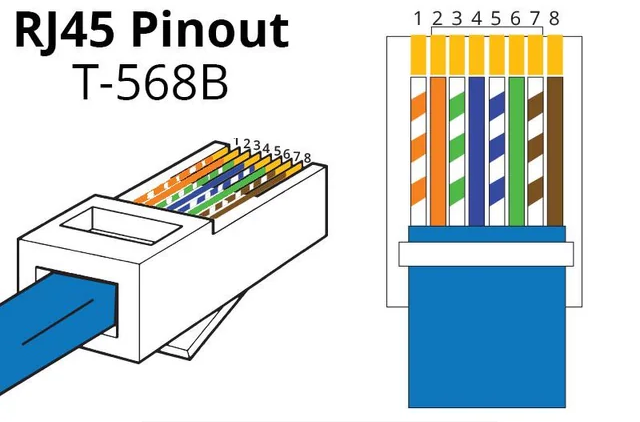
\includegraphics[width=0.4\linewidth]{./images/RJ45.png}
\end{figure}

\begin{table}[htp]
	\centering
	\begin{tabular}{|c|c|c|c|}
		\hline
		Pin & Colore & Polarità & Utilizzo\\
		\hline
		1 & bianco/arancione & + & Trasmissione (Tx)\\
		2 & arancione & - & Trasmissione (Tx)\\
		3 & bianco/verde & + & Ricezione dati (Rx)\\
		4 & blu & - & Bidirezionale dati (Bi3)\\
		5 & bianco/blu & + & Bidirezionale dati (Bi3)\\
		6 & verde & - & Ricezione dati (Rx)\\
		7 & bianco/marrone & + & Bidirezionale dati (Bi4)\\
		8 & marrone & - & Bidirezionale dati (Bi4)\\
		\hline
	\end{tabular}
\end{table}

La polarità opposta nei segnali trasmessi nei cavi twisted pair permette di ridurre il rumore con estrema facilità.
Supponiamo che un bit venga trasmesso a 1V in due coppie di cavi con polarità opposta ($A: +1V$,  $B: -1V$). Nei sistemi \textbf{differenziali}, il segnale sta nella differenza tra le coppie di segnali, e quindi:
$$
1 V - (-1V) = 1V+1V = 2V
$$

Supponiamo adesso di indurre un rumore di $+0.5V$ al nostro cavo (e quindi su entrambi i cavi della coppia). 

$$
(1V+0.5V) - (0.5V-1V) = 1.5V - (-0.5V)=1.5V+0.5V = 2V
$$

\begin{figure}[htp]
	\centering
	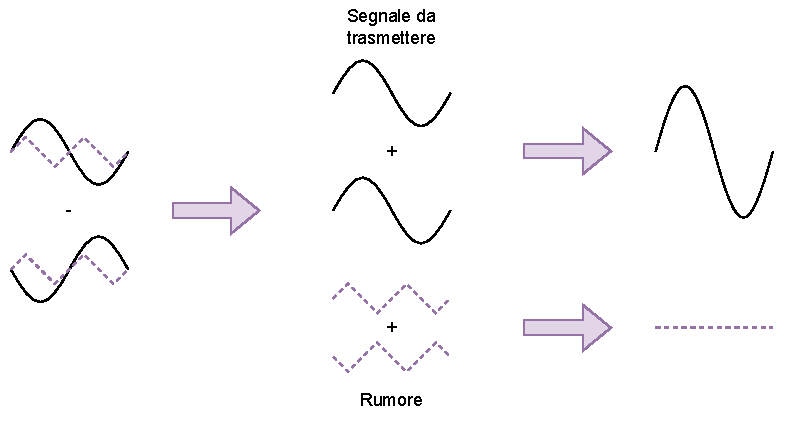
\includegraphics[width=0.85\linewidth]{./images/noise canceling (1).pdf}
	\caption{Esempio di cancellazione del rumore}
\end{figure}

\newpage

\subsubsection{Distinzione: cavi diretti e cavi incrociati}
\begin{itemize}
	\item \textbf{Cavo incrociato.}\\
	La disposizione dei doppini è diversa tra le due estremità. È usato per collegare dispositivi simili (router a router).
	\item \textbf{Cavo diretto.}\\
	La disposizione dei doppini è uguale tra le due estremità. È usato per collegare dispositivi diversi (pc a router).
\end{itemize}
\section{Frame Ethernet}
\begin{figure}[htp]
	\centering
	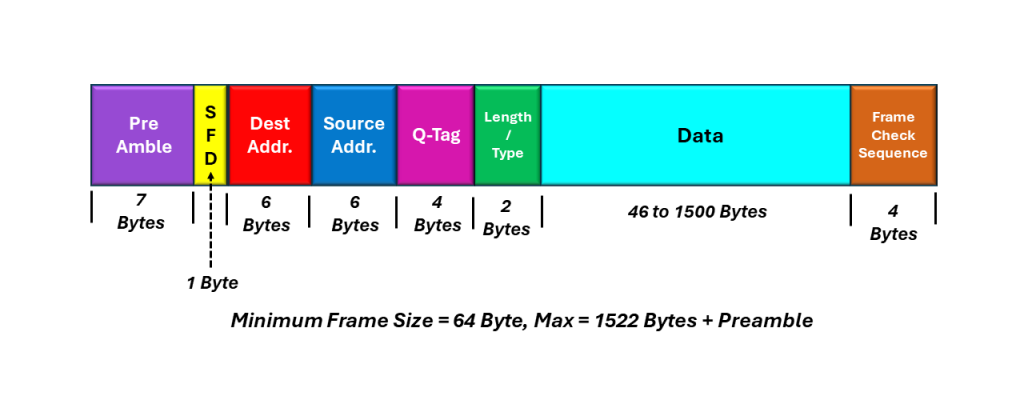
\includegraphics[width=1\linewidth]{./images/frameethernet.png}
\end{figure}
\begin{itemize}
	\item \textbf{Preambolo}.\\
	7 byte a \verb|10101010| per sincronizzare i clock delle schede di rete.
	\item \textbf{Start Frame Delimiter}.\\
	Un byte a \verb|10101011| per interrompere il pattern del preambolo e indicare l'inizio del frame.
	\item \textbf{MAC address destinatario}.\\
	6 byte.
	\item \textbf{MAC address mittente}.\\
	6 byte.
	\item \textbf{Q-Tag/VLAN Tag}.\\
	È il tag presente \textbf{esclusivamente nei frame Ethernet che supportano le VLAN}. Non è sempre presente, in quanto non tutti i frame Ethernet sono \textit{tagged}. 4 byte.
	\item \textbf{Type/length}.\\
	2 byte che identificano il tipo di connessione (EtherType, IPv4, IPv6, ARP,$\dots$), se ha valore superiore a 1500, altrimenti, la lunghezza del data field.
	\item \textbf{Data field}.\\
	Minimo 46 byte, massimo 1500 byte. Se il frame da inviare non supera la dimensione minima, si usa un \textbf{padding}. Se il frame supera la dimensione massima, si frammenta.
	\item \textbf{Frame check sequence}.\\
	4 byte dedicati al controllo CRC per rilevare (e/o correggere) errori.
\end{itemize}

\newpage

\subsection{Codifica di Manchester}
È una codifica che nasce per ovviare ad alcune delle criticità relative alla trasmissione che già conosciamo:
\begin{itemize}
	\item \textbf{Ambiguità delle lunghe sequenze.}\\
	La codifica di Manchester forza delle transizioni obbligatorie quando trasmette dei bit. Diventa più facile riconoscere malfunzionamenti e interruzioni della trasmissione.
	\item \textbf{Sincronizzazione precaria.}\\
	Ogni bit contiene al suo interno una transizione. Non può perdersi la sincronizzazione.
\end{itemize}

Viene realizzata tramite un'operazione di $XOR$ tra il segnale di clock e il segnale dati. Ogni bit è codificato come un fronte di salita (1) o un fronte di discesa (0). In questo modo, il \textit{bitstream} e il segnale di clock sono, in un certo senso, trasmessi contemporaneamente.

\begin{figure}[htp]
	\centering
	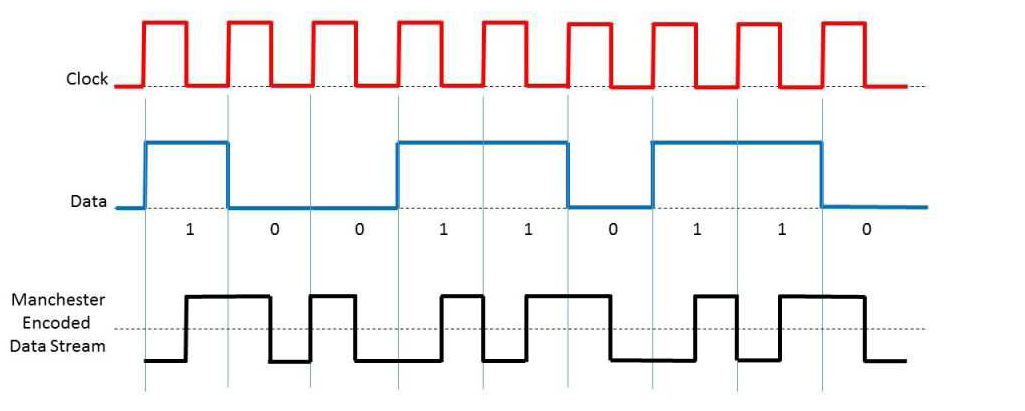
\includegraphics[width=1\linewidth]{./images/manchesterencoding1.png}
\end{figure}

Tuttavia, questa codifica è influenzata dalla polarità del segnale trasmesso. Se il segnale codificato viene invertito, bisogna invertire anche la sua codifica. Possiamo risolvere il problema usando la codifica di Manchester differenziale.


\subsubsection{Codifica di Manchester differenziale}
Rende la codifica di Manchester insensibile alla polarità. Ogni bit presenta almeno una transizione a metà periodo di clock. Il valore del bit dipenderà dalla presenza o meno di una transizione (in particolare, fronte di salita) all'inizio del periodo di clock.
\begin{itemize}
	\item Bit 0: transizione.
	\item Bit 1: assenza di transizione.
\end{itemize}

\begin{figure}[htp]
	\centering
	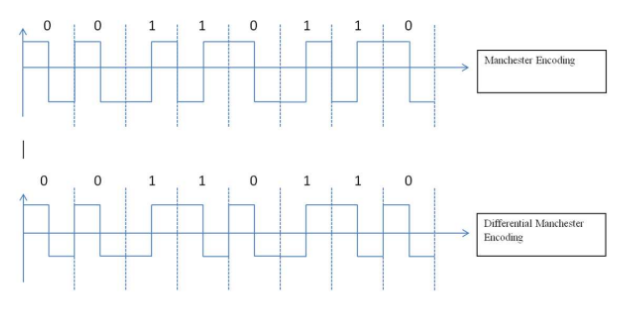
\includegraphics[width=0.8\linewidth]{./images/Manchester.png}
	\caption{Codifiche di Manchester a confronto}
\end{figure}

\newpage

\section{Gigabit Ethernet}
È lo standard Ethernet che raggiunge i 1000Mbps, ovvero 1Gbps. Andiamo a scomporre come le scelte prese permettano di raggiungere queste velocità.
\begin{enumerate}
	\item \textbf{Rimossa la codifica 4B5B.}\\
	$100 \to 125$ Mbps. Rimuoviamo l'overhead del $25\%$ della codifica 4B5B. La sincronizzazione è garantita dalla codifica di Manchester.
	
	\item \textbf{4 doppini di rame usati allo stesso tempo}.\\
	$125 \to 4\cdot125 = 500$ Mbps.
	
	\item \textbf{Trasmissione full-duplex}.\\
	$500$ Mbps full-duplex.
	
	\item \textbf{5 livelli per baud invece di 3}.\\
	5 livelli su ogni canale di trasmissione. Con 4 canali, otteniamo $5^4=625$ combinazioni, e quindi $\log_2(625) \approx 9$ bit
	
	\item \textbf{Trasmissione finale:} Con $10^6$ frequenza di simbolo $125 \cdot 10^6 \cdot 9$bit = 1 Gbit lordo.
	
	\item \textbf{Forward Error Correction}.
\end{enumerate}

\subsection{Filtro DuoBinary}
Il seguente filtro, detto DuoBinary, si occupa della codifica.
\begin{figure}[htp]
	\centering
	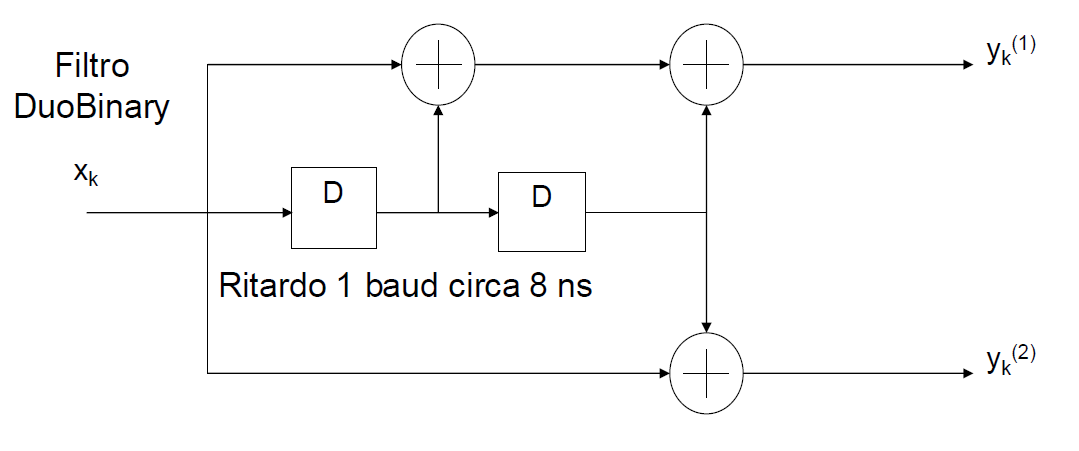
\includegraphics[width=0.75\linewidth]{./images/duobinary.png}
\end{figure}

\begin{enumerate}
	\item Il bit in entrata viene sdoppiato in due segnali.
	\item Introduce un ritardo ad uno dei due segnali.
	\item Si stringe lo spettro del segnale: \textbf{un simbolo viene codificato in due simboli}.
\end{enumerate}

\newpage

\subsection{Decodifica 4D}
La decodifica 4D, detta di Viterbi, viene eseguita tramite un automa a stati finiti.

\begin{figure}[htp]
	\centering
	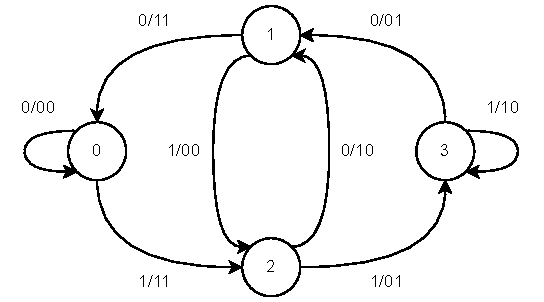
\includegraphics[width=0.75\linewidth]{./images/trellis.drawio.pdf}
\end{figure}

Ciò che viene fatto è una \textbf{Trellis code modulation}. Raddoppiando il numero di bit per rappresentare un bit d'informazione, gli errori peseranno meno sull'informazione complessiva. Tuttavia è grazie alle transizioni dell'automa limitate che è possibile capire quando è avvenuto un errore: la distanza di Hamming delle stringhe possibili valutate rispetto a quella consegnata, ci permette di stabilire come effettuare la correzione.

\newpage

\section{Strutture Ethernet}
Hub e bridge sono strutture fisiche che permettono di collegare le varie sottoreti. Sono strutture molto diverse, e al giorno d'oggi l'hub è obsoleto. Il bridge è alla base di tutti gli switch moderni.

\subsection{Differenze tra hub e bridge}
L'ormai obsoleto hub:
\begin{itemize}
	\item Lavora principalmente al livello fisico.
	\item Ripete e rigenera il segnale su tutte le porte.
	\item Il dominio di collisione tra tutti i dispositivi collegati è unico.
	\item Broadcast domain unico. 
\end{itemize}
Il bridge, invece:
\begin{itemize}
	\item Lavora a livello data link.
	\item Filtra e inoltra in base all'indirizzo MAC 
	\item Nel bridge ogni porta crea (idealmente) un dominio di collisione separato.
	\item Broadcast domain unico.
\end{itemize}

\subsection{Switch}
È un dispositivo che trasmette pacchetti ricevuti a uno o più dispositivi destinatari. È più espandibile in termini di numero di porte, rispetto al bridge, ed effettua operazioni di \textbf{inoltro} (individuare a quale interfaccia mandare il frame) e \textbf{filtraggio} (capire quando scartare un frame). Uno switch contiene al suo interno una \textbf{switch table} con record del tipo \verb|Indirizzo MAC - Interfaccia - Tempo|.
Il tempo viene utilizzato per stabilire quando un dispositivo non è più presente nella rete: verrà dedotto in quanto non verranno mandati più pacchetti al suo indirizzo MAC per molto tempo. Gli switch sono full duplex, senza collisioni.

\newpage


\section{VLAN}
Le LAN virtuali permettono di creare delle LAN logiche indipendenti sulla stessa struttura fisica. 

\begin{figure}[htp]
	\centering
	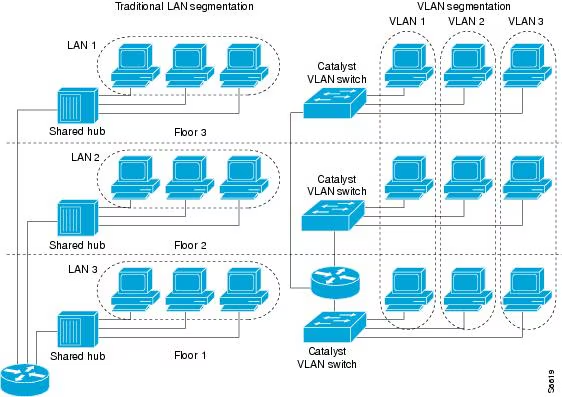
\includegraphics[width=0.75\linewidth]{./images/vlan.png}
\end{figure}

Permette di risparmiare su costi, sulla manodopera e sulla complessità dietro il ricablaggio di una rete, per modificarne la struttura logica. Sono quindi delle vere e proprie LAN logiche separate che risiedono sopra la struttura fisica. Le LAN virtuali rimappano le tabelle di forward del bridge senza modificare la cablatura. Una porta può essere associata a una e una sola VLAN, altrimenti si riscontrerebbero collisioni.

\subsection{Scopo delle VLAN}
\begin{itemize}
	\item \textbf{Riutilizzo dell'architettura di partenza} con conseguente risparmio.
	\item \textbf{Flessibilità}.\\
	Molto più facile spostare gli utenti tra le VLAN.
	\item \textbf{Prestazioni migliori}.\\
	Isolando il broadcasting nelle VLAN,
	\item \textbf{Sicurezza}.\\
	È semplice isolare dei sistemi tramite le VLAN.
\end{itemize}

\subsection{VLAN basata su porte}
Lo switch può essere \textbf{partizionato logicamente} in più insiemi di porte. Le porte possono essere associate a delle VLAN. Nell'header dei frame DLL è presente un identificatore di VLAN.

\begin{itemize}
	\item \textbf{Tag Protocol Identifier.}\\
	16 bit.
	\item \textbf{Priority.}\\
	Identifica il livello di priorità. 3 bit.
	\item \textbf{Canonical Format Identifier.}\\
	1 bit che specifica se il frame è untagged. Il flag a 0 indica che il meccanismo di VLAN non è supportato.
	\item \textbf{Virtual Lan Identifier.}\\
	12 bit.
\end{itemize}



\newpage

\subsection{LAN vs Dispositivi Legacy}
I dispositivi legacy che non supportano le VLAN, ignorano tutti i frame tagged VLAN a loro in arrivo.

\begin{figure}[htp]
	\centering
	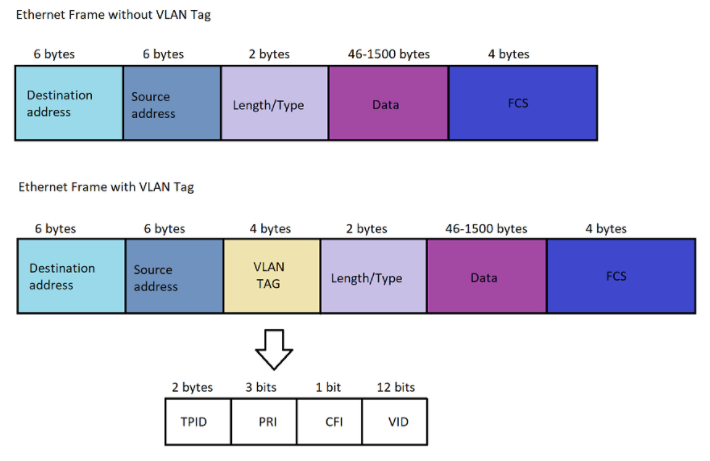
\includegraphics[width=0.75\linewidth]{./images/vlanvslegacy.png}
\end{figure}

\begin{figure}[htp]
	\centering
	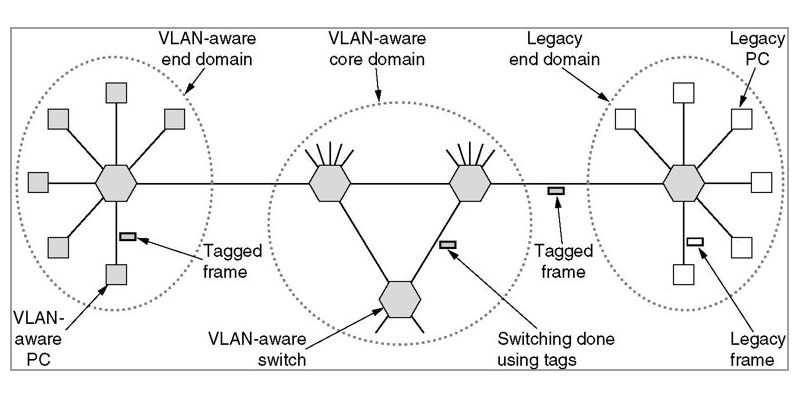
\includegraphics[width=1\linewidth]{./images/VLAN3.png}
	\caption{Una rete con dispositivi VLAN e legacy}
\end{figure}


\chapter{Esercizi}

\section{Polinomi}
Calcola il resto $R(x)$ della seguente divisione polinomiale in $\mathbb{Z}^2$. 

$$
\frac{(x^5 + x + 1) (x^4 + x^2 + 1) + (x^2+1)}{(x^2 + x)}
$$

Facilitiamo l'esercizio suddividendolo in singoli polinomi.
\begin{itemize}
	\item $A(x) = (x^5 + x^1 + 1)$;
	\item $B(x) = (x^4 + x^2 + 1)$;
	\item $C(x) = (x^2 + 1)$;
	\item $D(x) = (x^2 + x)$;
\end{itemize}

Svolgiamo le operazioni.
\begin{enumerate}
	\item $A(x) \cdot B(x) = (x^9 + \cancel{x^5} + x^4 + x^7 + x^3 + x^2 + \cancel{x^5} + x + 1)$
	
	\item $A(x) \cdot B(x) + C(x) = (x^9 + x^4 + x^7 + x^3 + \cancel{x^2} + x + \cancel{1}) +  (\cancel{x^2} +\cancel{1}) = (x^9 + x^7+ x^4 + x^3 + x)$. 
	
	Abbiamo letteralmente effettuato uno $XOR$. Chiameremo $E(x)$ il polinomio risultante.
	
	\item $E(x)/D(x)$. Facciamo delle osservazioni.
	\begin{itemize}
		\item $E(x) = \verb|1010011010|$
		\item $D(x) = \verb|110|$
	\end{itemize}
	
	Facciamo la divisione.
	
	\begin{verbatim}
		1010011010  |
		110         |
		-------------
		11         |
		110        |
		-------------
		110    |
		110    |
		------------
		10  | resto trovato
	\end{verbatim}
	
	$R(x) = \verb|10| = 1\cdot x^1 + 0\cdot x^0 = x$;
\end{enumerate}

Soluzione: $R(x) = x$.









\end{document}